\documentclass[a4paper, 12pt]{article}

\usepackage{cmap}
\usepackage[T2A]{fontenc}
\usepackage[english, russian]{babel}
\usepackage[utf8]{inputenc}
\usepackage[left=2cm,right=1.5cm,top=2cm,bottom=2cm]{geometry}
% \usepackage{mathtext}
\usepackage{amsmath}
\usepackage{amssymb}
\usepackage{etoolbox}
\usepackage{amsthm}
\usepackage{booktabs}
% \usepackage{nicematrix}
\usepackage{graphicx}
% \usepackage{tikz}
% \usepackage{parskip}

%Реализация aug, overbrace и underbrace без nice matrix
\newcommand\aug{\fboxsep=-\fboxrule\!\!\!\fbox{\strut}\!\!\!}
\newcommand\undermat[2]{\makebox[0pt][l]{$\smash{\underbrace
{\phantom{\begin{matrix}#2\end{matrix}}}_{\text{$#1$}}}$}#2}
\newcommand\overmat[2]{\makebox[0pt][l]{$\smash{\overbrace
{\phantom{\begin{matrix}#2\end{matrix}}}^{\text{$#1$}}}$}#2}
\newcommand\tab[1][.5cm]{\hspace*{#1}}
\newcommand\Underset[2]{\underset{\textstyle #1}{#2}}
\newcommand\Overset[2]{\overset{\textstyle #1}{#2}}


\theoremstyle{definition}
\newtheorem*{definition}{Определение}
\newtheorem*{theorem}{Теорема}
\newtheorem*{consequense}{Следствие}
\newtheorem*{lemma}{Лемма}
\newtheorem*{subtheorem}{Утверждение}
\newtheorem*{remark}{Замечание}


\begin{document}
    \fontsize{14pt}{20pt}\selectfont
    \begin{center}
        \begin{LARGE}
            \textbf{Линейная алгебра и геометрия}
        \end{LARGE}

        \begin{Large}
            \textbf{Глава I. Векторное пространство}
            % \newline
            
            \textbf{\S1. Векторное пространство, размерность, изоморфизм}
        \end{Large}
    \end{center}

    \begin{definition}
        Множество $V$ называется
        \textit{векторным пространством}
        над полем $F$, если заданы операции $+$ и $\cdot$\ :
        $V\times V \to V$, $F \times V \to V$ 
        и выполнены следующие аксиомы: 

        1. $\forall v_1, v_2, v_3\in V$ выполнено
        $(v_1 + v_2) + v_3 = v_1 + (v_2 + v_3)$

        2. $\exists \vec 0 \in V:\ \forall v \in V$
        выполнено $v + \vec 0 = v$

        3. $\forall v \in V \ \ \exists  -v  \in V$:
        $v + (-v) = \vec 0$

        4. $\forall v_1, v_2 \in V$ выполнено 
        $v_1 + v_2 = v_2 + v_1$

        5. $\forall \alpha, \beta \in F, v \in V$ 
        выполнено $(\alpha \beta)v = \alpha (\beta v)$

        6. $\forall v \in V$ выполнено $1 \cdot v = v$

        7. $\forall \alpha, \beta \in F, v \in V$ выполнено
        $(\alpha + \beta)v = \alpha v + \beta v$

        8. $\forall \alpha \in F, v_1, v_2 \in V$ выполнено
        $\alpha (v_1 + v_2) = \alpha v_1 + \alpha v_2$        
    \end{definition}

    \begin{subtheorem}
        Линейным операциям над векторами соотвествует такие же
        операции над их координатами: 
        
        1. $x = eX, y = eY \Rightarrow x + y = e(X + Y)$

        2. $\lambda x = e(\lambda X)$
    \end{subtheorem}
    \begin{proof}
        Пусть $e = (e_1, e_2,...,e_n)$ базис в $V$.
        Тогда $$x = \sum\limits_{i=1}^n x_i e_i =
        (e_1, e_2,..., e_n)
        \begin{pmatrix}
            x_1\\
            x_2\\
            \vdots\\
            x_n
        \end{pmatrix}
        = eX$$
    \end{proof}
    \begin{definition}
        $\varphi: V \to W$ \textit{линейно}, если:

        1. $\forall v_1, v_2 \in V$ выполнено
        $\varphi (v_1 + v_2) = \varphi (v_1) + \varphi (v_2)$

        2. $\forall v \in V, \lambda \in F$ выполнено
        $\varphi (\lambda v) = \lambda \varphi (v)$
    \end{definition}
    \begin{definition}
        $\varphi$ называется \textit{изоморфизмом}, если
        $\varphi$ линейно и биективно.
    \end{definition}
    \begin{consequense}
        Если $\varphi$ линейное отображение, то $\varphi
        (\vec 0_V) = \varphi (\vec 0_W)$
    \end{consequense}
    \begin{proof}
        $$\vec 0_V + \vec 0_V = \vec 0_V \Rightarrow 
        \varphi (\vec 0_V + \vec 0_V) = \varphi (\vec 0_V) +
        (-\varphi (\vec 0_V)) \Rightarrow 
        \varphi(\vec 0_V) = \vec 0_W \Leftrightarrow
        dimV = dimW$$
    \end{proof}
    \begin{consequense}
        $dimV=n \Leftrightarrow V \cong F^n$, где $F^n$
        пространство столбцов высоты n.
        
        ("$\cong$" Чубаров обозначает изоморфность)
    \end{consequense}
    \begin{proof}
        $\Longleftarrow $ Пусть $V \cong W$
        изоморфизм $\Rightarrow dimV=dimW$.
        По условию $\exists \varphi: V \to W$
        изоморфизм. Фиксируем базис $(e_1, e_2,..., e_n)$ в $V$ и
        покажем, что \\$\varphi (e_1), \varphi (e_2),...,
        \varphi (e_n)$ базис в $W$.\\
        1. $\varphi (e_1), \varphi (e_2),...,\varphi (e_n)$
        - ЛНЗ и $\sum \limits_{i=1}^{n} \lambda_i \varphi (e_i)
        = \vec 0_W \Rightarrow \sum \limits_{i=1}^{n} \varphi 
        (\lambda_i e_i) = \vec 0_W,$

        $\varphi$ - инъективно, но $\varphi (\vec 0_V) = \vec 0_W
        \Rightarrow \sum \limits_{i=1}^{n} \lambda_i
        e_i = \vec 0_V \Rightarrow$ все $\lambda_i = 0$\\
        2. $\varphi (e_1), \varphi (e_2),..., \varphi (e_n)$
        - полная система: $\forall w \in W\  \exists v \in V:
        \varphi (v) = w$, так как $\varphi$ - сюръективна.
        $\Rightarrow \exists x_1, x_2,..., x_n \in F$;
        $v = \sum \limits_{i=1}^n x_ie_i \Rightarrow 
        \varphi (v) = w = \sum\limits_{i=1}^n x_i\varphi (e_i)
        \Rightarrow \varphi(e_1), \varphi(e_2),...,
        \varphi(e_n)$ - базис в W.

        $\Longrightarrow $ Пусть $dimV = dimW = n.$ Построим
        изоморфизм. Фиксируем базис $e = (e_1, e_2,...,e_n)$
        в $V$ и $f = (f_1, f_2,...,f_n)$ в $W$. Положим:
        $\varphi (e_i) = f_i$. Достроим $\varphi$ до
        линейного отображения, так что $\forall v \in V$
        выполнено $v = \sum\limits_{i=1}^n x_ie_i$.
        Тогда $\varphi (v) = \varphi (\sum\limits_{i=1}^n x_ie_i)
        = \sum\limits_{i=1}^n x_i \varphi (e_i) =
        \sum\limits_{i=1}^n x_if_i$. Таким образом, $\varphi$
        линейно.

    \end{proof}
    \underline{\textbf{Замена базиса}}

    Пусть $dimV = n, e = (e_1,...,e_n)$ - старый базис,
    $e' = (e_1',...,e_n')$ - новый базис.
    
    Пусть известно, что $\forall e_j'$ выполнено $$e_j' = 
    \sum\limits_{i=1}^n c_{ij}e_i = e
    \begin{pmatrix}
        c_{1j}\\
        \vdots\\
        c_{nj}
    \end{pmatrix}
    \Leftrightarrow e'= eC_{e \to e'},$$
    
    где $ C=(c_{ij})$.
    \begin{lemma}
        1. $det\ C\neq 0$

        \ \ \ \ \ \ \ \ \ 2. $C_{e'\to e}=C_{e\to e'}^{-1}$
    \end{lemma}
    \begin{theorem}
        Пусть $e, e'$ два базиса в пространстве $V$,
        $X_e$ и $X_{e'}$ столбцы координат одного и тоже вектора.
        Тогда $X_e = CX_{e'}$
    \end{theorem}
    \begin{proof}
        $\forall x\in V$ выполнено $$x= eX_e= e'X_{e'}= 
        eC_{e\to e'}X_{e'}= e(C_{e\to e'}X_{e'})$$
    \end{proof}
    \newpage
    \begin{center}
        \begin{Large}
            \textbf{\S2. Подпространство}
        \end{Large}
    \end{center}
    \begin{definition}
        Подмножество $U$ в пространстве $V$ называется\\
        \textit{подпространством} в $V$, если:

        1. $\forall U\neq 0$

        2. $\forall u_1, u_2 \in U$ выполнено $u_1 + u_2 \in U$

        3. $\forall u \in U, \lambda \in F$ выполнено
        $\lambda u\in U$
    \end{definition}
    \textbf{Способы задания подпространства:}

    1. $U =\langle a_1, a_2,..., a_n\rangle$

    $2.\ dimV = n,\ W = \{v = eX|AX = 0\}$

    \begin{definition}
        \textit{Линейная оболочка векторов} $a_1, a_2,...,a_n
        \in V$ -- это\\ $\tab[3.6cm]\{\lambda_1a_1 + \lambda_2a_2 + ... + 
        \lambda_na_n|\lambda_i \in F\}$
    \end{definition}
    \begin{lemma}
        1. $\langle a_1, a_2,..., a_m \rangle := U$ -- подпространство в $V$

        $\tab[1.4cm]2. dim\ U = rk\{a_1, a_2,..., a_m\}$
    \end{lemma}
    \begin{proof}
        Если $dim\ U = n$, то фиксируем базис и составляем
        матрицу из столбцов координат $a_1, a_2,..., a_m:$
        $$A = (a_1^\uparrow, a_2^\uparrow,...,a_m^\uparrow)\sim
        \begin{pmatrix}
            a_{1j_1} & \hdotsfor{7}\\
            0 & a_{1j_2} & \hdotsfor{6}\\
            \hdotsfor{8}\\
            0 & 0 & \dots & \hdotsfor{3} & a_{rj_r} & \dots\\
            \hdotsfor{8}\\
            0 & 0 & \hdotsfor{6}
        \end{pmatrix}$$
        Элементарными преобразованиями строк приводим матрицу A
        к ступенчатому виду и получаем, что столбцы $a_{j_1},
        a_{j_2},..., a_{j_r}$ составляют бызис в $U$.\\
    \end{proof}
    \begin{lemma}
        Любую ЛНЗ систему векторов в $V (dimV < \infty)$ можно
        можно дополнить до базиса пространства $V$.
    \end{lemma}
    \underline{\textbf{Алгоритм}}: Пусть $a_1, a_2,..., a_m$ - ЛНЗ,
    $m < n = dimV$, известны координаты этих векторов в
    некотором базисе. Тогда $rk(a_1^\uparrow, a_2^\uparrow,...,
    a_m^\uparrow) = m.$ Составим матрицу столбцов из них и
    припишем столбцы $E$ порядка n:
    $$(A|E_n) \sim 
    \begin{pmatrix}
        \text{Выделим базисные столбцы}\\
        \text{Э.П. строк в \(A|E_n\),}\\
        \text{включая столбцы A}
    \end{pmatrix}
    \sim rk(A|E_n) = n$$\\
    Вывод: к $a_1, a_2,..., a_m$ надо добавить единичные столбцы,
    вошедшие в базис матрицы $A|E_n$.
    \newpage
    \begin{center}
        \underline{\textbf{Операции с блочными матрицами}}
    \end{center}
    \begin{definition}
        \textit{Блочная матрица} -- матрица, разбитая на
        подматрицы, которые обозначаются отдельными буквами.
    \end{definition}
    \textbf{Пример}: $$1.\ A = 
    \begin{pmatrix}
        3 & -1 & \aug & 2 & 0\\
        2 &\ 1 & \aug & -1 & 4
    \end{pmatrix}
    = (A_1 | A_2) \text{ - блочная строка.}$$

    $$2.\ B = 
    \begin{pmatrix}
        1 & 0\\
        0 & -1\\
        \hline
        1 & 3\\
        4 & -2
    \end{pmatrix} = 
    \begin{pmatrix}
        B_1\\
        -\\
        B_2
    \end{pmatrix} \text{ - блочный столбец.}$$
    1. Линейная оболочка.\\ 2. ОСЛУ.
    \begin{theorem}
        Способы 1 и 2 равносильны, если $dimV<\infty$
    \end{theorem}
    \begin{proof}
    $2 \Longrightarrow  1:$ строим ФСР. $AX = 0$. Проводим элементарные
    преобразования строк, перенумеровывая неизвестные, таким
    образом чтобы привести матрицу к следующему виду:
    
    $$A \underset{\text{строк}}{\overset{\text{Э.П.}}{\sim}}
    \begin{pmatrix}
        \overmat{r}{1 & \dots & 0} & a_{1j} & \dots\\
        \vdots & \ddots & \vdots & \vdots & \vdots\\
        0 & \dots & 1 & a_{rj} & \dots\\
        % 0 & \dots & 0 & 0 & \dots\\
        \hdotsfor{5}\\
        0 & \dots & 0 & 0 & \dots
    \end{pmatrix}
    , r + 1 \leq j \leq n$$
    Возвращаемся к уравнениям: $x_i = -\sum\limits_{j = r + 1}^
    n a_{ij}x_j$, где $1\leqslant i \leqslant r$, а
    ($x_{r+1},...,x_n$) -- свободные неизвестные.
    В векторном виде: $$X =
    \begin{pmatrix}
        x_1\\\vdots\\x_r\\x_{r+1}\\\vdots\\x_n
    \end{pmatrix}
    =
    \begin{pmatrix}
        -\sum\limits_{j=r+1}^na_{1j}x_j\\\vdots\\
        -\sum a_{rj}x_j\\x_{r+1}\\
        \vdots\\x_n
    \end{pmatrix}
    = x_{r+1}
    \overmat{Y_1}{\begin{pmatrix}
        -a_{1,r+1}\\\vdots\\-a_{r,r+1}\\1\\\vdots\\0
    \end{pmatrix}}
    +...+ x_n
    \overmat{Y_n}{\begin{pmatrix}
        -a_{1,n}\\\vdots\\-a_{r,n}\\0\\\vdots\\1
    \end{pmatrix}}$$ где $Y_1,..., Y_n$ -- фундаментальная
    система решений, т.е. базис пространства решений $AX = 0$.
    \newpage
    Составим матрицу из столбцов ФСР.
    $$\varPhi = 
    \begin{pmatrix}
        -a_{1,r+1} & \dots & -a_{1,n}\\
        \vdots & \null & \vdots\\
        -a_{r,r+1} & \dots & -a_{r,n}\\
        1 & \null & 0\\
        % 0 & \ddots & \vdots\\
        \vdots & \ddots & \vdots\\
        0 & \null & 1
    \end{pmatrix}
    =
    \begin{pmatrix}
        -B\\\hline E_{n-r}
    \end{pmatrix}
    - \text{\ фундаментальная матрица.}$$
    В общем случае фундаметальная матрица -- это матрица,
    имеющая $n - r = n - rkA$ ЛНЗ столбцов, которые являются
    решениями системы $AX = 0$, где $A \sim (E_r|B)$ без
    нулевых уравнений.
    
    
        $1 \Longrightarrow  2$. Даны ЛНЗ векторы $c_1, c_2,...,c_m$
        в $V$.\\ Нужно найти такую матрицу $A_{p\times n}$,
        чтобы $W = \{X \in F^n|AX = 0\}$, где $X$ - столбец
        координат произвольного вектора из $U = \langle c_1,c_2,..., c_m \rangle$
        Если составить матрицу из столбцов $c_1, c_2,..., c_m$,
        то оно должна стать фундаметальной матрицей для ОСЛУ: $AX = 0$.
        \\\underline{1 этап:} Векторы $c_1, c_2,...,c_m$
        расписать по строкам:
        $$\begin{pmatrix}
            \vec c_1\\\vdots\\\vec c_m
        \end{pmatrix}\underset{\text{строк}}{\overset{\text{Э.П.}}{\sim}}
        (E_m|\mbox{\scriptsize{\undermat{{\mbox{\normalsize n-m}}}
        {\null}}}B)$$
        \underline{2 этап:} $\varPhi = 
        \begin{pmatrix}
            E_m\\
            \hline B^T
        \end{pmatrix} \rightsquigarrow A = (-B^T|E_{n-m})
        \text{ -- искомая матрица системы.}$
        Значит, $p = n - m.$
    \end{proof}
    \begin{remark}
        Столбец $\begin{pmatrix}x_1\\\vdots\\x_n\end{pmatrix}$
        принадлежит $c_1,...,c_m \Leftrightarrow
        rk\Biggl(c_1^\uparrow,...,c_m^\uparrow |
        \begin{pmatrix}x_1\\\vdots\\x_n\end{pmatrix}\Biggr) =
        rk(c_1^\uparrow,...,c_m^\uparrow)$
    \end{remark}
    \begin{proof}
        Составить матрицу:$$
        rk\Biggl(c_1^\uparrow,...,c_m^\uparrow |
        \begin{pmatrix}x_1\\\vdots\\x_n\end{pmatrix}\Biggr)
        \underset{\text{строк} }{\overset{\text{Э.П.}}{\sim}}
        \begin{pmatrix}
            c_{11} & \null & \null & \vline & \hdotsfor{1}\\
            \null & \ddots & \null & \vline & \vdots\\
            \null & \null & c_{mm} & \vline & \hdotsfor{1}\\
            \hline
            0 & \dots & 0 & \vline & \sum a_{m+1,j} x_j\\
            \vdots & \ddots & \vdots & \vline & \vdots\\
            0 & \dots & 0 & \vline & \sum a_{n,j} x_j\\
        \end{pmatrix},$$ где суммы $\sum a_{i,j}x_j := 0,
        \text{ где } i = m + 1,...,n.$
    \end{proof}
    \newpage
    \begin{center}\begin{Large}
            \textbf{\S3. Пересечение и сумма подпространств.}
    \end{Large}\end{center}
    \begin{subtheorem}
        Пусть $U_i$ -- семейство подпространств векторного
        пространства $V$. Тогда $\bigcap\limits_{i \in I} U_i$
        -- подпространство $V$.
    \end{subtheorem}
    \begin{proof}
        $\\1.\ \vec 0_V \in U_i,\ \forall i \in I \Rightarrow
        \vec 0_V \in \bigcap\limits_{i \in I} U_i$\\
        $2. \forall x, y \in U_i,\ \forall i \in I \Rightarrow
        x + y \in U_i, \forall i \in I \Rightarrow
        (x + y) \in \bigcap\limits_{i \in I} U_i$\\
        $3. \forall x \in U_i,\ \forall i \in I,\ \forall \lambda
        \in F \Rightarrow \lambda x \in U_i, \forall i \in I
        \Rightarrow \lambda x \in \bigcap\limits_{i \in I}U_i$\\
        $U_1 \bigcup U_2$ может быть подпространством:
        $u_1 + u_2 \notin U_1 \bigcup U_2$\\
    \end{proof}
    \begin{definition}
        \textit{Суммой подпространств} $U_1,...,U_m \subset V$ называется
        множество $U_1 +...+ U_m = \{u_1 +...+ u_m|u_i \in U_i\}.$
    \end{definition}
    \begin{subtheorem}
        $U_1+...+ U_m$ -- подпр-во в $V, dim(U_1 +...+ U_m)
        \leqslant \sum\limits_{i=1}^n dim\ U_i$
    \end{subtheorem}
    \begin{proof}
        Если $e_1,..., e_m$ -- базисы в этих подпространствах,
        то\\ $U_1 +...+ U_m = \langle e_1,..., e_m \rangle:\ U_1 = \sum
        \limits_{i=1}^{n_1} \lambda_{1i}e_{1i},...,
        U_m = \sum\limits_{j=1}^{n_m} \lambda_{mj}e_{mj}
        \Rightarrow\\ U_1 +...+ U_m$ -- линейная комбинация этих
        векторов.\\
    \end{proof}
    \underline{\textbf{Формула Грассмана.}} Если $U_1, U_2$ --
    конечные подпространства $V$, то $dim(U_1 + U_2) = dim\ U_1
    + dim\ U_2 - dim(U_1 \cap U_2)$
    \begin{proof}
        $dim\ U_1 = n_1,\ dim\ U_2 = n_2,\ dim(U_1 \cap U_2) = r.$
        \\Выберем $e_1,..., e_r$ -- базис в $U_1 \cap U_2$.
        Дополним их до базиса в $U_1$ векторами $a_{r+1},...,a_{n_1},$
        в $U_2$ векторами $b_{r+1},...,b_{n_2}$    
    \end{proof}
    \begin{subtheorem}
        $\{a_i, b_j, c_k\}$ -- базис $U_1 + U_2$ (их количество
        $n_1 + n_2 - r$).
    \end{subtheorem}
    \begin{proof}
        Ясно, что это полная система.
        Докажем ЛНЗ:\\ Допустим $\sum\limits_{i=r+1}^{n_1}
        \alpha_i a_i + \sum\limits_{j=r+1}^{n_2}\beta_j b_j +
        \sum\limits_{k=1}^r\gamma_k c_k = 0\ \Longrightarrow$
        \begin{flushright}
            $\undermat{\in U_1}{\sum\alpha_i a_i + \sum\gamma_k
            c_k} = \undermat{ \in U_1 \cap U_2}{-\sum\beta_j b_j}
            \Longrightarrow$            
        \end{flushright}
        $\\\\\gamma_k':= -\sum\beta_jb_j = \sum\gamma_r'c_r\
        \Longrightarrow \sum\beta_jb_j + \sum\gamma_k'c_k = 0 
        \stackrel{\text{ЛНЗ}}{\ \Longrightarrow\ } \beta_j = 0,
        \forall j = r + 1,..., n_2;\\ \gamma_k' = 0 \Longrightarrow
        \sum\alpha_ia_i + \sum\gamma_kc_k = 0 
        \stackrel{\text{ЛНЗ}}{\ \Longrightarrow\ }
        \alpha_i = 0,\ \forall i = r+1,..., n;
        \gamma_k = 0,\ \forall k = 1,..., r.$    
    \end{proof}
    \newpage
    \underline{\textbf{Алгоритм вычисления базисов}} в
    $U_1 + U_2,\ U_1 \cap U_2\ (dimV \leqslant \infty).$
    \begin{remark}
        $U_1 + U_2 = \langle a_1,..., a_{n_1}, b_1,..., b_{n_2} \rangle$
    \end{remark}
    \begin{proof}
        Можно составить матрицу из столбцов координат и\\ Э.П.
        строк выявить базисные столбцы в этой расширенной матрице.
        \\Вектор $v \in U_1 \cap U_2 \Longleftrightarrow
        \exists\ x_i, y_i \in F:\ v = \sum\limits_{i=1}^{n_1}
        x_ia_i =\ \sum\limits_{j = 1}^{n_2}y_jb_j$, т.е.\\
        $(x_1,..., x_{n_1}, -y_1,..., -y_{n_2})$ -- решение
        ОСЛУ с той же самой матрицей.\\ Базис $U_1 \cap U_2$
        будет давать ФСР (ее часть соответственно $\{a_i\}$
        или $\{b_i\}$).\\
    \end{proof}
    1. Составить матрицу:
    $$(\undermat{\text{\scriptsize ЛНЗ}}{a_1^\uparrow... a_{n_1}^\uparrow}|
    \ \undermat{\text{\scriptsize ЛНЗ}}{b_1^\uparrow... b_{n_2}^\uparrow})
    \underset{\text{строк}}{\overset{\text{Э.П.}}{\sim}}
    \begin{pmatrix}
        \overmat{E_{n_1}}{
        1 & \dots & 0} & \vline & 0 & \dots & 0 & \vdots & \vdots\\
        \vdots & \ddots & \vdots & \vline & \vdots & \null & \vdots & \vdots & \vdots\\
        0 & \dots & 1 & \vline & 0 & \dots & 0 & \vdots & \vdots\\
        \hline
        0 & \dots & 0 & \vline & 1 & \dots & 0 & \vdots & \vdots\\
        \vdots & \null & \vdots & \vline & \vdots & \ddots & \vdots & \vdots & \vdots\\
        0 & \dots & 0 & \vline & 0 & \dots & 1 & \vdots & \vdots\\
    \end{pmatrix}$$
    Элементарными преобразованиями строк приводим к улучшенному
    ступенчатому виду. Ветокторы-столбцы $a_1,..., a_{n_1},
    b_1,...,b_{n_2}$ -- базис $U_1 + U_2$.

    2. Вычислить $dim(U_1 \cap U_2) = n_1 + n_2 - m$ (это
    количество столбцов $b_j$ не вошедших в базис суммы).
    $m = n_1 + k = dim(U_1 + U_2).$

    3. Выразить векторы $b_{k+1},...,b_{n_2}$ через базисы:
    $b_l = \sum\limits^m\alpha_{il}a_i + \sum\limits^k\beta_{sl}b_s$
    -- ЛНЗ $\Longleftrightarrow b_l - \sum\beta_{sl}b_s =
    \sum\alpha_{il}a_i \in U_1 \cap U_2$ (Их количество $dim(U_1 \cap U_2)$).
    \begin{center}
        \begin{Large}
            \textbf{\\\S4. Прямая сумма}
        \end{Large}
    \end{center}
    Пусть $V$ -- векторное пространство над полем $F$,\
    $U_1,..., U_k$ -- подпр-ва в $V$.
    \begin{definition}
        Сумма $U_1 +...+ U_k \ (k \geqslant 2)$ называется
        \textit{прямой суммой подпространств} $U_1,..., U_k$, если
        $\forall u$ из суммы представляется в виде $u = u_1 +...+u_k$
        единственным образом. 
    \end{definition}
    \underline{Обозначение:} $U_1\oplus...\oplus U_k$\\
    \textbf{Примеры:} \\1. $U_1 = \{A \in M_n(\mathbb{R})|A^T = A\}$
    -- симметричные матрицы\\
    2. $U_1 = \{B \in M_n(\mathbb{R})|B^T = -B\}$
    -- кососимметричные матрицы
    \newpage
    \begin{subtheorem}
        $M_n(\mathbb{R}) = U_1 \oplus U_2$, где\ \ $U_1$ --
        пространство симметричных\\ матриц, а $U_2$ -- 
        пространство кососимметричная матриц.
    \end{subtheorem}
    \begin{theorem}
        Следующие условия равносильны:

        $1.\ U_1 + U_2 = U_1 \oplus U_2$

        $2.\ U_1 \cap U_2 = \{0\}$

        $3.\ dim(U_1 + U_2) = dim\ U_1 + dim\ U_2$

        4. Базис в $U_1 + U_2$ -- объединение базисов слагаемых.
    \end{theorem}
    \begin{proof}
        $\\1 \Rightarrow 2:\ \forall u \in U_1 + U_2$ выполнено
        $u = u_1 + u_2$ -- единственным образом.
        Допустим противное: пусть $\exists\ u_0 \in U_1 \cap U_2,\ 
        u_0 \neq 0 \Longrightarrow u_0 = \mbox{\scriptsize
        \undermat{\in U_1}{\null}}u_0 + \mbox{\scriptsize
        \undermat{\in U_2}{\null}} 0 = \mbox{\scriptsize
        \undermat{\in U_1}{\null}} 0 + \mbox{\scriptsize
        \undermat{\in U_2}{\null}} u_0$.
        Противоречие единственности $\Longrightarrow U_1 \cap U_2
         = \{0\}.$\\
        $2 \Rightarrow 3:$ По формуле Грассмана.\\
        $3 \Rightarrow 4:$ Ясно, что $U_1 + U_2 =
        \langle a_1,...,a_{n_1}, b_1,..., b_{n_2} \rangle$ -- эти векторы ЛНЗ,
        если $$\exists \sum_{i=1}^{n_1}\alpha_ia_i +
        \sum_{j=1}^{n_2}\beta_jb_j = 0 \Longrightarrow
        \undermat{= 0}{\sum\alpha_ia_i} = -\undermat{=0}
        {\sum\beta_jb_j} = \{0\}\in U_1 \cap U_2$$\\
        $4 \Rightarrow 1:\forall u = u_1 + u_2 =
        \sum\limits_{i=1}^{n_1} x_ia_i + \sum\limits_{j=1}^{n_2} y_jb_j$
        раскладывается по базису единственным образом $\Rightarrow
        u_1, u_2$ единственны.
    \end{proof}
    \begin{theorem}
        Для $U_1,..., U_k\ (k \geqslant 2)$ следующие условия
        равносильны:

        $1.\ U_1+...+U_k = U_1 \oplus...\oplus U_k$

        $2.\ \forall i = 1,...,k \text{ выполнено } U_i\cap(
        \sum\limits_{j \neq i}U_j) = \{0\}$

        $3.\ dim(U_1+...+U_k) = dim\ U_1+...+dim\ U_k$

        4. Базис в $U_1+...+U_k$ -- объединение базисов слагаемых.
    \end{theorem}
    \begin{subtheorem}
        Для любого пространства $U \subset V\ \exists \text{
        подпространство } W \subset V: V = U \oplus W$,
        где $W$ -- прямое дополнение к $U$.
    \end{subtheorem}
    \begin{proof}
        Пусть $e_1,..., e_k$ -- базис в $U$, тогда $\exists$
        векторы $e_{k+1},...,e_n\\ (n = dimV): \{e_1,...,e_n\}$ --
        базис в $V$, тогда $W := \langle e_{k+1},...,e_n \rangle$
    \end{proof}
    \newpage
    \begin{center}\underline{\textbf{Факторпространство}}\end{center}
    Пусть $V$ -- векторное пространство, $U \subseteq V$ --
    подпространство.\\ Скажем, что векторы $v_1$ и $v_2 \in V$
    сравнимы по модулю, если $v_1 - v_2 \in U$, то есть
    $v_1 \equiv v_2\ (mod\ U)$.
    \begin{subtheorem}
        Отношение: $v_1 \sim v_2 \Longleftrightarrow u_1 - u_2
        \in U$ является отношением эквивалентности на $V$.
    \end{subtheorem}
    \underline{Класс эквивалентности вектора $v$:}\\
    $\vec v = \{v + u\ |\ \forall u \in U\} = v + U\\
    V = \bigsqcup\limits_{v \in V}(v + V)$\\
    Сравним с видом решения системы $AX = b: X = X_r + Y$ -- 
    частное решение + общее решение однородной ассоциированной
    $AY = 0$.  Классы эквивалентности множества решений $AX = b$.
    \\\underline{Обозначим:} $V/U$ -- множество классов
    эквивалентности (смежных классов по $U$).\\
    \underline{Термин:} $V/U$ -- факторпространство $V$ по $U$\\
    \underline{Определим сложение классов:} $(v_1 + U) + (v_2 + U)
    := v_1 + v_2 + U$\\
    \underline{Определим умножение классов на скаляр $\lambda
    \in F:$} $\lambda(v+U) := \lambda v + U$
    \begin{subtheorem}
        Множество с введенными операциями является векторным
        \\пространством.
    \end{subtheorem}
    \begin{subtheorem}
        1. Если $dimV < \infty,$ то $dim(V/U) = dimV - dim\ U$

        \ \ \ \ \ \ \ \ \ \ \ \ \ \ \ \ \ \ \ \ 
        2. $(U\oplus W) / U \cong W$
    \end{subtheorem}
    \begin{proof}
        Пусть $V = U \oplus W$ 
        $\\2.$ I способ: Построим отображение: $\forall v \in V\
        \exists!\ u, w, \text{ такие что }\\ f: v = u + w \mapsto v + U,\ f$ -- линейная.
        $f$ -- сюръективна: $w + u = f(w).\\ f$ -- инъективна,
        так как если $w_1 + u = w_2 + u \Rightarrow w_1 - w_2 \in U.$
        \\II способ: $W$ имеет единственный общий вектор с любым
        смежным классом по $U$.
        $\forall x \in V = U \oplus W\ \exists!\ u \in U,\ v \in V
        \text{:}\ 
        v = u + w \Longrightarrow$ Рассмотрим $v + u = w + (u + U) =
        w + U$. Построим отображение $\varphi: V/U \mapsto W$
        по правилу $\varphi(w + U) =  w$, причем $\varphi$ --
        линейное.\\ Тогда $\varphi((w_1 + U) + (w_2 + U)) =
        \varphi(w_1 + w_2 + U) = w_1 + w_2 = \varphi(w_1 + U) + 
        \varphi(w_2 + U)$.\ $\forall \lambda \in F, \varphi(
        \lambda w + U) = \lambda w = \lambda \varphi(w + U).\ $ 
        $\varphi$ -- биективное, $\forall w \in W$,\\ то $\varphi(
        w + U) = w$,
        если $\varphi(w + U) = 0 \in W \Longrightarrow
        w + U = U \Longrightarrow v = 0 \Longrightarrow\\ 0$ -- единственный.
        \newpage
        1. Рассмотрим базис $V$, составленный из базисов слагаемых:\\
        $\undermat{\text{Базис в U}}{e_1,...,e_{n_1}},
        \undermat{\text{Базис в W}}{e_{n_1 + 1},...,e_n}\ (n = dimV)$
        $$\forall v \in V: v = \sum\limits_{i = 1}^{n_1}x_ie_i + 
        \sum\limits_{j = n_1 + 1}^nx_je_j \Rightarrow \overline{v} =
        \sum\limits_{j = n_1 + 1}^nx_j\overline{e_j}$$
        Т.е. смежные классы векторов $e_{n_1 + 1},..., e_n$ --
        полная система в $V/U.$\\ Они ЛНЗ если $\sum\limits_{
        j = n_1 + 1}^nx_j\overline{e_j} = \overline{0} = U
        \Longrightarrow \sum\limits_{j = n_1 + 1}^nx_je_j
         \in U \cap W = \{0\} \Longrightarrow$
        Все $\lambda_j = 0 \Longrightarrow \{\overline{e}_{n_1 + 1},
        ...,\overline{e_n}\}$
        -- базис $V/U.$
    \end{proof}
    \begin{remark}
        Если $v = 
        \begin{pmatrix}
            x_1\\\vdots\\x_{n_1}\\x_{n_1 + 1}\\\vdots\\x_n
        \end{pmatrix}$
        , то $\overline{v} = 
        \begin{pmatrix}
            x_{n_1 + 1}\\\vdots\\x_n
        \end{pmatrix}$
    \end{remark}
    \underline{\textbf{Внешняя прямая сумма пространств:}}
    Пусть $V_1,..., V_m$ -- векторные пространства над полями $F$.
    \\\underline{Обозначение:} $V = V_1 +...+ V_m =
    \{(v_1,..., v_m)|v_i \in V_i, 1 \leq i \leq m\}$, $V$-- 
    внешняя прямая сумма пространств.
    \begin{remark}
        Пространство $V = V_1 +...+ V_m$ можно превратить в
        прямую сумму подпространств: рассмотрим $U_i = \{
        (0_{V_1},..., v_i,..., 0_{V_m})|v_i \in V_i\} \subset V.
        \\(v_1,...,v_m) = (v_1, 0,...,0) + (0, v_2, 0,...,0) +...
        \Longrightarrow V = U_1 \oplus...\oplus U_m.$
    \end{remark}
    В факторпространстве $V/U: \overline{0} = U$ и $
    -\overline{v} = \overline{(-v)}$

    \begin{definition}
        $dim(V/U)$ -- коразмерность пространства $U$ в
        пространстве $V$. Если $dim V < \infty, \text{ то }
        codim_{V}(U) = dimV - dim\ U.$
    \end{definition}
    \newpage
    \begin{center}\begin{Large}
        \textbf{\S5. Линейные функции и сопряженное (двойственное)
        пространство.}
    \end{Large}\end{center}
    Пусть $V$ -- векторное пространство над полем $F$.
    \begin{definition}
        Функция $f: V \mapsto F$ называется \textit{линейной}
        если:
        
        $1.\ \forall v_1,v_2 \in V \Longrightarrow f(v_1 + v_2)
        = f(v_1) + f(v_2)$

        $2.\ \forall v \in V, \lambda \in F \Longrightarrow
        f(\lambda v) = \lambda f(v)$
    \end{definition}
    \begin{definition}
        \textit{Ядро функции:} $Ker f = \{v \in V|f(v) = 0\}$
    \end{definition}
    $\\$Образ функции $Imf = f(V) = \{\alpha \in F|\ \exists v \in V:
    f(v) = \alpha\}$
    \begin{subtheorem}
        $Kerf$ -- подпространство в $V$. Если $f \not\equiv 0$,
        то $Kerf$ имеет коразмерность $1$ в $V$.
    \end{subtheorem}
    \begin{proof}
        $$\forall v_1, v_2 \in Ker f, \lambda, \mu \in F
        \Longrightarrow f(\lambda v_1 + \mu v_2) =
        \lambda f(v_1) + \mu f(v_2)  = 0$$
    \end{proof}
    \underline{Обозначим:} $V^* = \{f: V \mapsto F\}$, где $f$  -- линейная функция.
    
    Определим на $V^*$ операции сложения: $\forall f_1, f_2 \in V^*$
    выполнено $(f_1 + f_2)(v) := f_1(v) + f_2(v)$. Умножение на
    элемент поля: $\forall f \in V^*, \lambda \in F$ выполнено
    $(\lambda f)(v) := \lambda f(v)$

    \underline{Термин:} $V^*$ -- пространство сопряженное к $V$.
    \begin{theorem}
        Если $dimV = n$, то $dimV^* = n \Longrightarrow  V^* \cong V$.
    \end{theorem}
    \begin{proof}
        Введем в $V$ базис $e_1,..., e_n, \forall v \in V:
        v = \sum\limits_{i=1}^nx_ie_i.$\\ Тогда $\forall f
        \in V^*,\ f(v) = \sum\limits_{i=1}^nx_if(e_i) =
        \sum\limits_{i=1}^nf(e_i)f_i(v) = (\sum\limits_{i=1}^n
        f(e_i)f_i)(v),\forall v\in V.$
        $(f(e_1),..., f(e_n))$ -- строка коэффициентов функций $f$.
        $f = \sum\limits_{i=1}^nf(e_i)f_i(v) = \sum\limits_{i=1}^n
        a_if_i(v).$ Таким образом $V^* = \langle f_1,..., f_n \rangle$.
        Они ЛНЗ, если $\exists \lambda_1,..., \lambda_n \in F:
        \undermat{\widetilde{f}}{\sum\limits_{i=1}^n\lambda_if_i}  = 0.$\
        $\widetilde{f}(e_j) = \sum\limits_{i=1}^n\lambda_if_i(e_j)
         = \lambda_j = 0,\ 1 \leq j\leq n$.\ 
        $f_i(e_j) = \begin{cases}
            1, j = i\\0, j \neq i
        \end{cases} \Longrightarrow\\\\\\ \lambda_1=...=\lambda_n=0.$\\
    \end{proof}
    \newpage
    \textbf{Примеры:}

    $1. V = \mathbb{R}[x], x_0 \in \mathbb{R}$ -- фиксированная
    точка. $f: p(x) \mapsto p(x_0).$\\
    Рассмотрим $V_n = \{p(x)|deg\ p \neq n\}, \forall n \in \mathbb{N}.$
    \\Определим $Ker f = \{p(x)\ |\ p(x_0) = 0\}$. Базис:
    $(x - x_0), (x-x_0)^2,...,(x-x_0)^n$.

    $2. dimV = n, \text{ пусть } e_1,..., e_n$ -- базис в $V.\
    \forall v \in V, v = \sum\limits_{i=1}^nx_ie_i$.
    Рассмотрим $f_i(v) = x_i$ -- $i$-ая координатная функция.
    \begin{definition}
        Обозначим $f_i := e^i,\ 1 \leq i \leq n.\ \{e^1,...,e^n\}$
        -- базис в $V^*$, двойственный (биортогональный) к базису
        $e_1,..., e_n$.
    \end{definition}
    По построению $e^i(e_j) =
    \begin{cases}1, j = i\\0, j \neq i\end{cases}$
    (символ Кронекера)

    Разложение $\forall v \in V$ по базису $e_1,..., e_n$ имеет
    вид $v = \sum\limits_{i=1}^ne^i(v)\ e_i$
    \begin{subtheorem}
        Строки коэффициентов линейных функций: $f(v) =
        \sum\limits_{i=1}^na_ix_i$ изменяются при переходе к
        новому базису по формулам: $\vec a = (a_1,..., a_n),\\
        \vec{a'} = \vec a C_{e\to e'}$
    \end{subtheorem}
    \begin{proof}
        $f(v) = \vec{a'}x'^{\uparrow}$. Знаем, что $X = CX'
        \Longleftrightarrow \vec a(CX') = \vec{a'}X'
        \Longleftrightarrow (\vec a\ C)X' = \vec{a'}X'$, верно
        $\forall x' \in F^n.$
    \end{proof}
    \textbf{Примеры взаимных базисов:}\\Пусть $V = \mathbb{R}_n
    [x] = \{p(x) = a_0 + a_1x +...+ a_nx^n|\ n \in \mathbb{N},\ 
    a_i \in \mathbb{R}\}$

    1. С базисом: $1, \frac{x - x_0}{1!},..., \frac{(x-x_0)^n}{k!},
    \ x_0 \in \mathbb{R}$ -- фиксированное число.
    $$p(x) = \sum\limits_{k=0}^n \frac{p^{(k)}(x_0)}{k!}(x-x_0)^k$$
    Можно рассмотреть линейные функции $\delta^{(k)}: \delta^{(k)}
    (p) := p^{(k)}(x_0),\ k = 0,...,n.\\
    \{\delta^{(k)}, k = 0,...,n\}$ -- базис в $V^*$ двойственный
    к тейлоровскому базису.

    2. $V = \mathbb{R}_n[x]$. Пусть $x_0,...,x_n$ -- попарно
    различные числа. Рассмотрим\\ линейные функции
    $\varphi_k(p) = p(x_k),\ k = 0,.., n.$
    $$\forall p(x) = \sum\limits_{k=0}^np(x_k)l_k(x),\ \ l_k(x_i)
    = \delta_{ik},\ \ l_k(x) = \frac{\prod_{i\neq k}(x - y_i)}
    {\prod_{i\neq k}(x_k - x_i)}$$

    \underline{Обозначение:} $V^{**} = (V^*)^*$ -- второе сопряженное
    \newpage
    \begin{theorem}
        Если $dimV < \infty$, то $V^{**} \cong V$, причем
        изоморфизм не зависит от базиса.
    \end{theorem}
    \begin{proof}
        Построим отображение $\varphi:\ V \mapsto V^{**},\
        \forall v \in V:\\ \varphi(v) := \varphi_v,\ \varphi_v
        \in V^{**}.\ \ \varphi_v(f) := f(v),\ \forall f \in V^{*}.$
        Ясно что $\varphi$ -- линейное отображение: $\forall f
        \in V^*\ \ \varphi_{v_1 + v_2}(f) = f(v_1 + v_2) =
        \varphi_{v_1}(f) + \varphi_{v_2}(f)$, и $\forall \lambda
        \in F\\ \varphi_{\lambda v}(v) = f(\lambda v) =
        \lambda f(v) = \lambda \varphi_v(f)$\\
        $\varphi$ -- инъективное отображение $\Longleftrightarrow
        Ker\varphi = 0:\\ Ker\varphi = \{v \in V|\ f(v) = 0,\
        \forall f \in V^*\} = \{0\}$. Таким образом, $\varphi:\ 
        V \longmapsto W$ --\\ инъективное линейное отображение. Но
        $dimV = dim(V^*)^* \Longrightarrow \varphi$ --
        сюръективное отображение.\\\textit{Подробнее:} если
        $\varphi:\ V\longmapsto W$ -- инъективное линейное отображение
        и $dimV = dimW$, то оно сюръективно: $\exists e_1,...,e_n$
        -- базис в $V$, тогда $\varphi(e_1),..., \varphi(e_n)$--
        ЛНЗ $\Longrightarrow \varphi(e_1),..., \varphi(e_n)$ --
        базис в $W$. Рассмотрим $\lambda_1\varphi(e_1)+...+
        \lambda_n\varphi(e_n) = 0_W \Longleftrightarrow
        \varphi(\lambda_1 e_1+...+ \lambda_n e_n) = 0_W$.
        Но $\varphi(0_V) = 0_W.$\\ Инъективность $\Longrightarrow
        \undermat{\text{ЛНЗ}}{\lambda_1 e_1+...+ \lambda_n e_n}
        = 0_V \Longrightarrow \lambda_1=...=\lambda_n = 0$.\\
    \end{proof}
    \begin{theorem}
        Векторы $a_1,...,a_k \in V\text{-- ЛНЗ}\ (dimV < \infty)
        \exists f_1,..,f_k \in V^*:\\ det(f_i(a_j)) \neq 0$.
    \end{theorem}
    \begin{proof}
        $\\\Longrightarrow$ Дополним векторы до базиса $V$:
        $a_1,..., a_k,..., a_n$\\ По нему строим $f_1,...,f_n$
        -- двойственный базис. Тогда $f_j(a_i) = \delta_{ij}.$
        по определению $f_j(a_i) = E \Longrightarrow det(f_j(a_i))
        \neq 0$\\$\Longleftarrow$ Пусть $P := (f_j(a_i)),\ 
        P \in Mat_{k\times k}$. Предположим, что $P$ --
        невырожденная, тогда $(a_1',..., a_k') = (a_1,..., a_k)
        P^{-1}$\\$(f_j(a_i')) =
        \begin{pmatrix}f_1\\\vdots\\f_k\end{pmatrix}
        (a_1'\cdot ...\cdot a_k') = \begin{pmatrix}f_1\\\vdots\\f_k\end{pmatrix}
        (a_1\cdot ...\cdot a_k)P^{-1} = PP^{-1} = E
        \Longrightarrow\\\\ a_1',...,a_k'$ -- ЛНЗ
        $\Longrightarrow a_1,..., a_k$ -- ЛНЗ.

    \end{proof}
    \newpage
    \begin{center}
        \begin{Large}
            \textbf{Глава II. Линейные отображения и операторы}
            
            \textbf{\S1. Линейные отображения, их матрицы.
            Ядро и образ.}
        \end{Large}
    \end{center}
    Пусть $V, V'$ -- векторные пространства над полем $F$.
    \begin{definition}
        $\varphi:\ V \longmapsto V'$ -- \textit{линейное отображение},
        если:\\1. $\forall v_1, v_2 \in V:\ \varphi(v_1 + v_2) =
        \varphi(v_1) + \varphi(v_2)$\\2. $\forall v \in V,
        \lambda \in F: \varphi(\lambda v) = \lambda \varphi(v)$
    \end{definition}
    \begin{consequense}
        $\varphi(0_V) = 0_{V'}$
    \end{consequense}$
    \varphi: V \longmapsto V$ -- \textit{линейный оператор} на $V$.
    \begin{definition}
        \textit{Ядро линейного отображения} $\varphi: V
        \longmapsto V'\ (V \longmapsto V).$
        \\$Ker \varphi = \{v \in V|\ \varphi(v) = 0_{V'}\}$
        (в частности, $0_V \in Ker\varphi$).
    \end{definition}


    \textit{Образ линейного отображения} $\varphi$ (или множество
    значений $\varphi$) -- это\\ $Im\varphi =\varphi(V) = 
    \{v' \in V'|\ \exists v \in V: \varphi(v) = v'\}.$

    \begin{subtheorem}
        1. $Ker\varphi$ - подпространство в $V$.

        \ \ \ \ \ \ \ \ \ \ \ \ \ \ \ \ \ \ \ \ 
        2. $Im\varphi$ - подпространство в $V'$.
    \end{subtheorem}
    \begin{proof}
        $\\1.\ 0_V \in Ker\varphi$, если $\varphi(v_1) =
        \varphi(v_2) = 0_{V'}$, то $\varphi(v_1 + v_2) = 
        \varphi(v_1) + \varphi(v_2) = 0_{V'}$, и, если $\lambda
        \in F$, то $\varphi(\lambda v_1) = \lambda \varphi(v_1)
        = 0_{V'}.$\\
        $2.\ 0_{V'} \in Im\varphi$, если $v_1' = \varphi(v_1),\
        v_2' = \varphi(v_2), \text{ то } v'_1 + v'_2 =
        \varphi(v_1) + \varphi(v_2) = \varphi(v_1 + v_2)
        \text{ и, если }
        \forall \lambda
        \in F,\text{ то } \lambda v_1' = \varphi(\lambda v_1) \in Im\varphi$

    \end{proof}
    \begin{theorem}
        Если $dimV < \infty$, то $dimIm\varphi = dimV - dimKer
        \varphi$
    \end{theorem}
    \begin{proof}
        Если фикс. базис $e_1,..., e_n$ в $V$, то
        $Im\varphi = \langle \varphi(e_1),..., \varphi(e_n) \rangle$
        $\forall v \in V:\ v = \sum\limits_{i=1}^nx_ie_i
        \Longrightarrow \varphi(v) = \sum\limits_{i=1}^n
        x_i\varphi(e_i).$ В частности, $dimIm\varphi = m \leq n.$
        Выберем базис в $Im\varphi:\ f_1,...,f_m.\ \forall
        j = 1,...,m\ \exists a_j \in V:\ \varphi(a_j) = f_j$.
        \\Поймем, что векторы $a_1,...,a_m$ -- ЛНЗ.
        $\exists \alpha_1,...,\alpha_m \in F$\\
        Допустим, что $\alpha_1a_1,...,\alpha_ma_m = 0
        \Longrightarrow \varphi(\sum\limits_{j=1}^m\alpha_j
        a_j) = \sum\limits_{j=1}^m\alpha_j\varphi(a_j) =
        \sum\limits_{j=1}^m\alpha_jf_j = 0_{V'}$
        Т.к. $f_j$ -- ЛНЗ $\Longrightarrow\alpha_j = 0, \ 
        \forall_j = 1,...,m$\\Возьмем произвольный $v' \in Im
        \varphi:\ v' = \sum\limits_{j=1}^m\beta_jf_j$\\
        По определению образа $\exists v \in V:\ \varphi(v) = v'$\\
        Тогда рассмотрим $\varphi(v - \sum\limits_{j=1}^m\beta_j
        a_j) = v' - \sum\limits_{j=1}^m\beta_jf_j = 0_{V'}
        \Longrightarrow v - \sum\limits_{j=1}^m\beta_ja_j \in
        Ker\varphi$\\Выберем базис в $Ker\varphi:\
        \{b_1,..., b_r\}\Longrightarrow$ $$v - \sum\limits_{j=1}^m
        \beta_ja_j = \sum\limits_{k=1}^r\gamma_kb_k \Longrightarrow
        v = \sum\limits_{j=1}^m\beta_ja_j + \sum\limits_{k=1}^r
        x_kb_k$$\\Если взять $v$ произвольным, $v' = \varphi
        (v)$ -- разлагается по базису $f_1,...,f_m$ в $Im\varphi$,
        то предыдущие выкладки остаются в силе $\Longrightarrow
        \forall v \in V$ -- линейная комбинация векторов
        $\{a_j;b_k\}$. Эти векторы ЛНЗ в $V \Longrightarrow$
        базис в $V \Longrightarrow dimV = m+r.$\\Допустим,
        что $$\exists \beta_j,\ \gamma_j:\ \sum\limits_{j=1}^m
        \beta_ja_j + \sum\limits_{k=1}^r\gamma_kb_k = 0_V
        \Longrightarrow \varphi(\sum\limits_j + \sum\limits_k)
        = \sum\limits_{j=1}^m\beta_jf_j + 0 = 0_{V'}
        \Longrightarrow$$ $$\gamma_j = 0,\ j=1,...,m\Longrightarrow
        \undermat{\text{ЛНЗ}}{\\\sum\limits_{k=1}^r\gamma_kb_k}
        = 0\Longrightarrow \gamma_k = 0,\ k=1,...,r.$$
    \end{proof}
    
    Пусть $e = {e_1,...,e_n}$ -- базис в $V,\ \forall v \in V:\ 
    v = \sum\limits_{j=1}^nx_je_j\Longrightarrow \varphi(v) =
    \sum\limits_{j=1}^nx_j\varphi(e_j)$.\\
    Если в $V'$ задан базис $f = \{f_1,...,f_m\}$ и известно
    разложение векторов $\varphi(e_j)$ по этому базису,\ 
    $\varphi(e_j) = \sum\limits_{i=1}^ma_{ij}f_i$, то можно
    вычислить $\varphi(v)$.\\$A_{\varphi,e,f} = (a_{ij})$ --
    матрица линейного отображения $\varphi$ в паре базисов
    $e$ и $f$. Таким образом, столбцы матрицы $A_\varphi$ --
    столбцы координат $\varphi(e_1),...,\varphi(e_m)$ в базисе
    $f$. Для $\varphi:\ V\longmapsto V$ по умолчанию $f=e$
    (второй базис равен первому), остается $A_{\varphi,e}$ --
    матрица линейного оператора $\varphi$ в базисе $e\\$.

    $V \mapsto V^{**} = (V^*)^*$ -- канонический изоморфизм.\\
    $\langle f|v \rangle$ -- значение функционала $f$ на векторе $v$\\
    $\langle f|$ -- bra-vector\\ $|v \rangle$ -- ket-vector.

    \begin{theorem}
        $\\$1. Если $dimV < \infty,\ \varphi: V \mapsto V'$ -- 
        линейное отображение, то $dimIm\varphi = dimV - dimKer
        \varphi$\\
        2. $Im\varphi \cong V/Ker\varphi$
    \end{theorem}
    \begin{proof}
        $\\1.$ Пусть $dimIm\varphi = m \leq dimV'$, выберем в образе
        $Im\varphi$\ \ базис $f_1,...,f_m.\\\forall j,\ 1\leq j\leq m,\ \exists\ 
        e_j \in V: \varphi(e_j) = f_j.$ $$\forall v \in V: v' = 
        \varphi(v) = \sum\limits_{j=1}^m\lambda_jf_j = 
        \varphi\underbrace{(\sum\limits_{j=1}^m\lambda_je_j)}_{v_1 \in V} \Longrightarrow
        \varphi(v - v_1) = 0, \text{т.е. } v - v_1 \in Ker\varphi.$$
        Выберем в $Ker\varphi$ базис: $c_1,..., c_r\ (r = dimKer\varphi)
        \Longrightarrow v - v_1 = \sum\limits_{k=1}^r\mu_kc_k
        \Longrightarrow\\ v = \sum\limits_{j=1}^m\lambda_je_j + 
        \sum\limits_{k=1}^r\mu_kc_k \Longrightarrow V = \langle 
        e_1,...,e_m, c_1,...,c_r \rangle$\\
        $e_1,...,e_m, c_1,...,c_r$ -- ЛНЗ, если: $\exists\ \varepsilon_j,
        \gamma_k \in F: \varphi(\sum\limits_{j=1}^m\varepsilon_je_j + 
        \sum\limits_{k=1}^r\gamma_ke_k) = 0_V \Longrightarrow
        \sum\limits_{j=1}^m\undermat{\text{ЛНЗ}}{\varepsilon_jf_j} = 0_{V'} \Longrightarrow
        \varepsilon_j = 0,\ 1\leq j\leq m \Longrightarrow 
        \sum\limits_{k=1}^r\undermat{\text{ЛНЗ}}{\gamma_ke_k} = 0 \Longrightarrow 
        \gamma_k = 0,\ 1\leq k\leq r.$
        $\\\\$2. \%Rem: Если $U \subseteq V$, то $V/U = \overline{v} \equiv
        \{v + u|\ u \in U\} = v + U$ -- факторпространство $V$
        по $U$, где $Ker\varphi := U$\\Рассмотрим отображение $\pi: V/U \mapsto
        Im\varphi \subseteq V',\ \pi(\overline{v}) = \varphi(v).$\\
        Корректность определения: если $v_1 \in V:
        \overline{v_1} = \overline{v}$, то $v_1 = v + u_1,
        \\\text{ где } 
        u_1 \in U = Ker\varphi \Longrightarrow \varphi(v_1) =
        \varphi(v) + \undermat{\equiv 0}{\varphi(u_1)} \Longrightarrow
        \pi(\overline{v_1}) = \pi(\overline{v})$

        $\pi$ -- линейное отображение:
        $$\pi(\overline{v_1} + \overline{v_2}) = 
        \pi(\overline{v_1 + v_2}) = \varphi(v_1 + v_2) = 
        \varphi(v_1) + \varphi(v_2) = \pi(\overline{v_1}) + 
        \pi(\overline{v_2}),\ \forall v \in V, \lambda \in F.$$
        $$\pi(\lambda \overline{v}) = \pi(\overline{\lambda v}) = 
        \varphi(\lambda v) = \lambda \varphi(v) = \lambda
        \pi(\overline{v})$$
        $\pi$ -- биективное:\\
        Сюръективность: $\forall v' \in Im\varphi\ \exists\ v
        \in V: \varphi(v) = v' \Longrightarrow \pi(\overline{v}) =
        \varphi(v) = v'$.\\
        Инъективность: допустим, что $\ \pi(\overline{v_1}) =
        \pi(\overline{v_2}) \Longrightarrow \varphi(v_1) =
        \varphi(v_2) \Longrightarrow\\ v_2 - v_1 \in
        Ker\varphi \Longrightarrow \exists\ u \in U = Ker
        \varphi: v_2 = v_1 + u \Longrightarrow \overline{v_2} =
        \overline{v_1}$

    \end{proof}
    \underline{\textbf{Матрицы линейного отображения}} $\varphi: V \mapsto V'$\\
    $\forall v = \sum\limits_{j=1}^nx_je_j.\ e = 
    (e_1,...,e_n)$ -- базис в $V$,\ 
    $f = (f_1,...,f_m)$ -- базис в $V',\\(dimV = n,\ dimV' = m)$
    $\Longrightarrow$ $$\varphi(v) = \sum\limits_{j=1}^nx_j
    \varphi(e_j) = \sum\limits_{j=1}^nx_j\sum\limits_{i=1}^ma_{ij}f_i = 
    \sum\limits_{i=1}^m(\sum\limits_{j=1}^na_{ij}x_j)f_i\ \ \ \ (1)$$
    Если $\varphi(e_j) = \sum\limits_{i=1}^ma_{ij}f_i,\ 
    (a_{ij}) = A_{\varphi,e,f}.$\\
    \underline{Обозначение:} $y = \varphi(v),\ v = eX_e^\uparrow \Longrightarrow
    y = \varphi(v) = fY_f^\uparrow = \sum\limits_{i=1}^my_if_i.$\\
    $(1) \Longrightarrow Y_e^\uparrow = A_{\varphi,e ,f}X_e^\uparrow\ \ \ (2)$\\
    $Ker\varphi = \{v = eX_e^\uparrow|\varphi(v) = 0\}$.
    Согласно формуле (2), $v \in Ker\varphi \Longleftrightarrow\\
    A_{\varphi,e,f}X_e^\uparrow = 0$ -- ОСЛУ с матрицей $A_\varphi
    \Longrightarrow dimKer\varphi = n - rkA_\varphi$\\
    Но $Im\varphi = \langle \varphi(e_1),...,\varphi(e_n) \rangle$ -- линейная
    оболочка столбцов матрицы $A_\varphi \Longrightarrow
    dimIm\varphi = rkA_\varphi$. Получили матричное доказательство
    формулы для $dimIm\varphi$.

    \begin{lemma}
        Линейное отображение $\varphi: V \mapsto V'$ инъективно
        $\Longleftrightarrow Ker\varphi = \{0\}\\
        (\text{и }\Longrightarrow \varphi(V) \cong V)$
    \end{lemma}
    \begin{proof}
        $\\\Longrightarrow:\ \varphi$ - инъективно. Знаем, что
        $\varphi(0_V) = 0_{V'}$, а т.к. $\varphi$ инъективно,
        то $0_V$, единственный вектор из $V,\ \mapsto
        0_{V'} \Longrightarrow Ker\varphi = \{0_V\}$.
        $\\\Longleftarrow:$ Пусть $\varphi(v_1) = \varphi(v_2)
        \Longrightarrow \varphi(v_1 - v_2) = 0_{V'}\Longrightarrow
        v_1 - v_2 \in Ker\varphi = \{0\} \Longrightarrow
        v_1 = v_2$

    \end{proof}

    \textbf{Задача:} Пусть $\varphi:\ V \mapsto V',\ A_{\varphi,e,f}$ --
    матрица $\varphi$. При каких усл. на $A_\varphi:\\
    1.\varphi$ инъективно?\\
    $2.\varphi$ сюръективно?\\
    $3.\varphi$ биективно?

    \textbf{Примеры:}\\1. $V = \mathbb{R}_n[x] = \{a_0 + a_1x +...+ a_nx^n\ |
    \ a_i \in \mathbb{R}\}$ -- пространство многочленов степени $\leq n$.
    Рассмотрим базис: $1, \frac{x}{1!},...,\frac{x^n}{n!}$
    $$\frac{x^2}{2!} \mapsto \frac{x}{1!};\ \varphi(e_j) = e_{j-1},
    \ 1\leq j \leq n.$$ $$\varphi = \frac{d}{dx},\ \frac{d}{dx}:
    V \mapsto V\ \ (\text{либо} V' = \mathbb{R}_{n-1}[x])$$
    $Ker\varphi = \{const\},\ Im\varphi = \mathbb{R}_{n-1}[x]$
    $$A_{\varphi,e} = 
    \begin{pmatrix}
        0 & 1 & 0 & \dots & 0\\
        0 & 0 & 1 & \dots & 0\\
        \vdots & \vdots & \vdots & \ddots & \vdots\\
        0 & 0 & 0 & \dots & 1\\
        0 & 0 & 0 & \dots & 0
    \end{pmatrix}$$
    Жорданова клетка порядка $n+1$ с диагональным элементом $\lambda = 0$.\\
    2. Пусть $V = U_1 \oplus U_2$ -- прямая сумма подпространств.\\
    Определим $\varphi: V \mapsto V,\ \forall v = u_1 + u_2,\ 
    \varphi(v) = u_1$ -- проектирование $V$ на подпространство
    $U_1\ ||\ U_2$.\\
    $\varphi$ -- линейный оператор.
    $Ker\varphi = U_2,\ Im\varphi = U_1$\\
    Если $dim\ U_1 = k,\ dim\ U_2 = n - k$.\\
    Рассмотрим $\undermat{\text{базис } U_1}{e_1,...,e_k},
    \undermat{\text{базис } U_2}{e_{k+1},...,e_n} \Longrightarrow
    A_{\varphi,e} = 
    \begin{pmatrix}
        E_k & \vline & 0\\
        \hline 0 & \vline & 0
    \end{pmatrix}$
    
    $\\\\$\underline{\textbf{Вычисление матрицы}} $A_{\varphi,e,f}:$\\
    $A_\varphi e_j^\uparrow$ -- j-й столбец матрицы $A_\varphi$
    в базисе $f$, где $1 \leq j \leq n.$\\
    \textbf{Рассмотрим задачу:} даны ЛНЗ векторы $a_1,..., a_n$ в $V$ и
    некоторые векторы $b_1,...,b_n$ в $V'$. Найти матрицу
    линейного отображения $\varphi: V \mapsto V'$ такого, чтобы
    $\varphi(a_i) = b_i,\ 1\leq i \leq n$.\\ По формуле,
    $b_j^\uparrow = A_\varphi a_j^\uparrow,\ 1 \leq j \leq n
    \Longleftrightarrow A_\varphi(a_1^\uparrow,...,a_n^\uparrow) =
    (b_1^\uparrow,...,b_n^\uparrow)$\\ Уравнение вида: $XA = B,\ 
    detA \neq 0 \Longrightarrow X = BA^{-1}$\\
    $\\\begin{pmatrix}A\\\hline B\end{pmatrix}
    \underset{\text{столбцов}}{\overset{\text{Э.П.}}
    {\sim}}\begin{pmatrix}E\\\hline X\end{pmatrix}
    \Longrightarrow X = A_{\varphi,e,f}$\\
    $\\(A^T|B^T) \underset{\text{строк}}{\overset{\text{Э.П.}}{\sim}} (E|X^T)$
    
    $\\$\underline{\textbf{Изменение матрицы линейного
    отображения (оператора) при}}\\
    \underline{{\textbf{замене базисов:}}}

    Пусть $e, e':\ e' = eC_{e \to e'}$ в $V$ и
    $f, f':\ f' = fD_{f \to f'}$ в $V'$.

    Но $X_{e'}:\ X_e = C_{e \to e'}X_{e'} \ \ \ (3)\tab[5cm]
    D_{f \to f'}Y_{f'} = A_{\varphi,e,f}C_{e \to e'}X_{e'}$

    \ \ \ \ \ 
    $Y_{f'}:\ Y_f = D_{f \to f'}Y_{f'}\ \ \ (3')\tab[5cm]
    Y_{f'} = (D^{-1}A_\varphi C)X_{e'} \ \ \ (*)$

    $(*)$ Сравним это с формулой:
    $$Y_{f'} = A_{\varphi,e',f'},\ \forall X\in F^n, Y\in F^m
    \Longrightarrow A_{\varphi,e',f'} = D_{f\to f'}^{-1}
    A_{\varphi,e,f} C_{e \to e'}$$

    В качестве $X$ по очереди взять столбцы $E_n$, в качестве
    $Y$ -- столбцы $E_m.$
    
    $\\$Если $\varphi: V \longmapsto V$ -- линейный оператор,
    $e, e'$ -- базисы, $C = C_{e \to e'}$, то\\ 
    $a_{\varphi, e'} = C^{-1}A{\varphi,e}\ C$\ $(*)$

    $\\$\underline{Термин:} Две матрицы называются \textit{подобными},
    если $$\exists C:\ A' = C^{-1}AC\ (detC \neq 0)$$

    \begin{subtheorem}
        Если $A$ и $A'$ подобные, то $|A'| = |A|$ и $rkA'=rkA.$  
    \end{subtheorem}
    
    (*) $\Longleftrightarrow CA' = AC$. Составим матрицу $(C|AC)
    \underset{\text{строк}}{\overset{\text{Э.П.}}{\sim}}  (E|A')$.
    \newpage
    \begin{center}
        \begin{Large}    
            \textbf{\S2. Действия над линейными отображениями
             и операторами.}
        \end{Large}
    \end{center}    

    $\varphi, \psi: V \longmapsto V'$ --линейное.\\
    $\forall v \in V\ (\varphi + \psi)(v) := \varphi(v) + \psi(v)$\\
    $\forall \lambda \in F\ (\lambda \varphi)(v) := \lambda \varphi(v)$   
    \begin{subtheorem}
        $\\1. \mathcal{L}(V,V')$ является векторным пространством над $F$\\
        2. Если $dimV = n,\ dimV' = m$, то $\mathcal{L} (V,V') \cong
        M_{m\times n}(F)$  
    \end{subtheorem}    
    \begin{proof}
        1. "Очевидно".

        2. Если фиксировать базисы $e$ в $V$,\ $f$ в $V'$,
        то $\forall \varphi \longleftrightarrow  A_{\varphi,e,f},$
        причем:\\ $A_{\varphi + \psi} = A_\varphi + A_\psi$,\ \
        $A_{\lambda \varphi} = \lambda A_\varphi$
        
        Если $X$ -- столбец координат вектора $v$,\ $v' = \varphi(v)$,
        $Y$ -- столбец координат $v'$.
        
        $Y = A_\varphi X$,
        
        $\widetilde{Y} $ -- столбец координат вектора $\psi(v)$, то
        $\widetilde{Y} = A_\psi X,\ (\varphi + \psi)(v) =\\ \varphi(v) + \psi(v)
        \Longrightarrow \varphi(v) + \psi(v)$ имеет столбец
        координат $Y + \widetilde{Y} = A_\varphi X + A_\psi X =\\
        (A_\varphi + A_\psi)X = A_{\varphi + \psi}X \Longrightarrow 
        \varphi \longmapsto A_{\varphi,e,f}$ -- изоморфизм ($dim
        \mathcal{L}(V,V') = n\cdot m$)

    \end{proof}

    \underline{\textbf{Умножение (композиция) линейных отображений (операторов):}}

    Пусть $V \overset{\psi}{\longmapsto} V' \overset{\varphi}{\longmapsto}  V''$ 

    \begin{subtheorem}
        Если $\varphi,\ \psi$ -- линейные, то $\varphi\cdot \psi$ --
        линейное  
    \end{subtheorem}

    В частности, для линейных операторов: $\varphi\cdot \psi$ --
    линейный оператор в этом же пространстве.
    
    \underline{Обозначим:} $\mathcal{L}(V)$ -- множество всех линейных операторов на $V$.
    
    \begin{theorem}
        С операциями $+,\ \lambda \cdot,$ и $\cdot$\ \ $\mathcal{L}(V)$ является
        [линейной] алгеброй; если $dimV = n$, то $L(V) \cong M_n(F)$  
    \end{theorem}
    
    ($A$ -- линейная алгебра, если на $A$ заданы операции
    $+, \cdot, \lambda\ \cdot$, такие что
    \begin{enumerate}
        \item $A_+ $\text{ -- кольцо ассоциативное}
        \item $A_{+,\lambda\cdot,\ \cdot}$
        \text{ -- векторное пространство}
        \item $\lambda (ab) = (\lambda a)b,\ \forall \lambda
        \in F,\ a,b \in A.$)
    \end{enumerate}
    
    \begin{proof}
        1, 2 уже проверены.\\
        3. $\forall v \in V,\ (\lambda(ab))(v) = \lambda
        ((ab)(v)) = \lambda a(b(v)) = (\lambda a)(b(v))
        \Longrightarrow \lambda(ab) = (\lambda a)b$, для 
        $a,b \in \mathcal{L}(V)$.  
    \end{proof}

    \textbf{Геометрическое доказательство неравенства} $rk(AB) \leq
    \begin{cases}
        rkA\\rkB
    \end{cases}$\\ (для любых матриц $A,B$, т.ч. $\exists AB$).
    \begin{proof}
        Если $A_{m\times n},\ B_{n\times p}$, то $\mathbb{R}^p
        \overset{B}{\longmapsto} \mathbb{R}^n \overset{A}{\longmapsto}
        \mathbb{R}^m$\\
        $rk(AB) = dim(AB(\mathbb{R}^p)) \leq dimB(\mathbb{R}^p)\\
        A(\mathbb{R}^n) \supseteq (AB)(\mathbb{R}^p)
        \Longrightarrow rk(AB) = dimIm(AB) \leq dimImA = rkA.$

        Случай равенства. Если $|A| \neq 0,$ то $A$ задает
        изоморфизм между $\mathbb{R}^n$ и $\mathbb{R}^m
        \Longrightarrow dimB(\mathbb{R}^p) = dim(AB(\mathbb{R}^p))$,
    т.е. $rkB = rkAB$

    \end{proof}
    \textbf{Многочлены от линейного оператора:}

    Пусть $p(t) = a_0t^m + a_1t_{m-1}+...+a_{m-1}t + a_m,\ 
    \forall a_i \in F,\ i = 0,...,m$.\\ Тогда $p(\varphi) = 
    a_0\varphi^m + a_1\varphi^{m-1}+...+a_{m-1}\varphi + a_m \varepsilon$
    
    $\varepsilon(v) = v, \forall v \in V$ -- тождественный оператор.
    
    Многочлен $p(t)$ -- \textit{аннулирующий многочлен оператора} $\varphi$,
    если $p(\varphi) = 0$ (нулевой оператор).
    \begin{theorem}
        Для любого оператора $\varphi: V_n \longmapsto V_n$
        существует аннулирующий многочлен степени $\leq n^2-1$. 
    \end{theorem}
    \begin{proof}
        Т.к. $dim \mathcal{L}(V) = n^2$, то операторы, $\varphi^0 = \varepsilon,
        \varphi, \varphi^2,..., \varphi^{n^2}$ -- ЛЗ. $\Longrightarrow
        \exists a_0, a_1,..., a_{n^2} \in F,\ 
        a_0\varepsilon + a_1\varphi +...+a_{n^2}\varphi^{n^2} = 0
        \Longrightarrow p(t) = a_0 + a_1t +...+ a_{n^2}t^{n^2}$ --
        аннулирующий для $\varphi$.
        
    \end{proof}

    \begin{center}
        \begin{Large}    
            \textbf{\S3. Инвариантные пространства.}
        \end{Large}
    \end{center}

    Пусть $\varphi: V \longmapsto V$ -- линейный оператор.
    
    \begin{definition}
        Подпространство $U \subseteq V$ называется \textit{
        инвариантым} относительно $\varphi$ (или для $\varphi$,
        или $\varphi$-инвариантным), если $\forall u \in U
        \Longrightarrow \varphi(u) \in U$, т.е. $\varphi(U)
        \subseteq U$. 
    \end{definition}

    \begin{definition}
        \textit{Ограничение (сужение) оператора} $\varphi$
        на инвариантное подпространство $U$ -- это оператор. 
    \end{definition}

    \underline{Обозначение:} $\varphi|_U: U \longmapsto U$, а именно,
    $\forall u \in U: \varphi|_U(u) := \varphi(u)$
    \newpage
    \textbf{Примеры:}
    \begin{enumerate}
        \item $\varphi = \frac{d}{dx}: \mathbb{R}[x]
        \longmapsto \mathbb{R}[x]$,\ \ $p(x) \longmapsto p'(x)$
        
        Для $\forall n = 0,1,...,\ \mathbb{R}_n[x] = \{p(x)|
        deg\ p(x)\leq n\}$ являются инвариантными подпространствами

        Вопрос: есть ли другие инвариантные подпространства?
        \item $\varphi$ -- проектирование (проектор) $V
        \longmapsto V = U_1 \oplus U_2$
        
        $\varphi(u_1 + u_2) = u$ на $U_1$ вдоль $U_2$.
        
        Инвариантные: $U_1, U_2$, а также $U_1' \oplus U_2'$,
        для $\forall\ U_1' \subseteq U_1,\ U_2' \subseteq U_2$.
    \end{enumerate}
    
    \begin{theorem}
        Если $\varphi: V \longmapsto  V$, то $\varphi$-инвариантными
        являются:
        \begin{itemize}
            \item $Ker \varphi$
            \item $Im \varphi$
            \item Любое пространство $U$: $Im \varphi \subseteq 
            U \subseteq V$
            \item $\forall k = 1,2,...,\ Ker \varphi^k$
            \item $Im \varphi^k$ 
        \end{itemize}
    \end{theorem}

    \begin{theorem}
        Если $U_1,..., U_k$ -- $\varphi$-инвариантные, то $\varphi$-инвариантные:
        \begin{itemize}
            \item $U_1+...+U_k$
            \item $U_1 \cap...\cap U_k$ 
        \end{itemize}        
    \end{theorem}
    \begin{proof}
        \item
        \begin{itemize} 
            \item $\forall v = u_1 +...+ u_k \Longrightarrow 
            \varphi(v) = \varphi(u_1) +...+ \varphi(u_k) \in U_1 +
            ...+U_k$
            \item $\forall w \in U_i,\ i = 1,...,k \Longrightarrow 
            \varphi(w) \in U_i,\ i = 1,...,k \Longrightarrow 
            \varphi(w) \in \overset{k}{\underset{i=1}{\bigcap}} U_i$
        \end{itemize}
        
    \end{proof}
    \begin{lemma}
        (Вид матрицы $A_\varphi$ при наличии инвариантов 
        подпространства)
        \begin{enumerate}
            \item Пусть $U_1$ -- $\varphi$-инвариантное
            пространство, $\{0\} \neq U_1 \neq V$.\\ Тогда
            в $V\ \exists$ базис, в котором\\ $A_\varphi = 
            \begin{pmatrix}
                \underset{m\times m}{B} & \underset{(n-m)\times (n-m)}{D}\\
                \underset{m\times m}{0} & \underset{(n-m)\times (n-m)}{C} 
            \end{pmatrix} \text{, причем } B = A_{\varphi|_{U_1}},\ \  dimU_1 = m$ 
            \item Пусть $V = U_1 \oplus U_2$, причем $U_1, U_2$ --
            ненулевые инвариантные подпространства, тогда в
            $V\ \exists$ базис, в котором\\ $A_\varphi = 
            \begin{pmatrix}
                B & 0\\
                0 & C 
            \end{pmatrix}$, причем $C = A_{\varphi|U_2}$ 
        \end{enumerate}
    \end{lemma}
    \begin{proof}
        $\\$1. Надо взять $e_1,..., e_m$ -- базис в $U_1$,
        дополнить его произвольно до базиса в $V$.\\
        Тогда для $j=1,...,m,\ \varphi(e_j) \in U_1,\ 
        \varphi(e_j) = \sum\limits_{i=1}^{m} b_ie_i$\\
        2. Если базис $e_1,..., e_m$ пространства
        $U_1$ объединить с базисом $e_{m+1},...,
        e_n$\\ пространства $U_2$, то в полученном базисе
        $A_\varphi = 
    \begin{pmatrix}
        B & 0\\
        0 & C
    \end{pmatrix}$
    
    \end{proof}
    \begin{subtheorem}
        Верное и обратное
    \end{subtheorem}
    \begin{center}
        \begin{Large}
            \textbf{\S4. Собственные векторы и собственные
            значения линейных операторов.}
        \end{Large}
    \end{center}
    \begin{theorem}
        Пусть $\varphi: U \longmapsto U$ -- линейный оператор,
        $U \supseteq Im \varphi \Longrightarrow \varphi(U) \subseteq U$ 
    \end{theorem}
    \begin{proof}
        $\forall u \in U,\ \varphi(u) \in Im \varphi \subseteq 
        U \Longrightarrow \varphi(u) \in U,\ \forall u \in U$
    \end{proof}
    \begin{definition}
        Вектор $x \in V$ называется \textit{собственным вектором}
        оператора $\varphi$, если $x \neq 0$ и $\exists
        \lambda \in F:\ \varphi(x) = \lambda x\ (1)$. 
        Это $\lambda$ называется собственным значением
        оператора $\varphi$ ($x$ -- собственный вектор
        с собственным значением $\lambda$).
    \end{definition}
    Для данного собственного значения $\lambda \in F$ 
    обозначается $$V_\lambda = \{x \in V|\ \varphi(x) = 
    \lambda x\}\ (2)\ $$ (Множество собственных векторов
    с добавленным $0$).
    $V_\lambda$ -- подпространство в $V$.  
    \begin{definition}
        $V_\lambda$ называется \textit{собственным подпространством}
        оператора $\varphi$, отвечающим собственному
        значению $\lambda$.   
    \end{definition}
    \begin{subtheorem}
        $1.\ V_\lambda = Ker(\varphi - \lambda \varepsilon)$,
        ($\varepsilon$ -- тождественный оператор).
        
        $\tab[3.15cm] 2.\ V_\lambda$ -- $\varphi$-инвариантное
        подпространство. 
    \end{subtheorem}
    \begin{proof}
        $1.\ v \in Ker(\varphi - \lambda \varepsilon)
        \Longleftrightarrow \varphi(v) = \lambda v
        \Longleftrightarrow v \in V_\lambda$.

        $\tab[3.5cm]2.$ Возьмем $x \in V_\lambda \Longrightarrow 
        \varphi(x) = \lambda x \in V_\lambda$   
    \end{proof}
    \textbf{Замечание:} если $\varphi(x) = \lambda x\ (x \neq 0),\ 
    \varphi^2(x) = \lambda^2x,...,\varphi^m(x) = \lambda^mx
    \Longrightarrow$ для любого многочлена $p(t) = a_0 + 
    a_1t + ... + a_nt^n\ (a_i \in F),\ p(\varphi)(x) = 
    p(\lambda)x$. В частности, если $p(t)$ -- аннулирующий
    многочлен для $\varphi$, т.е. $p(\varphi) = 0$, то
    $p(\lambda) = 0$.
    \newpage
    \textbf{Примеры:}
    \begin{enumerate}
        \item $\varphi = \frac{d}{dx}\cdot V = C^\infty(\mathbb{R}),
        \ \forall f(x) \longmapsto f'(x)$. Возьмем $f(x) =
        e^{\lambda x} \Longrightarrow (e^{\lambda x})' = 
        \lambda e^{\lambda x}$, т.е. $e^{\lambda x}$ --
        собственная функция для $\varphi$. Для $\forall 
        \lambda \in \mathbb{R}\ \exists !$ функция $f(x):\ 
        f'(x) = \lambda f(x)$   
    \end{enumerate}  

    Пусть $f(x)$ -- та функция, рассмотрим $g(x) = f(x)e^{
    -\lambda x},$ $$g'(x) = f'(x)e^{-\lambda x} - \lambda f(x)
    e^{-\lambda x}  = \lambda f(x)e^{-\lambda x} -
    \lambda f(x)e^{-\lambda x} = 0 \text{на} \mathbb{R} \Longrightarrow 
    g(x) \equiv C$$ $\Longrightarrow f(x) = Ce^{\lambda x}\ 
    (\forall C \neq 0) \Longrightarrow dimV_\lambda = 1$.
    
    \begin{theorem}
        Пусть $x_1,...,x_m \in V$ -- собственные для $\varphi$
        с попарно различными собственными значениями $\lambda_1,
        ..., \lambda_m$. Тогда $x_1,...,x_m$ ЛНЗ. 
    \end{theorem}
    \begin{proof}
        Индукция по $m$:
        
        База: $m=1$ -- по определению сам себе ЛНЗ.
        
        Шаг: пусть $m > 1$ и векторы в количестве $(m-1)$ ЛНЗ:\\
        $\alpha_1x_1 +...+ \alpha_{m-1}x_{m-1} + \alpha_m
        x_m = 0\ \ (\text{I}).$\\ Подествуем на равенство I оператором
        $\varphi:\ \alpha_1\varphi(x_1) +...+ \alpha_m \varphi(x_m) = 0
        \Longleftrightarrow \alpha_1 \lambda_1x_1 +...+
        \alpha_{m-1}\lambda_{m-1}x_{m-1} +
        \alpha_m \lambda_m x_m = 0$\ (II).
        
        Вычтем из II равенство I, умноженное на $\lambda_m:$
        
        $\alpha_1(\lambda_1 - \lambda_m)x_1 +...+ \alpha_{m-1}
        (\lambda_{m-1} - \lambda_m)x_{m-1} = 0$. По предположению
        индукции $\alpha_i(\lambda_i - \lambda_m) = 0,\ 
        \forall i =1,...,m-1 \Longrightarrow \alpha_i = 0
        \Longrightarrow \alpha_m = 0$
        
    \end{proof}

    \begin{consequense}
        Допустим, что $dimV = n$ и $\varphi$ имеет $n$
        различных собственных значений $\lambda_1,...,\lambda_n$,
        тогда отвечающие им собственные векторы оператора
        $\varphi$ образуют базис в $V$ [собственный базис].  
    \end{consequense}
    Обратим внимание,  что в этом базисе $e_1,..,e_n$ матрица
    $A_\varphi$ -- диагональная: $$A_\varphi =
    \begin{pmatrix}
        \lambda_1 & \hdots & 0\\\vdots & \ddots & \vdots\\ 0
        & \hdots & \lambda_n
    \end{pmatrix}$$ Причем $\varphi(e_j) = \lambda_je_j
    \Longrightarrow$ в координатах это значит, что
    $$A_\varphi
    \begin{pmatrix} 0\\\vdots\\1\\\vdots\\0 \end{pmatrix} =  
    \begin{pmatrix} 0\\\vdots\\\lambda_j\\\vdots\\0 \end{pmatrix}
    \Longrightarrow A_\varphi = 
    \begin{pmatrix}
        \lambda_1 & 0 & \null & \null\\
        \null & \lambda_2 & \ddots & \null\\
        \null & \null & \ddots & 0\\
        \null & \null & \null & \lambda_n
    \end{pmatrix}$$   

    \begin{consequense}
        Пусть $\lambda_1,...,\lambda_m$ -- попарно различные
        собственные значения оператора $\varphi$, тогда
        сумма $V_{\lambda_1}+...+V_{\lambda_m} =
        V_{\lambda_1}\oplus...\oplus V_{\lambda_m}$  
    \end{consequense}

    \textbf{Вычисление собственных значений и собственных
    векторов с\\ помощью $A_\varphi$:}

    Пусть $dimV = n,\ e = (e_1,...,e_n)$ -- некоторый базис в
    $V,\ A_{\varphi,e}$ -- матрица оператора $\varphi$.
    
    По определению: $\varphi(x) = \lambda x,\ x \neq 0$.
    
    В координатах: $A_{\varphi}X = \lambda X \Longleftrightarrow 
    (A_\varphi - \lambda E)X = 0\ (3), \ X \neq 0.$
    
    Для того чтобы система (3) имела хотя бы одно ненулевое
    решение, необходимо, чтобы $det(A_\varphi - \lambda E) = 0
    \ (4)$
    
    $\lambda$ -- корень характеритического уравнения (4).
    (Собственными значениями будут только корни $\lambda \in F$).
    
    Раскроем $det(A_\varphi - \lambda E) = 
    \begin{vmatrix}
        a_{11} - \lambda & a_{12} & \hdots & a_{1n}\\
        a_{21} & a_{22} - \lambda & \hdots & a_{2n}\\
        \hdotsfor{4}\\
        a_{n1} & a_{n2} & \hdots & a_{nn} - \lambda\\
    \end{vmatrix}
    =\\\\ =(a_{11} - \lambda)\cdot...\cdot (a_{nn} - \lambda) + 
    (\text{слагаемые сетепени } \leq n-1 \text{ по }
    \lambda)=\\\\ =(-\lambda)^n + \sum\limits_{i=1}^{n} a_{ii}
    (-\lambda)^{n-1} +...+ |A|$

    $\\$ \underline{Термин:} $det(A_\varphi - \lambda E)$ -- характеристический
    многочлен матрицы $A_\varphi$.
    
    \begin{lemma}
        Характеристический многочлен матрицы $A_\varphi$ не
        зависит от выбора базиса. 
    \end{lemma}
    \begin{proof}
        Пусть $e' = eC$ -- новый базис, тогда матрица\\
        $A_{\varphi,e'} = C^{-1}A_{\varphi,e}C \Longrightarrow 
        |A_{\varphi,e'} - \lambda E| = |C^{-1}A_\varphi C
        - \lambda(C^{-1}C)| = |C^{-1}(A_\varphi - \lambda E)C|
        =\\ |C^{-1}||A_\varphi - \lambda E||C| = |A_\varphi -
        \lambda E|$  

    \end{proof}
    \begin{definition}
        $\chi_\varphi(\lambda) = |A_\varphi - \lambda E|$ -- характеристический
        многочлен (в любом базисе) оператора $\varphi$.          
    \end{definition}
    \newpage
    \begin{center}
        \begin{Large}    
            \textbf{\S5. Диагонализируемость линейных операторов.}
        \end{Large}
    \end{center}    
    Пусть $\varphi: V \longmapsto V$ -- линейный оператор,
    $dimV = n$.
    \begin{definition}
        Скажем, что матрица оператора $\varphi$ диагонализируема,
        если $\exists$ базис $e$ в $V$, в котором $A_\varphi$
        диагональна.
        $$A_{\varphi,e} = 
        \begin{pmatrix}
            \lambda_1 & \null & 0\\ \null & \ddots & \null\\
            0 & \null & \lambda_n
        \end{pmatrix} = diag(\lambda_1,..., \lambda_n)
        $$
    \end{definition}
    \underline{Термины:} для характеритического корня $\lambda \in F$:

    1. геометрическая кратность $\lambda, \textit{\text{гкт}}(\lambda) = 
    dimV_\lambda$,

    2. алгебраическая кратность $\lambda$ -- это его кратность
    как корня характеритического многочлена (\textit{алкр}($\lambda$)).
    \begin{lemma}
        $dimV_\lambda \leq \textit{\text{алкр}}(\lambda)$
    \end{lemma}
    \begin{proof}
        Пусть $dimV_\lambda = m,\ \text{\textit{алкр}}(\lambda) = k$,
        нужно доказать, что $m \leq k$
        
        Выберем базис в $V_\lambda:\ e_1,...,e_m$ и дополним
        его до базиса в $V$, векторами $e_{m+1},...,e_n$
        
        В этом базисе:
        \begin{flushleft}
        $A_{\varphi,e} =
            \begin{pmatrix}
                \lambda & 0 & \hdots & 0 & \vline & \overmat{n-m}{\null & \null & \null}\\
                0 & \lambda & \hdots & 0 & \vline & \null & B & \null\\
                \vdots & \vdots & \null & \vdots & \vline & \null & \null\\
                0 & 0 & \hdots & \lambda & \vline & \null & \null\\
                \hline
                0 & \dots & \dots & 0 & \vline & \null & \null & \null\\
                \vdots & \null & \null & \vdots & \vline & \null & C & \null\\
                \undermat{m}{0 & \dots & \dots & 0} & \vline &
                \null & \null & \null\\
            \end{pmatrix} \Longrightarrow$
        \end{flushleft}
        \begin{flushright}
            $ |A_\varphi - tE| =\begin{vmatrix}
                \lambda - t & \null & 0 & \vline & \null & \null & \null\\
                \null & \ddots & \null & \vline & \null & B & \null\\
                0 & \null & \lambda - t & \vline & \null & \null & \null\\
                \hline
                \null & 0 & \null & \vline & & \null C - tE & \null
            \end{vmatrix} = (\lambda - t)^m \cdot |C - tE| = 0$
        \end{flushright}
        $\lambda$ может быть корнем $|C - tE| \Longrightarrow 
        \text{\textit{алкр}}(\lambda) \geq  m$
    
    \end{proof}
    \begin{remark}
        $dimV_{\lambda_j} = n - rk(A_\varphi - \lambda_j E)$.
    \end{remark}  
    \newpage 
    \begin{theorem}
        (критерий диагонализируемости)

        Для оператора $\varphi: V \longmapsto V$ следующие
        условия равносильны:
        
        \begin{enumerate}
            \item $A_\varphi$ диагональна в некотором базисе.
            \item В $V\ \exists$ базис из собственных векторов
            оператора $\varphi$ (собственный базис).
            \item $\chi_\varphi(\lambda) = det(A_\varphi -
            \lambda E) = (\lambda_1 - \lambda)^{k_1}\cdot...
            \cdot(\lambda_s - \lambda)^{k_s}$
            Все характеритические корни $\lambda_i \in F$,
            и для $\forall i,\ \underbrace{dimV_{\lambda_i}}_{
            \text{\textit{гкр}}\lambda_i} = \underbrace{k_i}_{
            \text{\textit{алг}}(\lambda_i)}$  
            \item $V_{\lambda_1} \oplus...\oplus V_{\lambda_s}
            = V$ 
        \end{enumerate}
    \end{theorem}
    \begin{proof}
        $1. \Longrightarrow 2.$
        
        Если $A_{\varphi,e} = 
        \begin{pmatrix}
            \lambda_1 & \null & 0\\ \null & \ddots & \null\\
            0 & \null & \lambda_n
        \end{pmatrix}
        $, то координаты вектора\\ $\varphi(e_i) = 
        \begin{pmatrix}
            \lambda_1 & \null & 0\\ \null & \ddots & \null\\
            0 & \null & \lambda_n
        \end{pmatrix}
        \begin{pmatrix}0\\\vdots\\1\\\vdots\\0\end{pmatrix} = 
        \begin{pmatrix}0\\\vdots\\ \lambda_i\\\vdots\\0
        \end{pmatrix} = \lambda_i \begin{pmatrix}
        0\\\vdots\\1\\\vdots\\0\end{pmatrix}$, т.е.
        $\varphi(e_i) = \lambda_ie_i$
        
        $2. \Longrightarrow 1.$ 

        Если $e$ -- собственный базис для $\varphi,\ 
        \varphi(e_i) = \lambda_ie_i$, то i-й столбец матрицы
        $A_{\varphi,e}$ равен $\begin{pmatrix}0\\\vdots\\
        \lambda_i\\\vdots\\0\end{pmatrix}$, матрица составленная
        из этих столбцов, и есть $diag(\lambda_1,...,\lambda_n)$ 
    
        $1. \text{ и } 2. \Longleftrightarrow 3.$

        Пусть в базисе $e$ матрица $A_\varphi$ диагональна.\\
        Занумеруем векторы следующим образом:

        $\underbrace{e_1,...,e_{p_1}}_{\lambda_1}, 
        \underbrace{e_{p_1 + 1},..., e_{p_1 + p_2}}_{\lambda_2},...$ и т.д. 
    
        Ясно, что $e_1,...,e_{p_1} \in V_{\lambda_1},\ 
        e_{p_1 + 1},..., e_{p_1 + p_2} \in V_{\lambda_2}
        \Longrightarrow dimV_{\lambda_i} \geq p_i$.\\
        По построению, $\sum\limits_{i=1}^{s} p_i = n =
        \sum\limits_{i=1}^{s} k_i \Longrightarrow 
        \sum\limits_{i=1}^{s} (p_i - k_i) = 0 \Longrightarrow 
        \text{ все } p_i = k_i$  
    
        Обратно: пусть $\forall i,\ p_i = dimV_{\lambda_i} = k_i\ \ (*)$.\\
        Возьмем базисы в собственных подпространствах, 
        объединим их $\Longrightarrow $ получим всего
        $\sum\limits_{i=1}^{s} p_i =
        \sum\limits_{i=1}^{s} k_i = n = dimV.$
        
        Остается понять, что все эти векторы ЛНЗ. Это 
        следует из теоремы: если векторы $x_1,...,x_s$
        отвечают попарно различным собственным значениям, 
        то они ЛНЗ. 
    
        В линейных комбинации собственных векторов $
        \underbrace{\alpha_{11}e_1+...+\alpha_{1p_1}e_{p_1}}_{x_1}
        \underbrace{+...}_{x_2} = 0\\
        x_1 + x_2 +...+ x_s = 0$, что в силу ЛНЗ $\Longrightarrow 
        x_1 = ...= x_s = 0$, но $x_i$ -- линейная комбинация
        базисных векторов из $V_{\lambda_i} \Longrightarrow
        \text{ все } \alpha_{ij} = 0$
        
        На самом деле установили, что $4. \Longleftrightarrow 3.$
        
        Рассуждение (*) показывает, что базис в $V_{\lambda_1} +
        ...+V_{\lambda_s}$ -- базис в $V$.  

        Кроме того, этот базис -- собственный, так что $4.
        \Longrightarrow 2.$ 

    \end{proof}

    \textbf{Примеры применения диагонализируемости:}\\
    1. Для решения системы $AX = b,\ A$ -- квадратная 
    матрица.\\Пусть известно, что матрица $C$, такая что
    $A' = C^{-1}AC = 
    \begin{pmatrix}
        \lambda_1 & \null & 0\\ \null & \ddots & \null\\
        0 & \null & \lambda_n
    \end{pmatrix}$
    
    Сделаем замену переменных: $X = CY$.\\ Тогда 
    $(AC)Y = b \Longleftrightarrow (C^{-1}AC)Y = C^{-1}b = b'$\\
    Система равносильна системе:\\
    $\begin{cases}
        \lambda_1y_1 = b'_1,\\
        ...........,\\
        \lambda_ny_n = b'_n
    \end{cases}, \text{ если }
    |A| = \lambda_1\cdot...\cdot \lambda_n \neq 0$, то
    $Y = \begin{pmatrix} \frac{b'_1}{\lambda_1}\\
    \vdots\\\frac{b'_n}{\lambda_n}
    \end{pmatrix},\ X = CY.$
    
    $\\\\$2. Матрицу $A$ порядка $n$ возвести в степень $m \in 
    \mathbb{N}$, если известно, что $C^{-1}AC = diag(
    \lambda_1,...,\lambda_n) = A' \Longrightarrow 
    A = CA'C^{-1} \Longrightarrow$ $$A^m = 
    \underbrace{(CA'C^{-1})\cdot...\cdot(CA'C^{-1})}_{m} =
    C(A')^mC^{-1} = C
    \begin{pmatrix}
        \lambda_1^m & \null & 0\\ \null & \ddots & \null\\
        0 & \null & \lambda_n^m
    \end{pmatrix}C^{-1}$$
    \newpage
    \begin{center}
        \begin{Large}
            \textbf{\S6. Аннурующие многочлены линейного
            оператора. Теорема Гамильтона-Кели. Минимальный
            многочлен.}
        \end{Large}
    \end{center}
    Многочлен $p(t) = a_0 + a_1t + ...+a_mt^m \in F[t]$ --
    аннулирующий многочлен для $\varphi$, если 
    $p(\varphi) = a_0\varepsilon + a_1\varphi +...+
    a_m \varphi^m = 0$.

    Было доказано, что $\exists $ аннулирующий многочлен
    степени $\leq n^2\ (n = dimV)$.
    \begin{remark}
        Пусть $x$ -- собственный вектор для $\varphi:\ 
        \varphi(x) = \lambda x,\ p(t)$ -- аннулирующий
        многочлен для $\varphi$, тогда $p(\lambda) = 0$ 
    \end{remark}  
    В самом деле, $\forall k = 1,2,...\ \ \varphi^k(x) = 
    \lambda^kx \Longrightarrow p(\varphi)(x) = 
    a_0x + a_1\lambda x + ... + a_m \lambda^m x = 
    p(\lambda)x$, т.к. $x \neq 0 \Longrightarrow p(\lambda) = 0$
    
    $\mu(t)$ -- минимальный многочлен для $\varphi$, если
    $\mu(\varphi) = 0$ и $deg \mu(t)$ минимальная среди
    степеней всех аннулирующих многочленов.   

    \begin{subtheorem}
        1. Любой аннулирующий $p(t)$ делится на 
        минимальный $\mu(t)$ 
        $\tab[3.8cm]2.\ \mu(t)$ единственен, если потребовать, чтобы старший\\ \tab[4.35cm]коэффициент $\mu(t)$ был равен 1. 
    \end{subtheorem}
    \begin{proof}
        $\\1. p(t) = \mu(t)q(t) + r(t) \Longrightarrow 
        \overbrace{p(\varphi)}^{0} = \overbrace{\mu(\varphi)}^{0}
        q(\varphi) + r(\varphi)
        \Longrightarrow r(\varphi) = 0$, но\\ $deg\ r < deg\ \mu
        \Longrightarrow r = 0$\\
        2. Если $\mu'(t)$ -- еще один минимальный многочлен,
        то $\mu(t)|\mu'(t)$ и $\mu'(t)|\mu(t)$\\ (по пункту 1)
        $\Longrightarrow \mu' = \alpha \mu,\ \alpha \neq 0,
        \alpha \in F$. По условию старший коэффициент равен 1
        $\Longrightarrow  \alpha = 1$     

    \end{proof}
    \textbf{Многочленная матрица}
    $$\begin{pmatrix}
        a_{11}(\lambda) & \dots & a_{1n}(\lambda)\\
        \hdotsfor{3}\\
        a_{n1}(\lambda) & \dots & a_{nn}(\lambda)
    \end{pmatrix}$$ Ее можно представить в виде матричного
    многочлена.\\ $(a_{ij}(\lambda))$ -- многочлены от $\lambda$.
    \newpage
    \textbf{Теорема Гамильтона-Кэли.} 
         Для любого линейного оператора
        $\chi_\varphi(\varphi) = 0$.\\Равносильно: Если 
        $\chi_\varphi(\lambda) = det(A_\varphi - \lambda E)$,
        то $\chi_\varphi(A_\varphi) = 0.$  
    
    \begin{proof}
        Пусть $A = A_\varphi$ . Рассмотрим характеристический
        многочлен $\chi_A(\lambda) = \sum\limits_{i=0}^{n} 
        p_i \lambda^i,\ p_i \in F \Longrightarrow 
        \chi_A(A) = \sum\limits_{i=0}^{n} p_iA^i,\ (A^0 
        \equiv E)$ 

        Составим присоединенную матрицу для $(A - \lambda E):\\
        D(\lambda) = (d_{ji}(\lambda)) \text{ такой что } d_{ji} = (A - \lambda E)_{ij}$
        $$(A - \lambda E)D(\lambda) = 
        \begin{pmatrix}
        |A - \lambda E| & \null & 0\\
        \null & \ddots & \null\\
        0 & \null & |A - \lambda E|
        \end{pmatrix} = \chi_\varphi(\lambda)E$$
        $d_{ij}(\lambda)$ -- многочлены степени $\leq (n-1)$\\
        \underline{Обозначим:} $D(\lambda) = \sum\limits_{i=0}^{n-1}
        D_i \lambda^i,\ D_i$ -- числовые матрицы.\\
        Имеем $\chi_A(\lambda)E = (A - \lambda E)
        \sum\limits_{i=0}^{n-1} D_i \lambda^i = 
        \sum\limits_{i=0}^{n-1} AD_i \lambda^i -
        \sum\limits_{i=0}^{n-1} D_i \lambda^{i + 1} =  \\
        = AD_0 + \sum\limits_{i=1}^{n-1} (AD_i - D_{i-1})
        \lambda^i - D_{n-1} \lambda^n$\\
        $\begin{cases}
            \lambda^0:\ p_0E = AD_0 & \vline\times E\\
            \lambda^1:\ p_1E = AD_1 - D_0 & \vline\times A\\
            \vdots & \vline\\
            \lambda^i:\ p_iE = AD_i - D_{i-1} & \vline\times A^i\\
            \vdots & \vline\\
            \lambda^{n-1}: p_{n-1}E = AD_{n-1} - D_{n-2} & \vline \times A^{n-1}\\
            \lambda^{n}: p_{n}E = - D_{n-1} & \vline \times A^n\\
        \end{cases}\ \ +\ \longrightarrow\ \chi_A(A) = 0$
    
    \end{proof}
    \begin{subtheorem}
        Если $\lambda$ -- собственное значение оператора $\varphi$,
        $p(t)$ -- аннулирующий многочлен для $\varphi$, то 
        $p(\lambda) = 0$. В частности, все корни характеристического
        многочлена являются корнями минимального 
        аннулирующего многочлена.
    \end{subtheorem}
    Пусть $v$ -- собственный для $\varphi:\ \varphi(v) = 
    \lambda v \Longrightarrow \varphi^k(v) = \lambda^kv
    \Longrightarrow p(\varphi)(v) = p(\lambda)v = 0,\ v \neq 0
    \Longrightarrow p(\lambda) = 0.$
    \newpage
    \begin{center}
        \begin{Large}
            \textbf{\S 7. Жорданова нормальная форма матрицы
            линейного оператора.} 
        \end{Large}
    \end{center}
    \underline{\textbf{Жорданова клетка}} порядка $k$ с собственным
    значением $\lambda_0 \in F$
    $$J_K(\lambda_0) = 
    \begin{pmatrix}
        \lambda_0 & 1 & \null & 0\\
        \null & \ddots & \ddots & \null\\
        \null & \null & \ddots & 1\\
        0 & \null & \null & \lambda_0
    \end{pmatrix}
    $$
    Пусть в базисе $e_1,...,e_k,\ k$-мерного пространства:
    $$A_\varphi  =J_k(\lambda_0) \Longrightarrow |A_\varphi
    - t E| = (\lambda_0 - t)^k,$$ $\varphi$ имеет 
    единственный вид с точностью до пропорциональности
    собственного вектора $e_1:$$$(A_\varphi - \lambda_0 E)X = 0
    \Longleftrightarrow 
    \begin{cases}
        x_1 \text{ -- любой}\\x_2 = 0\\x_3 = 0\\\dots\\x_k = 0
    \end{cases}  \Longrightarrow 
    v = \alpha e_1,\ \alpha \neq 0$$  
    Кроме того:
    $$\begin{cases}
        \varphi(e_1) = \lambda_0e_1,\\
        \varphi(e_2) = e_1 + \lambda_0e_2,\\...
        \\\varphi(e_i) = e_{i-1} + \lambda_0e_i,
    \end{cases} \Longleftrightarrow  
    \begin{cases}
        Be_1 = 0,\\ Be_2 = e_1,\\...,\\
    Be_i = e_{i-1},\ (i = 1,...,k),
    \end{cases}$$где $B = J_k(\lambda_0) - \lambda_0E = J_k(0)$ 
    \\$Be_k = e_{k-1}\ (*)$\\$\{e_k, Be_k, B^2e_k,...,B^{k-1}e_k\}$
    -- \underline{жорданова цепочка длины $k$}. 
    \begin{lemma}
        Пусть для некоторого вектора $v \neq 0$
        построена цепочка длины $k: \tab[2cm]
        v,Bv,...,B^{k-1}v \neq 0,\ B^kv = 0$. Тогда векторы
        $\{v,Bv,...,B^{k-1}v\}$ ЛНЗ.
    \end{lemma}
    \begin{proof}
        Рассмотрим $\alpha_1v + \alpha_2Bv +...+ \alpha_kB^{k-1}v
        = 0$ и докажем, что все $\alpha_i = 0.$\\
        $B^{k-1}\cdot | \Longrightarrow \alpha_1\underbrace{B^{k-1}v}_{\neq 0} + 
        \alpha_2B^kv +...= 0 \Longrightarrow 
        \alpha_1 = 0$\\
        На оставшееся равенство подействуем, $B^{k-2}:\ 
        \alpha_2B^{k-1}v + \underbrace{...}_{0}  = 0
        \Longrightarrow \alpha_2 = 0$ и т.д.
    \end{proof}
    $\\$\underline{Терминология:} в (*) вектор $e_2$ - присоединенный
    к $e_1$ (1-й присоединенный), $e_3$ - присоединенный к $e_2$ и т.д.   
    \begin{definition}
        $\langle v, Bv,...,B^{k-1}v\rangle = Z_k(v)$ --
        циклическое подпространство размерности $k$, 
        порожденное вектором $v$. (В этой цепочке вектор
        $B^{k-1}v \neq 0$ -- собственный для $B$)
    \end{definition}
    $\\$ \textbf{Упражнение.} Для жордановой клетки характеристическая
    и минимальная матрицы совпадают. Для каких еще матриц они
    совпадают?\\
    \textbf{\underline{Жорданова матрица}}
    $$J = \begin{pmatrix}
    \underline{J_{k_1}(\lambda_1)\vline} & \null & 0\\
    \null & \ddots & \null\\
    0 & \null & \overline{\vline J_{k_p}(\lambda_p)}
    \end{pmatrix} \text{-- клеточно-диагональная матрица}$$  
    $k_1+...+k_p = n$\\
    $\chi(J) = \prod\limits_{i=1}^p\chi(J_{k_i}) = 
    (\lambda_1 - t)^{k_1}\cdot...\cdot(\lambda_p - t)^{k_p}$ (        
    некоторые $\lambda_i$ могут совпадать).\\
    $J = A_\varphi$ в базисе, составленном из жордановых
    цепочек для каждой жордановой клетки. 

    \textbf{Теорема Жордана.} Пусть все характеристические 
    корни линейного оператора $\varphi:\ V \longmapsto V$
    над полем $F\ (dimV = n)$ принадлежат $F$. Тогда:
    \begin{enumerate}
        \item $V = \overset{p}{\underset{i=1}{\oplus Z_i}}$
        -- прямая сумма циклических подпространств. 
        \item В $V$ существует базис (Жорданов базис), в котором
        $$A_\varphi = J = \begin{pmatrix}
            J_{k_1}(\lambda_1) & \null & 0\\
            \null & \ddots & \null\\
            0 & \null & J_{k_p}(\lambda_p)
        \end{pmatrix}$$ Т.е. для любой $A_{n\times n}\ 
        \exists$ невырожденная матрица $C:\ C^{-1}AC = J,\ 
        AC = CJ$
    \end{enumerate}
    \begin{center}
        \underline{\textbf{Корневые подпространства} } 
    \end{center}
    Пусть $\varphi: V \longmapsto V,\ \lambda$ --
    собственное значение для $\varphi$.
    \begin{definition}
        Вектор $v \in V$ -- \textit{$\lambda$-корневой} для $\varphi$,
        если $\exists m \in \mathbb{N}:\\ (\varphi - \lambda
        \varepsilon)^m(v) = 0$. Наименьшее такое значение 
        $h$ называется \textit{высотой вектора $v$}, т.е.
        $(\varphi - \lambda \varepsilon)^{h-1}v \neq 0,\ 
        (\varphi - \lambda \varepsilon)^hv = 0$. 
        Тогда $v$ порождает жорданову цепочку длины $h$:
        $\{v, (\varphi - \lambda \varepsilon)v,...,
        (\varphi - \lambda \varepsilon)^{h-1}v\}.$   
    \end{definition}
    \begin{subtheorem}
        $\{ v \in V:\ v - \text{корневой для данного } \lambda\}$ --
        подпространство в $V$. 
    \end{subtheorem}
    \begin{proof}
        $0$ является корневым. $B = \varphi - \lambda \varepsilon$\\
        Если $v_1:\ B^{m_1}v_1 = 0;\ v_2:\ B^{m_2}v_2 = 0$, то
        $B^{\max(m_1,m_2)}(v_1 + v_2) = 0$. 
        \\$\forall \lambda \in F,\ B^mv = 0 \Longrightarrow 
        B^m(\lambda v) = \lambda V^mv = 0$ -- доказано.\\
        Это подпространство корневое подпространство, 
        отвечающее собственному значению $\lambda$, 
        \underline{обозначим: $V^{(\lambda)} = \mathcal{K}_\lambda$}.
    \end{proof}
    \begin{theorem}
        Пусть $\chi_\varphi = (\lambda_1 - t)^{k_1}\cdot...
        \cdot(\lambda_s - t)^{k_s}$ -- каноническое разложение.
        Тогда:
        \begin{enumerate}
            \item  $V = \mathcal{K}_{\lambda_1} \oplus...\oplus
            \mathcal{K}_{\lambda_s}, \text{ где } \mathcal{K}_{\lambda_i} 
            = \{v \in V\ |\ \exists k: (\varphi - \lambda_i
            \varepsilon)^kv = 0\}$
            \item $\mathcal{K}_{\lambda_i} = Ker(\varphi - \lambda_i
            \varepsilon)^{k_i}$
            \item $\mathcal{K}_{\lambda_i}$ - инвариантные подпространства,
            $dim \mathcal{K}_{\lambda_i} = k_i$ 
        \end{enumerate}
    \end{theorem}
    \begin{proof}
        Многочлены $(\lambda_1 - t)^{k_1},...,(\lambda_s - t)^{k_s}$
        попарно взаимно просты.\\
        Дробь $\frac{1}{\chi_\varphi(t)}$ можно представить в 
        виде: $$\frac{1}{\chi_\varphi(t)}  = 
        \frac{f_1(t)}{(t-\lambda_1)^{k_1}} +...+
        \frac{f_s(t)}{(t-\lambda_s)^{k_s}}\ |\cdot \chi_\varphi(t)
        \text{ или же } \prod_{i=1}^{s}(t - \lambda_i)^{k_i}$$
        $$\underbrace{(t - \lambda_2)^{k_2}\cdot...\cdot (t - \lambda_s)^{k_s}
        f_1(t)}_{q_1(t)}  +...+
        \underbrace{ (t - \lambda_1)^{k_1}\cdot...\cdot (t - \lambda_{s-1})^{k_{s-1}}
        f_s(t)}_{q_s(t)} = 1$$
        $$q_1(t) +...+ q_s(t)= 1, \text{ где } q_i(t) = 
        \prod_{j\neq i}(t - \lambda_i)^{k_i}\cdot f_i(t)
        \Longrightarrow $$
        $$q_1(\varphi) +...+ q_s(\varphi) = \varepsilon\ |
        \cdot v\in V$$
        $$\forall v = \underbrace{q_1(\varphi)v}_{v_1} +
        ...+\underbrace{q_{s}(\varphi)v}_{v_s} = v_1 +... +v_s
        \Longrightarrow $$
        $$V = \text{Im }q_1(\varphi) + ...+ \text{Im }q_s
        (\varphi),\ v_i \in \text{Im }q_i(\varphi)$$
        Обратим внимание, что $\text{Im }q_i(\varphi) = Q_i$\\
        Для вектора $v_i \in \text{Im }q_i(\varphi) = Q_i$ 
        выполнено $(\varphi - \lambda_i \varepsilon)^{k_i}v_i = 0$
        в силу Теоремы Гамильтона-Кэли.\\
        Имеем: $V = Q_1 +...+ Q_s \subseteq \mathcal{K}_{\lambda_1}
        +...+ \mathcal{K}_{\lambda_s},\ \ Q_i \subseteq 
        \mathcal{K}_{\lambda_i} \Longrightarrow$
        $V = \mathcal{K}_{\lambda_1}+...+\mathcal{K}_{\lambda_i}$
        Осталось проверить, что эта сумма прямая.\\
        Нужно показать, что если $v \in \mathcal{K}_{\lambda_i}
        \cap \sum\limits_{i\neq j}\mathcal{K}_{\lambda_j}, 
        \text{ то } v=0.$\\
        По выбору, $(\varphi - \lambda_i \varepsilon)^{k_i}v = 0
        \Longrightarrow (\varphi - \lambda_i \varepsilon)^nv = 0,$ 
        где $n = \dim V.$\\
        Если $v_j \in \mathcal{K}_{\lambda_j}, \text{ то }
        (\varphi - \lambda_j \varepsilon)^nv_j = 0 
        \Longrightarrow (\prod\limits_{j\neq i}(\varphi - \lambda_j
        \varepsilon)^n)v = 0$\\
        Т.к. многочлены $(t - \lambda_i)^n$ и $\prod\limits_{j\neq i}
        (t - \lambda_j)^n$ взаимно просты $\Longrightarrow\\ 
        \exists u(t),\ w(t)$ - многочлены, такие что $$u(t)(
        t-\lambda_i)^n + w(t)\prod\limits_{j\neq i}
        (t - \lambda_j)^n = 1 \Longrightarrow$$
        $$u(\varphi)(\varphi-\lambda_i)^n + w(\varphi)
        \prod\limits_{j\neq i}(\varphi - \lambda_j)^n =
        \varepsilon \Longrightarrow $$
        $$u(\varphi)\underbrace{ (\varphi-\lambda_i)^n}_{0}v +
        w(\varphi)\underbrace{\prod\limits_{j\neq i}(\varphi -
        \lambda_j)^n}_{0}v = v
        \Longrightarrow$$ $$v = 0 \Longrightarrow \text{сумма }
        \mathcal{K}_{\lambda_1}+...+\mathcal{K}_{\lambda_s}
        \text{-- прямая.}$$
        Итак: $V = \mathcal{K}_{\lambda_1}\oplus...\oplus
        \mathcal{K}_{\lambda_s}$, причем $\mathcal{K}_{\lambda_i}
        = Q_i = q_i(\varphi)V = \text{Ker}(\varphi - \lambda_i
        \varepsilon)^{k_i}\\$ (Учесть, что $Q_i \subseteq
        \text{Ker}(\varphi - \lambda_i \varepsilon)^{k_i}
        \subseteq \mathcal{K}_{\lambda_i}, \text{ доказано, что }
        Q_i = \mathcal{K}_{\lambda_i}$) $\Longrightarrow\\
        \mathcal{K}_{\lambda_i} = \text{Ker}(\varphi - \lambda_i
        \varepsilon)^{k_i}$\\
        Размерность. Выберем в $V$ базис, составленный из
        базисов корневых подпространств. В этом базисе:
        $$A_\varphi = \begin{pmatrix}
        \underline{A_1}\vline & \null & 0\\
        \null & \ddots & \null\\
        0 & \null & \vline \overline{A_s}
        \end{pmatrix}, \text{ где } A_i = \varphi|_{\mathcal{K}_
        {\lambda_i}} \text{ порядка } d_i = \text{dim}
        \mathcal{K}_{\lambda_i}$$
        Матрица $A_i$ имеет собственное значение $\lambda_i$,
        (если $\exists v \in \mathcal{K}_{\lambda_i} \cap
        V_{\lambda_j},\ i \neq j \Longrightarrow v = 0)\\
        \Longrightarrow d_i = k_i = \text{dim}\mathcal{K}_
        {\lambda_i}$

        % $$q_1(t)(t-\lambda_1)^{k_1}\ \vdots\ \chi_\varphi(t),
        % \text{ но } \chi_\varphi(\varphi) = 0 \Longrightarrow 
        % q_1(\varphi)(\varphi - \lambda_1 \varepsilon)^{k_1} = 0$$
        % \\Короче: $q_1(t) + ... + q_s(t)  = 1 \Longrightarrow 
        % q_1(\varphi) + ... + q_s(\varphi)  = \varepsilon \ |\times v \Longrightarrow
        % \forall v \in V$ имеем разложение:
        % $\varepsilon v = v = q_1(\varphi)v +...+q_s(\varphi)v = v_1 +...+ v_s$ --
        % единственное разложение $\Longrightarrow V = Im\ q_1(\varphi)
        % + ... + Im\ q_s(\varphi),\ v_i \in Im\ q_i(\varphi)$
        % \\Обратим внимание, что $Im\ q_i(\varphi) \subseteq \mathcal{K}_{\lambda_i}$ 
        % \\Для вектора $v_i \in Im\ q_i(\varphi) = Q_i$\\
        % $(\varphi - \lambda_i \varepsilon)^{k_i}v_i = 0$ в силу
        % теоремы Гамильтона-Кели.\\
        % Имеем: $V = Q_1 +...+Q_s \subseteq \mathcal{K}_{\lambda_1} +...
        % +\mathcal{K}_{\lambda_s},\ Q_i \subseteq \mathcal{K}_{\lambda_i} 
        % \Longrightarrow V = \mathcal{K}_{\lambda_1} + ...+\mathcal{K}_{\lambda_s}$ --
        % осталось проверить, что эта сумма прямая.
        % $$\text{При этом } q_i(\varphi)v \in Ker(\varphi - \lambda_i
        % \varepsilon)^{k_i} \Longrightarrow V = 
        % \underbrace{Ker(\varphi - \lambda_1\varepsilon)^{k_1}}_{\subseteq K_{\lambda_1}}
        % \oplus...\oplus
        % \underbrace{  Ker(\varphi - \lambda_s\varepsilon)^{k_s}}_{\subseteq K_{\lambda_s}}$$
        % $$((\varphi - \lambda_i \varepsilon)^{k_i}q_i(\varphi))v = 0 
        % \Longrightarrow V = \mathcal{K}_{\lambda_1} +...+\mathcal{K}_{\lambda_s}$$
        % Многочлены от одного оператора между собой
        % коммутируют\\ На самом деле $\mathcal{K}_{\lambda_i} \subseteq
        % Ker(\varphi - \lambda_i \varepsilon)^{k_i}$\\
        % Допустим, что $\exists w \in \mathcal{K}_{\lambda_i},\ 
        % w \not\in Ker(\varphi - \lambda_i \varepsilon)^{k_i}
        % \Longrightarrow w = w_1 + ... + w_i +... + w_s$ --
        % корневой высоты $m > k_i$.\\
        % $(\varphi - \lambda_i \varepsilon)^mw = 0,\ 
        % (\varphi - \lambda_i \varepsilon)^{m-1}w \neq 0$\\
        % $(\varphi - \lambda_i \varepsilon)^{m}w =  
        % \underbrace{\sum\limits_{j\neq i} (\varphi - \lambda_i
        %  \varepsilon)^{m}w_j}_{\neq 0} 
        % +  \underbrace{ (\varphi - \lambda_i \varepsilon)^mw_i}_{0} \neq 0$ --
        % противоречие. $\Longrightarrow\\ m \leq k_i \Longrightarrow 
        % \mathcal{K}_{\lambda_i} = Ker(\varphi - \lambda_i \varepsilon)^{k_i}$
        % и $dim \mathcal{K}_{\lambda_i} = k_i$\\
        % $\mathcal{K}_{\lambda_i}$ - инвариантные, т.к. $\mathcal{K}_{\lambda_i} = 
        % Ker(\varphi - \lambda_i \varepsilon)^{k_i},$ то они
        % инвариантны относительно оператора $\varphi - \lambda_i
        % \varepsilon$, значит, и относительно $\varphi$.  

    \end{proof}
    Существование базиса, составленного из жордановых цепочек,
    достаточно доказать для каждого оператора $\psi_i = 
    (\varphi - \lambda_i \varepsilon)|_{\mathcal{K}_i}$ 
    \begin{definition}
        Оператор $\psi: V \longmapsto V,\ \psi \neq 0$ 
        называется \textit{нильпотентным}, если $\exists
        m \in \mathbb{N}:\ \psi^m = 0$. Если $d$ -наименьшее
        значение, при котором\\ $\psi^d = 0\ (\psi^{d-1} \neq 0),$
        то $d$-показатель (индекс) нильпотентного оператора $\psi$.  
    \end{definition}
    Будем считать, что $V = \mathcal{K}_{\lambda_i},\ \varphi$
    имеет на нем единственное собственное значение $\lambda_i$,
    тогда $\psi_i$ -- нильпотентный оператор: $\psi_i^{\dim V} = 0.$
    (Далее индекс $i$ не будем писать). 
    \underline{Обозначение:} $B = A - \lambda_i E$ --
    матрица оператора $\psi_i = \psi$
    \newpage
    \begin{theorem}
        Для нильпотентного оператора $\psi:\ V \longmapsto V$
        существует базис из жордановых цепочек.
    \end{theorem}  
    \begin{proof}
        Пусть $\dim V = n,$ показатель нильпотентности равен $d$.
        \\Тогда образы $Im \psi \supset Im \psi^2 \supset...\supset
        Im \psi^{d-1} \supset Im \psi^d = 0$ образуют строго
        убывающую цепочку.\\
        Обозначим: $r = dim V_0 = dimKer \psi$
        и рассмотрим подпространства: $$\underbrace{Ker \psi}_{R_0 = V_0}
        \supseteq \underbrace{Im \psi \cap Ker \psi}_{R_1} \supseteq...\supseteq
        \underbrace{Im \psi^{d-1} \cap Ker \psi}_{R_{d-1}}\supseteq \{0\}$$
        $$R_0 = V_0 \supseteq R_1 \supseteq...\supseteq R_{d-1}
        \supseteq R_d = \{0\}$$
        Обозначим:
        $dim R_0 = dim Ker \psi = r = p_d$\\
        $\tab[2.7cm] dim R_{d-1} = p_1,
        dim R_{d-2} = p_2$ и т.д. $dim R_1 = p_{d-1}.\\\\$
        Выберем в $Ker \psi = V_0$ базис, составленный
        подпространствами:\\ $R_i = \text{Im}B^i \cap \text{Ker}B$\\
        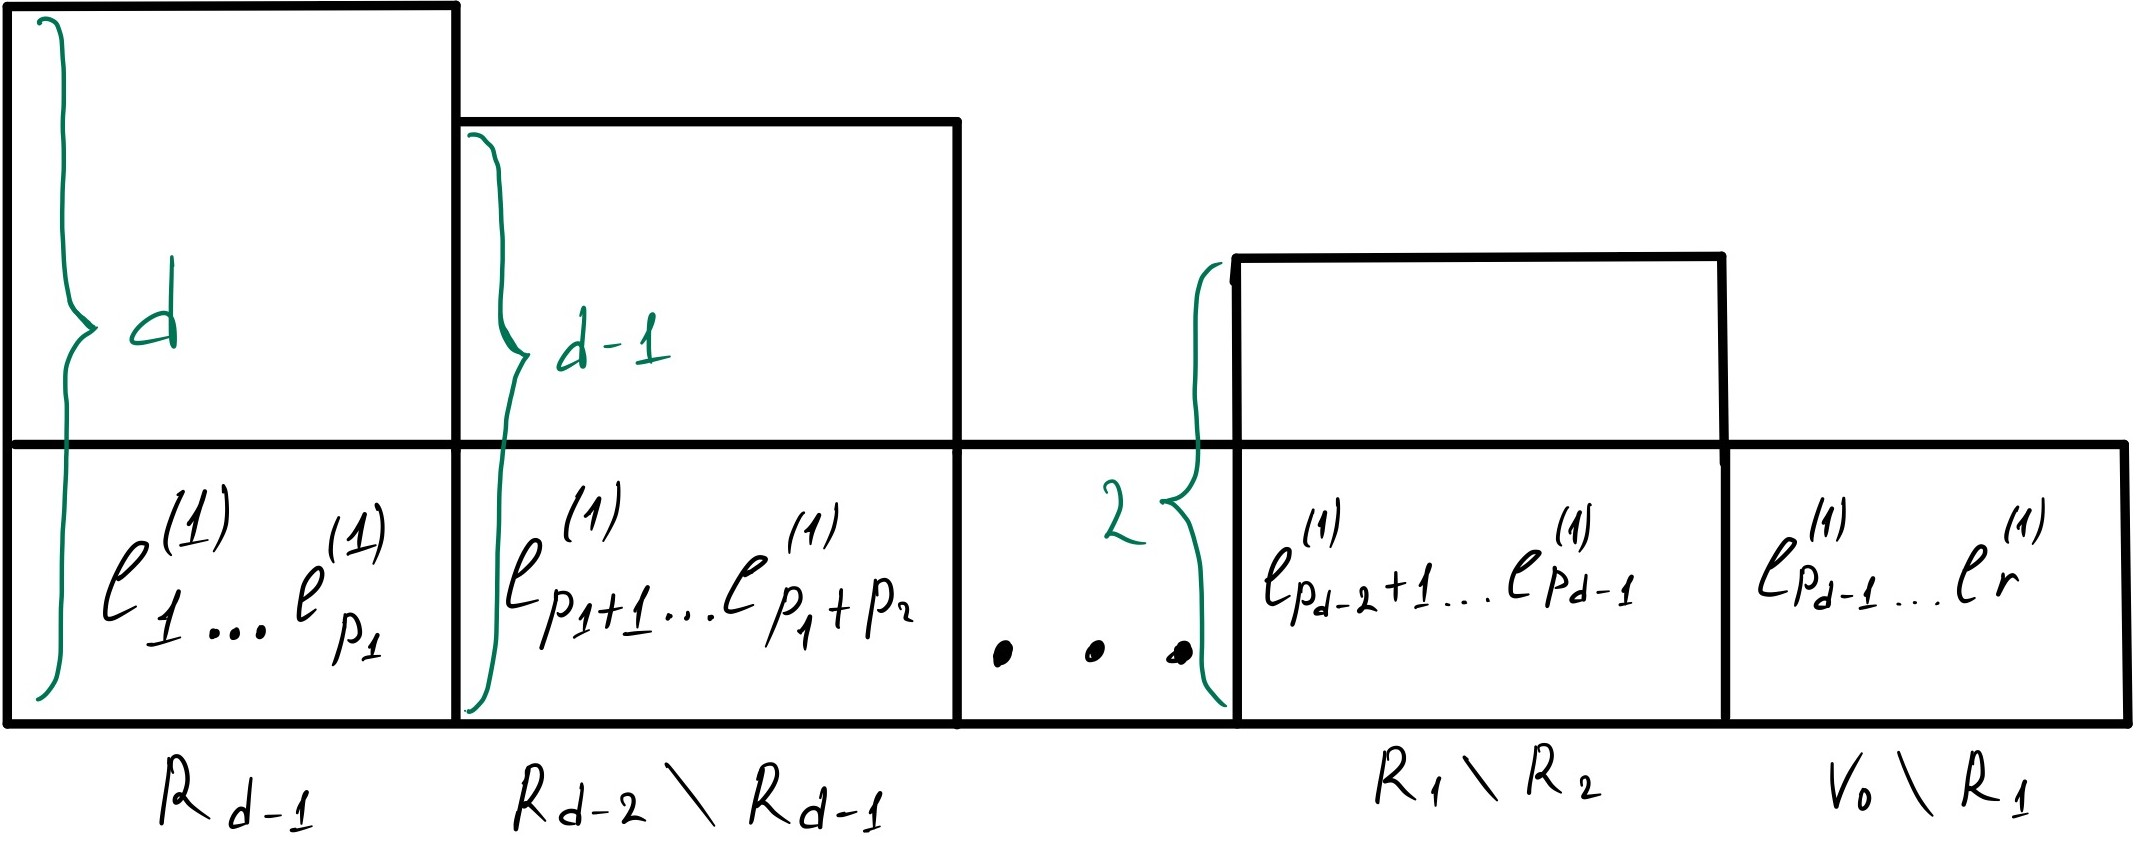
\includegraphics[scale = 0.22]{images/table1.JPG}\\
        Векторы $e_1^{(1)},...,e_{p_1}^{(1)} \in \text{Im}\psi
        ^{d-1} \Longrightarrow$ каждый из них имеет $(d-1)$
        присоединенный вектор.
        Например, $e_1^{(1)} = \psi(e_1^{(2)}),\ e_1^{(2)} =
        \psi(e_1^{(3)})$ и т.д.\\
        $e_1^{(p-2)} = \psi(e_1^{(p-1)}),$ т.о. векторы
        $\{e_1^{(p-1)}, e_1^{(p-2)},...,e_1^{(1)}\}$ образует 
        жорданову цепочку длины $p$. \\
        Эта цепочка имеет вид: $$\{e_1^{(p-1)}, \psi(e_1^
        {(p-1)}), \psi^2(e_1^{(p-1)}),...,\psi^{p-1}(e_1^
        {(p-1)}) = e_1^{(1)}\},\ \ \psi(e_1^{(1)}) = 0$$
        Таким образом, получаем некоторое количество
        жордановых цепочек длин $\leq d$. Векторы всех этих
        цепочек образуют базис в $V$.  
    \end{proof}
    \newpage
    \begin{lemma}
        Пусть есть $t$ жордановых цепочек $$\{a_1,\psi(a_1),...,
        \psi^{l_1 - 1}(a_1)\},\ \psi^{l_1}(a_1) = 0$$
        $$..............................................$$
        $$\{a_t,\psi(a_t),...,
        \psi^{l_t - 1}(a_t)\},\ \psi^{l_t}(a_t) = 0$$
        Причем конечные векторы этих цепочек ЛНЗ. Тогда 
        все векторы этих цепочек ЛНЗ. Кроме того, общее
        количество векторов в объединении цепочек равно 
        $dim V \Longrightarrow$ объединение всех цепочек из
        диаграммы -- базис пространства $V$.  
    \end{lemma}
    \begin{proof}
        Индукция по общему количеству векторов в цепочках.\\
        \textbf{База:} когда все цепочки имеют длину 1, т.е.
        $a_1,...,a_t$ -- собственные, ЛНЗ.
        \textbf{Предположение индукции:} $\exists$ хотя бы 
        одна цепочка длины $> 1$. \\
        Запишем линейную комбинацию: 
        $$\alpha_{11}a_1 + \alpha_{12}\psi(a_1) + ... +
        \alpha_{1,l_1}\psi^{l_1 - 1}(a_1) +...+ 
        \alpha_{t,1}a_t + \alpha_{t,2}\psi(a_t) +...+
        \alpha_{t,l_t}\psi^{l_t-1}(a_t) = 0$$
        Подействуем оператором $\psi$:
        $$\alpha_{11}\psi(a_1) + ... +
        \alpha_{1,l_1 - 1}\psi^{l_1 - 1}(a_1) +...+ 
        \alpha_{t,1}\psi(a_t) +...+
        \alpha_{t,l_t - 1}\psi^{l_t-1}(a_t) = 0$$ 
        Эти векторы принадлежат цепочкам длины $l_1 - 1,...,
        l_t - 1$ (либо какие-то\\ обратятся в 0)\\
        По предположению индукции
        $\alpha_{11} = ... = \alpha_{1,l_1 - 1} = ... = 
        \alpha_{t,1} = \alpha_{t,l_1 - 1} = 0 \Longrightarrow$
        $$\alpha_{a,l_1}\psi^{l_1 - 1}(a_1) +...+
        \alpha_{t,l_t}\psi^{l_t - 1}(a_t) = 0 \text{ ЛНЗ}
        \Longrightarrow$$ \text{остальные коэффициенты равны 0}
    \end{proof}
    $B$ -- нильпотентный оператор, $B^d = 0 \neq B^{d-1}
    \Longrightarrow $ максимальная длина (высота) жордановой
    цепочки равняется $d$.\\
    $R_i = \text{Im}B^i \cap \text{Ker}B,\ i = 1,..,d - 1$\\
    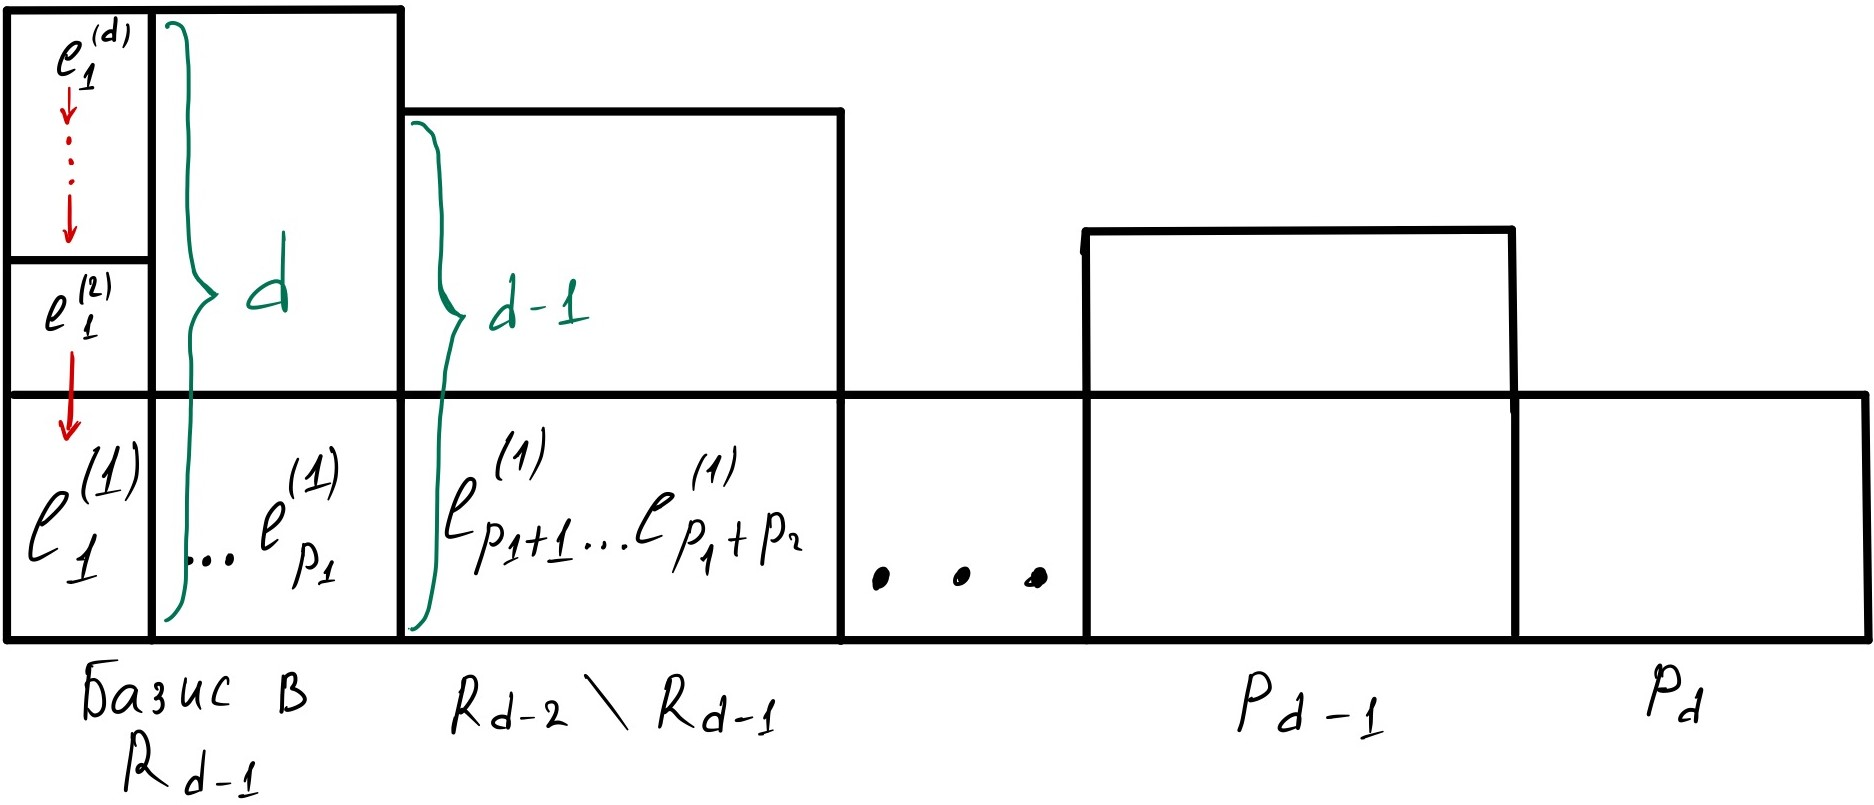
\includegraphics[scale = 0.25]{images/table2.JPG}\\
    Базис $\text{Ker}B = R_0$
    
    Общее число векторов в цепочках равно $\text{dim}V$
    (в котором действует $B$):
    $$dp_1 + (d-1)p_2 + ... + 2p_{d-1} + p_d =$$
    $$ =(p_1 +...+ p_d) + (p_1 + ... + p_{d-1}) +...+ (p_1 + p_2)
    + p_1 = $$
    $$= \text{dim}R_0 + \text{dim}R_1 +...+ \text{dim}R_{d-2}
    + \text{dim}R_{d-1}$$
    $$\sum\limits_{i=0}^{d-1}\text{dim}(\text{Im}B^i \cap 
    \text{Ker}B) = \sum\limits_{i=0}^{d-1}(\text{dimKer}B^
    {i+1} - \text{dimKer}B^i) =$$
    $$= \text{dimKer}B^d = \text{dim}V$$
    Нужно доказать, что $\text{dim}(\text{Im}B^i \cap \text{Ker}B) = 
    \text{dimKer}B^{i+1} - \text{dimKer}B^i$
    $$\text{Im}(B^i \cap \text{Ker}B) = \text{Ker}(B|_{\text{Im}B^i}) 
    \Longrightarrow$$ $$\text{dim}(\text{Im}B^i \cap \text{Ker}B) = 
    \text{dimIm}B^i - \text{dim}ImB^{i+1}=$$ $$= n - \text{dimKer}B^i
    - (n - \text{dimKer}B^{i+1})=$$ $$= \text{dimKer}B^{i+1} - 
    \text{dimKer}B^i$$$$
    \text{dimKer}\varphi = \text{dim}V - \text{dimIm}\varphi \Longrightarrow \varphi = B|_{\text{Im}B^i}$$
    \begin{center}
        \textbf{Единственность жордановой формы} 
    \end{center}
    Если $A \sim \mathcal{J} $ и $A \sim \mathcal{J}'$,
    то $\mathcal{J} $ и $\mathcal{J} '$ могут отличаться
    только упорядочиваниями жордановых клеток.\\
    Нужно доказать, что $\forall$ собственного значения $
    \lambda_j\ \exists m: 1 \leq m \leq d_j,\ N(m,\lambda_j)$  
    опеределено по $A$ единственным образом.\\
    Рассмотрим оператор $B = A - \lambda_j E$, достаточно
    для матрицы $B$ доказать единственность $N(m, 0):$
    $$N(m,0) = \text{dim}R_{m-1} - \text{dim}R_m = $$
    $$=(\text{dimKer}B^m - \text{dimKer}B^{m-1}) - 
    (\text{dimKer}B^{m+1} - \text{dimKer}B^m) = $$
    $$ = 2\text{dimKer}B^m - \text{dimKer}B^{m-1} - \text{dimKer}B^{m+1} =$$
    $$ =2(n - rkB^m) - (n - rkB^{m-1}) - (n - rkB^{m+1}) =$$
    $$=rkB^{m-1} - 2rkB^{m} + rkB^{m+1}$$
    Эти ранги не зависят от базиса.
    \newpage
    \textbf{Доказательство Теоремы Жордана в общем случае:}\\
    Пусть $\varphi: V \longmapsto V,\ A_\varphi$ -- его 
    матрица, $\chi_\varphi(t) = (\lambda_1 - t)^{k_1}\cdot...
    \cdot (\lambda_s - t)^{k_s},\ (\lambda_i \in F)$
    Тогда $V = \overset{s}{\underset{i=1}{\oplus}}\mathcal{K}_{\lambda_i},\  \mathcal{K}_{\lambda_i} = \text{Ker}(    
    \varphi - \lambda_i \varepsilon)^{k_i}$-- корневые
    подпространства.\\
    В базисе, согласованном с разложением,
    $$\begin{pmatrix}
        \underline{A_1\vline} & \null & \null & \null\\
        \null  & |\overline{\underline{A_2}}| & \null & \null\\
        \null & \null & \ddots & \null\\
        \null & \null & \null & \overline{|A_s} 
    \end{pmatrix}$$
    $\forall i = 1,...,s,\ A_i = A_{\varphi|_{\mathcal{K}
    (\lambda_i)}}$ имеет единственное собственное значение 
    $\lambda_i.$\\ Оператор $(\varphi - \lambda_i \varepsilon)$
    -- нильпотентный оператор $\Longrightarrow $ для него,
    по Теореме для нильпотентных операторов $\exists$ базис
    в $\mathcal{K}(\lambda_i)$  из жордановых цепочек.
    Тогда объединение базисов всех подпространств нужный базис.

    \begin{theorem}
        Пусть $\chi_A(t) = (-1)^n \prod\limits_{i=1}^{s}(t - 
        \lambda_i)^{k_i},\ d_i $--максимальный размер 
        жордановой клетки, отвечающей корню $\lambda_i$,
        тогда $\mu_A(t) = \prod\limits_{i=1}^{s}(t - \lambda_i)^
        {d_i}$ -- минимальный многочлен.  
    \end{theorem}
    \begin{proof}
        $\\$ Если $p(t)$ -- аннулирующий многочлен для $\varphi$
        (для матрицы $A$), тогда $\forall i\ p(\lambda_i) = 0$,
        если $x_i \neq 0:\ \varphi(x_i) = \lambda_i x_i$,
        то $$p(\varphi(x_i)) = p(\lambda_i)\underbrace{x_i}_
        {\neq 0} = 0 \Longrightarrow p(\lambda_i) = 0$$
        Для одной жордановой клетки $\mathcal{J}_m(\lambda_i)\
        (1 \neq m \neq d_i)$ 
        $$A - \lambda_i E = \begin{pmatrix}
        0 & 1 & \null & 0\\
        \null & \ddots & \ddots &  & \null\\
        \null & \null& \ddots & 1\\
        \null & \null & \null & 0
        \end{pmatrix} \Longrightarrow (A - \lambda_iE)^2 =
        \begin{pmatrix}
            0 & 0 & 1 & \null & 0\\
            \null & \ddots & \ddots & \ddots & \null\\
            \null &\null &\ddots &\ddots & 1\\
            \null &\null &\null &\ddots &0\\
            \null &\null &\null &\null &0
        \end{pmatrix}$$
        И т.д. $\Longrightarrow (A - \lambda_i E)^m = 0$\\
        Для $m = d_i$ наименьшая степень $q:\ (A - \lambda_i E)
        ^q = 0$ равна $d_i \Longrightarrow\\ \mu_A(t)\ \vdots
        \ (t - \lambda_i)^{d_i} \Longrightarrow \mu_A(t) = 
        \prod_{i=1}^{s}(t - \lambda_i)^{d_i}$
    \end{proof}
    \begin{consequense}
        $A_\varphi$ диагонализируема $\Longleftrightarrow$ 
        все характеристические корни имеют в $\mu_\varphi$
        кратность равную $1$.
    \end{consequense}
    \newpage
    \begin{center}
        \textbf{Некоторые применения жордановой формы} 
    \end{center}
    1. К решению СЛУ $AX = b,\ A_{(n\times n)}$\\
    Пусть уже найдена матрица $C$: $C^{-1}AC = \mathcal{J} =
    \begin{pmatrix}
        \mathcal{J}_1(\lambda_1) & \null & 0\\
        \null & \ddots & \null\\
        0 & \null & \mathcal{J}_l(\lambda_l) 
    \end{pmatrix}$\\
    Сделаем замену переменных: $$X = CY \Longrightarrow 
    A(CY) = b \Longrightarrow (C^{-1}AC)Y = C^{-1}b = b'$$
    Для каждой клетки $$\underset{\lambda \neq 0}{\begin{pmatrix}
        \lambda & 1 & \null & 0\\
        \null & \ddots & \ddots & \null\\
        \null & \null & \ddots & 1\\
        \null & \null & \null & \lambda
    \end{pmatrix}} \Longrightarrow 
    \begin{cases}
        \lambda y_1 + y_2 = b_1'\\
        \dots\\
        \lambda_n = b_n'
    \end{cases}$$ $\text{Легко дорешать, найдя } Y \text{
    найдем } X = CY$\\
    2. К вычислению функций от матрицы.\\
    $A_n^m,\ m \in \mathbb{N}$ $$
    A = CYC^{-1} = C \begin{pmatrix}
        \underline{\mathcal{J}_1}\vline & \null & 0\\
        \null & \ddots & \null\\
        0 & \null & \overline{\vline \mathcal{J}_l}
    \end{pmatrix}C^{-1} \Longrightarrow A^m = C\begin{pmatrix}
        \mathcal{J}_1 & \null & 0\\
        \null & \ddots & \null\\
        0 & \null & \mathcal{J}_l
    \end{pmatrix}C^{-1}$$
    Для одной клетки:
    $$\mathcal{J}_n(\lambda) = \begin{pmatrix}
        \lambda & 1 & \null & 0\\
        \null & \ddots & \ddots & \null\\
        \null & \null & \ddots & 1\\
        \null & \null & \null & \lambda
    \end{pmatrix} = \lambda E + 
    \begin{pmatrix}
        0 & 1 & \null & 0\\
        \null & \ddots & \ddots & \null\\
        \null & \null & \ddots & 1\\
        \null & \null & \null & 0
    \end{pmatrix} = \lambda E + B,\ B^n = 0 \neq B^{n-1}$$
    $$\Longrightarrow A^m = C\begin{pmatrix}
        \mathcal{J}_1^m & \null & 0\\
        \null & \ddots & \null\\
        0 & \null & \mathcal{J}_l^m
    \end{pmatrix}C^{-1},\ \mathcal{J}_n^m(\lambda) = 
    (\lambda E + B)^m 
    $$
    $\mathcal{J}_n^m(\lambda) = (\lambda E + B)^m = 
    \sum\limits_{k=0}^{m}C_m^k \lambda^k B^{m-k}$
    \newpage
    Для $m = \frac{1}{2}$ -- вычислить $\sqrt{A}$ (нужно,
    чтобы $\sqrt{\lambda_j}$ были определены)
    $$\underset{\lambda \neq 0}{\mathcal{J}_n(\lambda)}  = (\lambda E + B)^{\frac{1}{2}} =
    (\sqrt{\lambda}(E + \frac{1}{\lambda}B)^{\frac{1}{2}}) = 
    \sqrt{\lambda}(E + \frac{1}{2}X + C_{\frac{1}{2}}^2X^2 +...)$$
    $$(1 + x)^{\frac{1}{2}} = \sum\limits_{k=0}^{\infty}
    C_{\frac{1}{2}}^kx^k$$
    $$C_{\frac{1}{2}}^1 = \frac{1}{2},\ \ C_{\frac{1}{2}}^2 = 
    \frac{\frac{1}{2}(\frac{1}{2}-1)}{2!},...,C_{\frac{1}{2}}^k =
    \frac{\frac{1}{2}(\frac{1}{2}-1)...(\frac{1}{2}-k+1)}{k!}$$
    Экспонента:
    $e^A \overset{?!}{=} E + tA + t^2\frac{A}{2!}+...$
    $$A = C \mathcal{J}C^{-1} \Longrightarrow e^A = C
    \begin{pmatrix}
        e^{\mathcal{J}_1} & \null & 0\\
        \null & \ddots & \null\\
        0 & \null & e^{\mathcal{J}_l}
    \end{pmatrix}C^{-1}$$
    Для одной клетки порядка $n$:
    $$\mathcal{J}_n(\lambda) = \lambda E + B \Longrightarrow 
    e^{\mathcal{J}_n(\lambda)} = e^{\lambda E + B} = 
    e^{\lambda E}e^B = e^\lambda E e^B$$
    $$e^B = E + B + \frac{B^2}{2!} +...+ \frac{B^{n-1}}{(n-1)!} = 
    \begin{pmatrix}
        1 & 1 & \frac{1}{2!} & \dots & \frac{1}{(k-1)!}\\
        \null & 1 & 1 & \ddots & \vdots\\
        \null & \null & \null & \ddots & \frac{1}{2!}\\
        \hdotsfor{5}\\
        0 & \null & \null & \null & 1
    \end{pmatrix}$$
    $(e^{tA})' = Ae^{tA}$\\
    \underline{Формула:} $\text{det}(e^A) = e^{\text{tr}A}$
    \begin{theorem}
        Для любого линейного оператора $\varphi: V \longmapsto 
        V$ над $\mathbb{R}\ (\text{dim}V < \infty)$ существует
        одномерное или двумерное инвариантное подпространство.
    \end{theorem}
    \begin{proof}
        Пусть $\exists$ собственное значение $\lambda_0$,
        тогда и $\exists x_0 \in V,\ x_0 \neq 0$, т.ч. 
        $\varphi(x_0) = \lambda_0 x_0 \Longrightarrow 
        \langle x_0\rangle = U$ -- инвариантное подпространство.
        \\Комплексному корню отвечает двумерное инвариантное
        подпространство.\\ Допустим, что $\lambda_1 = 
        \alpha + i \beta \in \mathbb{C}$ -- корень $\chi_\varphi
        (\lambda) \Longrightarrow \overline{\lambda_1} = 
        \alpha - i \beta$ -- тоже корень $\Longrightarrow 
        \chi_\varphi(\lambda) = (\lambda - \lambda_1)
        (\lambda - \overline{\lambda_1})f(\lambda) = 
        (\lambda^2 - 2\alpha \lambda + (\alpha^2 + \beta^2))f(t),
        \ f(\lambda) \in \mathbb{R}[\lambda]$\\
        $\varphi$ с помощью (вещественной) матрицы $A_\varphi$
        действует в $\mathbb{R}^n:\\ \forall x \in \mathbb{R},\
        X \longmapsto A_\varphi X$\\
        Рассмотрим оператор $\varphi$ в $\mathbb{C}^n$    
        по формуле: $\forall Z \longmapsto A_\varphi Z$\\
        В $\mathbb{C}^n\ \exists$ вектор $Z_1:\ 
        A_\varphi Z_1 = \lambda_1 Z_1$\\
        $Z_1 = X_1 + iY_1,\ X_1, Y_1 \in \mathbb{R}^n\\ 
        A_\varphi X_1 + i A_\varphi Y_1 = 
        (\alpha X_1 - \beta Y_1) + i(\beta X_1 + \alpha Y_1)
        \Longrightarrow \begin{cases}
            A_\varphi X_1 = \alpha X_1 - \beta Y_1\\
            A_\varphi Y_1 = \beta X_1 + \alpha Y_1
        \end{cases} \Longrightarrow U = \langle X_1, Y_1
        \rangle \subset \mathbb{R}^n$ 
        -- двумерное инвариантное подпространство для $\varphi$.\\
        Допустим, что $Y_1 = \mu X_1 \Longrightarrow A_\varphi
        X_1 = (\alpha - \beta \mu)X_1 \Longrightarrow 
        X_1 \text{ -- собственный вектор.}\\
        \Longrightarrow X_1,\ Y_1$ -- ЛНЗ, $\text{dim}U = 2$  

    \end{proof}
    \begin{center}
        \begin{Large}
            \textbf{Глава III. Билинейные и квадратичные
            функции. Пространства с формами.}

            \textbf{\S 1. Билинейные функции.} 
        \end{Large}
    \end{center}

    \begin{definition}
        Функция $f:\ V\times V \longmapsto F$ называется
        билинейной, если:

        $1.\ f(\alpha_1 x_1 + \alpha_2 x_2, y) = \alpha_1
        f(x_1, y) + \alpha_2f(x_2, y),\ \forall x_1,x_2,y \in
        V,\ \alpha_1, \alpha_2 \in F$
        
        $2.$ По $y$.  
    \end{definition}

    \textbf{Примеры:}

    1. $V = R[a,b]$
    $$(f(x), g(x)) \longmapsto \int\limits_{a}^{b} f(x)g(x)dx =
    \int\limits_{a}^{b} g(x)f(x)dx \text{-- симметричная}$$

    2. $V = M_n(F)$
    $$f_1(X, Y) = \text{tr}(XY),\ f_2(X, Y) = \text{tr}(XY^T)$$
    Выражение $f(x,y)$ в координатах.\\ Пусть $e$ -- базис в $V$,
    $x = \sum\limits_{i=1}^{n} x_ie_i,\ y = \sum\limits_{j=1}
    ^{n} y_je_j \Longrightarrow$ $$f(x, y) = f(\sum\limits_{i=1}
    ^{n} x_ie_i ,\sum\limits_{j=1}^{n} y_je_j) = 
    \sum\limits_{i, j} \underbrace{f(e_ie_j)}_{f_{ij}}x_iy_j
    \text{ -- билинейная форма. (1)}$$

    \underline{Обозначение:} $B_e = (f_{ij})$ -- матрица
    билинейной формы $f(x,y)$ в базисе $e$.
    
    Выражение (1) можно записать в виде $f(x,y) = X^TB_eY$ (2).
    
    $\\$\textbf{Изменение матрицы билинейной формы при замене базиса:}\\
    Пусть $e' = eC_{e \to e'}$, тогда $X = CX',\ Y = CY'$ 
    подставим в (2).\\
    $X^TB_eY = (CX')^TB_e(CY') = (X')^T(C^TB_eC)Y' 
    \overset{?!}{=} (X')^TB_{e'}Y',\ \forall X', Y' \in F^n$
    Если $X'  =E_i,\ Y' = E_j$, то $(X')^TDY' = d_{ij},\ 
    \forall i,j \Longrightarrow B_{e'} = C^TB_eC\ (3)$

    \begin{consequense}
        1. $\text{rk}B' = \text{rk}B$, т.к. $|C| \neq 0$ 
        
        $\tab[2.2cm]$ 2. $|B'| = |B||C|^2$\\
        Если $F = \mathbb{R} \text{ и } |B| \neq 0$, то
        $|B'|$ и $|B|$ имеют одинаковый знак.
    \end{consequense}

    В силу следствия 1, $\text{rk}B$ можно называть рангом
    билинейной функции\\ $f(x,y),\ \text{rk}f$

    Назовем левым ядром билинейной функции $f(x,y):$
    $$\text{Ker}_{\text{л}} f = \{x \in V:\ f(x,y) = 0,\forall
    y \in V\}$$
    $$x \in \text{Ker}_{\text{л}} f \Longleftrightarrow 
    \begin{cases}
        f(x,e_1) = 0\\
        ...\\
        f(x,e_n) = 0
    \end{cases} - \text{ОСЛУ с матрицей }B$$
    Число ЛНЗ решений равно $n - \text{rk}B = n - \text{rk}f$. 
    
    \begin{definition}
        $f(x,y)$ \textit{симметричная}, если $\forall x,y \in V:
        \ f(x,y) = f(y,x)$  
    \end{definition}
    \begin{definition}
        $g(x,y)$ \textit{кососимметричная}, если $\forall x,y
        \in V:\ f(x,y) = -f(y,x)$  
    \end{definition}
    \begin{theorem}
        Если char$F \neq 2$, то любая билинейная функция 
        $f(x,y)$ единственным образом представляется в виде:
        $f(x,y) = f_+(x,y) + f_-(x,y)$
    \end{theorem}
    \begin{proof}
        $$\begin{cases}
            f(x,y) = f_+(x,y) + f_-(x,y)\\
            f(x,y) = f_+(x,y) - f_-(x,y)
        \end{cases}$$
        $$f_+(x,y) = \frac{f(x, y) + f(y,x)}{2},\ 
        \ f_- (x,y) = \frac{f(x,y) - f(y,x)}{2}$$
    \end{proof}
    \begin{center}
        \begin{Large}
            \textbf{\S 2. Квадратичные функции (формы).} 
        \end{Large}
    \end{center}
    \begin{definition}
        Пусть $f(x,y)$ -- билинейная функция на $V$. Тогда 
        функция\\ $k_f(x):= f(x,x),\ \forall x \in V$ 
        называется \textit{квадратичной функцией, 
        порожденной билинейной функцией} $f$, если $k_f(x)
        \not\equiv 0$.
    \end{definition}
    Обратим внимание, что если $f(x,y) = f_+(x,y) + f_-(x,y)$, то 
    $$f(x,x) = f_+(x,x) + \underset{-f_-(x,x) = 0}{f_-(x,x)}
    ,\ \text{char}F \neq 2 \Longrightarrow$$ 
    $f \text{ и } f_+$ порождают одну и ту же функцию.

    \begin{theorem}
        Для любой квадратичной функции $k(x)$ существует
        единственная билинейная симметричная функция $f(x,y)$,
        т.ч. $f(x,x) = k(x)$  
    \end{theorem}
    \begin{proof}
        Пусть $f(x,y) = f(y,x)$\\
        Рассмотрим $k(x + y) = f(x + y, x + y) = f(x,x) + 
        f(x,y) + f(y,x) + f(y,y) = f(x,x) + 2f(x,y) + f(y,y)
        ,\ \forall x,y \in V \Longrightarrow f(x,y) = 
        \frac{k(x+y) - k(x) - k(y)}{2}$
    \end{proof}
    \underline{Координатная запись:} $$k(x) = X^TB_eX = \sum\limits_{i,j}
    b_{ij}x_ix_j = \sum\limits_{i,j} b_{ii}x_i^2 +
    2\sum\limits_{i < j} b_{ij}x_ix_j,\ b_{ij} = b_{ji},\
    \forall i,j,\ (2)$$
    Договоримся, что матрица квадратичной формы (2)
    совпадает с матрицей $B$.

    $$k(x_1,x_2) = 3x_1^2 - 4x_1x_2 + 25x_2^2, \tab[1cm]
    B \overset{?}{=} \begin{pmatrix}
        3 & 2\\-2 & 25
    \end{pmatrix}$$ 
    
    \begin{center}
        \textbf{Упрощение квадратичной формы}    
    \end{center}
    
    \underline{Термин:} Диагональная квадратичная форма:
    $$k(x) = \alpha_1x_1^2 +...+ \alpha_nx_n^2 = \alpha_1x_1^2
    +...+\alpha_rx_r^2$$
    (При подходящей нумерации переменных). 
    $(x = (x_1,...,x_n))$\\
    Если $\text{rk}f = rk = k = r \leq n$
    $$B = \begin{pmatrix}
        \alpha_1  & \null & \null & \null & & \null 0\\
        \null & \ddots & \null & \null & \null & \null\\
        \null & \null & \alpha_r & \null & \null & \null\\
        \null & \null & \null & 0 & \null & \null\\
        \null & \null & \null & \null & \ddots & \null\\
        0 & \null & \null & \null & \null & 0
    \end{pmatrix}
    $$ 
    

    \underline{Термин:} $(F = \mathbb{R})$
    $k(x)$ имеет канонический вид, если
    $$k(x) = \sum\limits_{i=1}^{p}x_i^2 - \sum\limits_
    {i=p+1}^{p+q}x_i^2,\ (p+q = \text{rk}\ k = r)$$
    Если $F = \mathbb{C}$, то канонический вид будет
    $$\sum\limits_{i=1}^{r}  x_i^2$$
    Над $\mathbb{R}$: замена $y_i = \sqrt{|\alpha_i|}x_i,\ 
    1 \leq i \leq r,\ y_i = x_i,\ i = r+1,...,n$\\
    Тогда $k(x)$ равен каноническому виду.\\
    Над $\mathbb{C}$: $\forall i = 1,...,r\ \ y_i =
     \sqrt{|\alpha_i|}x_i$
    \newpage
    \begin{center}
        \textbf{Алгоритм Лагранжа (метод выделения квадратов.)} 
    \end{center}

    Пусть $k(x_1,...,x_n) = b_{11}x_1^2 +...+ b_{nn}x_n^2 + 
    2b_{12}x_1x_2 +...+ 2b_{1n}x_1x_n \undermat{
    x_1\text{ не входит}}{+...}$\\
    Основной случай: $b_{11} \neq 0 \Longrightarrow$
    $$b_{11}(x_1^2 + 2x_1\sum\limits_{i=2}^{n}\frac{b_{1i}}
    {b_{11}} x_i)  +...= 
    b_{11}(x_1^2 + 2x_1(\sum\limits_{i=2}^{n} 
    \frac{b_{1i}}{b_{11}} x_i) + (\sum\limits_{i=2}^{n}
    \frac{b_{1i}}{b_{11}} x_i)^2) -$$ 
    $$\underbrace{- \frac{1}{b_{11}}
    (\sum\limits_{i=2}^{n} b_{1i}x_i)^2 + 2 \sum\limits_
    {1 < i < j} b_{ij}x_ix_j}_{k_1(x_2,...,x_n)} = 
    b_{11}(x_1 + \sum\limits_{i=2}^{n} \frac{b_{1i}x_i}{b_{11}})
    ^2 + k_1(x_2,...,x_n)$$ 
    Замена: $y_1 = x_1 + \sum\limits_{i=2}^{n} \frac{b_{1i}}
    {b_{11}}x_i$, остальные пока не заменяем.
    
    Особый случай: $b_{ii} = 0,\ \forall i = 1,...,n$\\
    Т.к. $k(x) \not\equiv 0 \Longrightarrow \exists i,j:\ 
    b_{ij} \neq 0$\\
    Подготовительная замена:
    $$\begin{cases}
        x_i = x_i' - x_j'\\
        x_j = x_i' + x_j'
    \end{cases} \Longrightarrow 2b_{ij}x_ix_j = 
    2b_{ij}((x_i')^2 - (x_j')^2) \Longrightarrow \text{ перейти 
    к основ. случаю}$$
    Заммечание: можно сделать такую замену:
    $\begin{cases}
        x_i = \tilde{x}_i + \tilde{x}_j\\
        x_j = \tilde{x}_j
    \end{cases}$
    
    \begin{center}
        \textbf{Закон инерции для квадратичных форм над $\mathbb{R}$} 
    \end{center}
    Если в некотором базисе $e$ квадратичная форма $k(x_1,...,
    x_n) = \sum\limits_{i=1}^{p}x_i^2 - \sum\limits_{i=p+1}^{p+q}
    x_i^2$,\\ а в базисе $f$: $k(y_1,...,y_n) = \sum\limits_
    {i=1}^{s}y_i^2 - \sum\limits_{i=s+1}^{s+t}y_i^2$,
    то $p = s,\ q = t$
    \begin{remark}
        $p+q = s+t = \text{rk}\ k$, так что достаточно доказать,
        что $p = s$  
    \end{remark}   
    \begin{proof}
        От противного. Допустим, что $p>s$\\
        Рассмотрим два подпространства:
        $L_1 = \langle e_1,...,e_p\rangle$, $L_2 = \langle f_{s
        +1},...,f_n\rangle$\\
        Обратим внимание, что если $x \in L_1,\ x \neq 0,$
        то $k(x) > 0;\ \forall y \in L_2:\ k(y) \leq 0$
        $$\text{dim}L_1 + \text{dim}L_2 = p + (n-s) = n +
        (p-s) > n\Longrightarrow$$ $$L_1 \cap L_2 \neq \{0\}:\ 
        n \geq \text{dim}(L_1 + L_2) = \underbrace{\text{dim}
        L_1 + \text{dim}L_2}_{> n} - dim(L_1 \cap L_2)
        \Longrightarrow$$
        $$dim(L_1 \cap L_2) > 0$$
        \newpage
        Но $\forall v \in L_1 \cap L_2,\ v \neq 0:\ 
        k(v) > 0$ и $k(v) < 0$ -- противоречие $\Longrightarrow$
        \begin{flushright}
            $p > s$ не может быть.
        \end{flushright}
        Доупустим, что $s > p$, тогда рассмотрим
        $L_1' = \langle e_{p+1},...,e_n\rangle$, 
        $L_2' = \langle f_{1},...,f_s\rangle$
        $$n - p + s = n + (s - p) > n \Longrightarrow
        L_1' \cap L_2' \neq \{0\}$$
        $$\forall u \in L_1' \cap L_2',\ u \neq 0:\ k(u) > 0,\ k(u) < 0 
        \Longrightarrow$$ $$p = s \Longrightarrow q = t$$

    \end{proof}
    \begin{center}
        \begin{Large}
            \textbf{\S 3. Знакоопределенные квадратичные формы.} 
        \end{Large}
    \end{center}
    Пусть $k(x)$ -- квадратичная форма на пр-ве $V$
    над полем $F,\ \text{char}F \neq 2$.\\
    $f(x,y)$ -- полярная билинейная форма, $f(x,y) = f(y,x),\ 
    f(x,x) \equiv k(x)$.\\
    Скажем, что $u \bot v$, если $f(u,v) = 0$.\\
    Скажем, что базис $e_1,...,e_n$ в пространстве $V$ 
    ортогональный,
    \begin{flushright}
        если $f(e_i, e_j) = 0,\ \forall i \neq j$
    \end{flushright} 
    \begin{remark}
        Форма является симметрической $\Longleftrightarrow $
        ее матрица является\\ $\tab[3.15cm]$симметрической. 
    \end{remark}
    Если $B = \begin{pmatrix}
        b_{11} & \dots & b_{ii} & \vline & \dots & b_{1n}\\
        \vdots & \null & \vdots & \vline & \null &  \vdots\\
        b_{1i} & \dots & b_{ii} & \vline & \dots & b_{in}\\
        \cmidrule{1-4}
        % \hline
        \vdots & \null & \vdots & \null & \null &  \vdots\\
        b_{1n} & \dots & b_{in} & \null & \dots & b_{nn}\\
    \end{pmatrix}$, то $B = B^T$
    \begin{flushright}
        Главный угловой минор порядка $i$
        матрицы $B$:
        $\begin{vmatrix}
            b_{11} & \dots & b_{1i}\\
            \vdots & \null & \vdots\\
            b_{1i} & \dots & b_{ii}
        \end{vmatrix}$  
    \end{flushright}

    \textbf{Теорема Якоби.} Пусть $B$ -- матрица квадратичной
    формы $k(x)$ (в данном базисе $e$) и все главные миноры
    этой матрицы отличны от 0: $\Delta_1\Delta_2\cdot...
    \cdot \Delta_n \neq 0$. Тогда в пространстве $V$ 
    существует базис $e' = \{e_1',...,e_n'\}$, в котором 
    $$k = \frac{\Delta_1}{\Delta_0}y_1^2 + 
    \frac{\Delta_2}{\Delta_1}y_2^2 +...+
    \frac{\Delta_n}{\Delta_{n-1}}y_n^2\ (\text{по 
    договренности }\Delta_0 = 1)$$
    \begin{proof}
        Процесс ортогонализации -- последовательное построение
        \\векторов, начиная с $e_1' = e_1$, чтобы векторы были 
        ортогональными друг другу.

        Это включает требования: $\forall m \geq 2$\\
        $1.\ f(e_i', e_j') = 0,\ \forall i \neq j,\ 
        1 \leq i,j \leq m$\\
        $2.\ \langle e_1',...,e_m'\rangle = \langle e_1,...,
        e_m\rangle$

        Берем $e_1' = e_1,\ e_2'$ ищем в виде $e_2' = e_2 - 
        \lambda e_1'$
        $$f(e_2',e_1') = f(e_2 - \lambda e_1', e_1') = 
        f(e_2, e_1') - \lambda f(e_1',e_1') = 
        f(e_2,e_1) - \lambda k(e_1')$$ 
        $$\lambda = \frac{f(e_2,e_1)}{k(e_1')},\ 
        k(e_2') = f(e_2 - \lambda e_1', e_2 - \lambda e_1') =
        f(e_2,e_2) - 2\lambda f(e_2,e_1') + \lambda^2 k(e_1')$$
        Матрица перехода от $e_1, e_2 \longmapsto e_1' e_2'$\\
        $C_2 = \begin{pmatrix}
            1 & -\lambda\\
            0 & 1
        \end{pmatrix}$
        $\tab[2cm]\Delta_2' = k(e_1')k(e_2') = \Delta_2 
        \Longrightarrow k(e_2') = \frac{\Delta_2}{\Delta_1}$
        $$B' = \begin{pmatrix}
            f(e_1', e_1') & f(e_1', e_2') & \dots\\
            f(e_2', e_1') & f(e_2', e_2') & \dots\\
            \dots & \dots & \dots
        \end{pmatrix} \sim
        \begin{pmatrix}
            f(e_1') & 0 & \dots\\
            0 & f(e_2') & \dots\\
            \dots & \dots & \dots
        \end{pmatrix}$$
        $$B' =\begin{pmatrix}
            B_2' \vline & \null & \null\\\cmidrule{1-1}
            \null & \ddots & \null
        \end{pmatrix}\tab[1cm]
        B_2' = C_2^TB_2C_2,\ |B_2'| = \Delta_2' = |C_2|^2|B_2|
        = |B_2| = \Delta_2$$
        
        Рекурсия. Пусть векторы $e_1,...,e_{m-1}\ (m \geq 2)$
        уже построены, исходя из условий (1), (2) процесса
        ортогонализации.
        Вектор $e_m'$ будем искать в виде:
        $$e_m' = e_m - \sum\limits_{i=1}^{m-1}\lambda_i e_i',
        \text{ чтобы } f(e_m', e_j') = 0,\ \forall j = 1,...,m-1$$
        $$f(e_m', e_j') = f(e_m - \sum\limits_{i=1}^{m-1}
        \lambda_ie_i', e_j') = f(e_m, e_j') - \sum\limits_{i=1}
        ^{m-1}\lambda_if(e_i', e_j') = 0$$
        $$f(e_i', e_j') = 0,\ i \neq 0 \Longrightarrow 
        \text{ останется } f(e_m, e_j') - \lambda_if(e_j',e_j') = 0$$
        
        Это можно проделать вплоть до $m = n \Longrightarrow $ 
        $\lambda_i = \frac{f(e_m,e_j')}{k(e_j')},\ 
        1\leq j \leq m-1 $

        Новая матрица: 
        $$B' = \begin{pmatrix}
            k(e_1')  & \null\\
            \null & \ddots & \null\\
            \null & \null& k(e_n')
        \end{pmatrix} = C^TBC \Longrightarrow |B'| = |C|^2
        |B| = |B| \text{ или } \Delta_n' = \Delta_n$$
        Тогда $\Delta_n' = k(e_1')\cdot...\cdot k(e_n') = 
        \Delta_n$
        
        Применим индукцию для $m \leq n-1 \Longrightarrow 
        k(e_1')\cdot...\cdot k(e_{n-1'}) = \Delta_{n-1}
        \Longrightarrow k(e_n') = \frac{\Delta_n}{\Delta_{n-1}} $

    \end{proof}
    \textbf{Следствия из теоремы Якоби:} (для $\Delta_1\cdot
    ...\cdot\Delta_n$, над $\mathbb{R}:\ \text{rk} = n,$)\\
    $p$ (положительный индекс инерции) равен числу сохранений
    знака,\\ а $q$ (отрицательный индекс инерции) -- числу 
    перемен знака в последовательности $\Delta_0,..., 
    \Delta_n$
    $$k(y_1,...,y_n) = \sum\limits_{m=1}^{n} \frac{\Delta_m}
    {\Delta_{m-1}}y_m^2 $$

    Квадратичная форма $k(x)$ является:
    \begin{itemize}
        \item Положительно определенной на $V$, если $\forall v 
        \neq 0,\ k(v) > 0$
        \item Отрицательно определенной, если $\forall v \neq 0,
        \ k(v) <0$    
        \item Неотрицательно опеределенная, если $\forall v 
        \neq 0,\ k(v) \geq 0$
        \item  Неположительно опеределенная, если $\forall v 
        \neq 0,\ k(v) \leq 0$
    \end{itemize}
    \begin{lemma}
        Квадратичная форма является:
        
        1. Положительно определенной $\Longleftrightarrow p = n,
        \ q = 0$
        
        2. Отрицательно определенной $\Longleftrightarrow p=0, 
        \ q= n$
        
        3. Неотрицательно определенной $\Longleftrightarrow q=0,
        \ p > 0$ 

        4. Неположительно определенной $\Longleftrightarrow  p 
        = 0,\ q > 0$ 

        5. Неопределенной $\Longleftrightarrow p > 0,\ q > 0$ 
    \end{lemma}
    \textbf{Критерий Сильвестра.} $k > 0 \Longleftrightarrow \Delta_1 > 0,...,\Delta_n > 0$\\
    $\tab[5.9cm]k < 0 \Longleftrightarrow (-1)^i \Delta_i > 0,\ \forall i = 1,...,n$ 
    \begin{proof}
        Докажем для $k > 0$, для $k < 0$ -- 
        аналогично.

        $\Longleftarrow$ Дано, что $\forall i,\ \Delta_i > 0
        \Longrightarrow k > 0$\\
        По теореме Якоби $\exists$ замена координат
        $X = CY$, что $k = \sum\limits_{i=1}^{n}
        \frac{\Delta_i}{\Delta_{i-1}}y_i^2$\\
        По условию, $\forall i,\ \frac{\Delta_i}{\Delta_{i-1}}
        > 0 \Longrightarrow p=n \Longrightarrow k > 0$

        $\Longrightarrow k > 0 \Longrightarrow $ все 
        $\Delta_i>0$\\
        Из условия $\Delta_n > 0$, т.к. $\underbrace{\Delta_n'}_
        {> 0} = \Delta_n|C|^2$, известно, что $p = n$\\
        $\forall i$ рассмотрим $k(y_1,...,y_i,0,...,0) \neq 0
        \Longrightarrow $ для нее $\Delta_i = |B_i|$ 
    \end{proof}
    \newpage
    \textbf{Примеры применения критерия Сильвестра}
    $$f(x,y) = f(x_0,y_0) + \frac{1}{2}d^2f(x_0,y_0) +
    o((\Delta x^2 + \Delta y^2))$$
    $(x_0,y_0)$ -- точка экстремума. $\Longrightarrow 
    f_x'(x_0, y_0) = f_y'(x_0, y_0) = 0$  
    $$d^2f(x_0, y_0) = f_{xx}''(M_0)(\Delta x)^2 + 
    2f_{xy}''(M_0)\Delta x \Delta y + f_{yy}''(M_0)(\Delta y)
    ^2$$
    $$\begin{vmatrix}
        f_{xx}'' & f_{xy}''\\
        f_{yx}'' & f_{yy}''
    \end{vmatrix}\tab[1cm] (x_0,y_0) - \text{точка минимума} 
    \Longleftrightarrow d^2f(x_0,y_0) >0$$

    \begin{center}\begin{Large}
        \textbf{\S 4. Евклидовы пространства.}
    \end{Large}\end{center}
    \begin{definition}
        Пространство $\mathcal{E}$ над $\mathbb{R}$ называется
        евклидовым, если на $\mathcal{E}$\\ задано скалярное 
        произведение
        $(x,y)$ -- симметричная билинейная форма, т.ч. 
        соотвествующая квадратичная функция $(x,x) > 0,\ 
        x \in \mathcal{E},\ x \neq 0$. (В геометрии, 
        dim $\varepsilon < \infty$)
    \end{definition}
    \textbf{Примеры:}

    1. В $C[a,b],\ (f(x), g(x)) = \int_{a}^{b}f(x)g(x)dx$
    $$(f,f) = \int_{a}^{b} f^2(x)dx > 0,\ \text{где } f \not
    \equiv 0$$

    2. В $M_n(\mathbb{R})$\\
    $(X,Y) = tr(XY^T)$\\$(X,X) = tr(XX^T) = \sum\limits_{i,j=1}^
    {n} x_{ij}^2$\\
    $(XX^T)_{ii} = (x_{i1}\cdot...\cdot x_{in})\begin{pmatrix}
        x_{i1}\\\vdots\\x_{in}
    \end{pmatrix} = x_{i1}^2 +...+ x_{in}^2$
    \begin{center}
        \textbf{Неравенство Коши-Буняковского-Шварца.} 
    \end{center}
    Пусть $\mathcal{E}$ -- евклидово пространство, тогда
    $\forall x,y \in \mathcal{E} \ |(x,y)| \leq |x||y|\tab[1cm]
    (1)$\\  
    Более того, если выполняется равенство, то $x\ ||\ y$.
    \begin{proof}
        Если $x = 0 \text{ или } y = 0$, то $(1)$ имеет вид 
        $0 = 0$.\\
        Можно считать, что $x \neq 0,\ y \neq 0$.\\
        Рассмотрим функцию:
        $$f(t) = (y - tx, y - tx) = (y,y) - 2t(x,y) + t^2(x,x),
        \ \forall t \in \mathbb{R} \Longleftrightarrow  $$
        $$\frac{\Delta}{4} = (x,y)^2  - |x|^2|y|^2 \leq 0
        \Longrightarrow (x,y)^2 \leq |x|^2|y|^2 
        \Longleftrightarrow $$
        $$|(x,y)| \leq |x||y|$$
        Равенство означает, что $$\Delta = 0 \Longrightarrow 
        \exists !\ t = t_0:\ (y - t_0x, y - t_0x) = 0
        \Longrightarrow y = t_0x \Longrightarrow y\ ||\ x.$$ 
    \end{proof}
    
    \begin{consequense}
        $\forall x,y \in \mathcal{E}:\ |x + y| \leq |x| + |y|
        \ \ \  (2)$
    \end{consequense}
    \begin{proof}
        $(2) \Longleftrightarrow |x + y|^2 \leq |x|^2 + 2(x,y)
        + |y|^2 \leq |x|^2 + 2|x||y| + |y|^2$ 

    \end{proof}
    \begin{definition}
        Если $x \neq 0,\ y \neq 0$, то опеределим угол
        $\alpha$ между $x \text{ и } y:$
        $$\cos \alpha = \frac{(x,y)}{|x||y|}\ (3),\ \alpha = 
        \arccos \frac{(x,y)}{|x||y|} $$
    \end{definition}
    \begin{definition}
        Векторы $a_1,...,a_m \in \mathcal{E}$ -- ортогональная
        система, если\\ $(a_i, a_j) = 0,\ \forall i \neq j$ и $
        (a_i,a_i) = 1,\forall i = 1,...,m.$ 
    \end{definition}
    \begin{subtheorem}
        Ортогональная система ненулевых векторов ЛНЗ.
    \end{subtheorem}
    \begin{proof}
        Пусть $\lambda_1a_1 + ... + \lambda_ma_m = 0\ |\cdot 
        a_i \Longrightarrow $
        $$\lambda_1\underbrace{(a_1,a_i)}_{ = 0} + ... + 
        \lambda_i(a_i,a_i) +...+ 
        \lambda_m\underbrace{(a_m,a_i)}_{= 0} = 0 
        \Longrightarrow $$
        $$\lambda_i(a_i,a_i) = 0 \Longrightarrow \lambda_i = 0,
        \ \forall i = 1,...,m.$$
    \end{proof}
    \begin{theorem}
        В конечномерном евклидовом пространстве существует
        ортогональный (более сильное утверждение: 
        ортонормированный) базис.
    \end{theorem}
    (Существование ортогонального базиса было доказано
    при доказательстве теоремы Якоби -- процесс 
    ортогонализации).

    Если $a_1,...,a_m$ -- ортогональный базис, то
    $\frac{a_1}{|a_1|},...,\frac{a_n}{|a_n|}$ -- 
    ортогональный базис.

    Запись скалярного произведения $(x,y)$ в координатах:\\
    пусть $e = \{e_1,...,e_n\}$ -- базис в $\mathcal{E}$
    $$(\sum\limits_{i=1}^{n} x_ie_i,\ 
    \sum\limits_{j=1}^{n} y_je_j) = 
    \sum\limits_{i,j=1}^{n} (e_i,e_j)x_iy_i = X^TG_eY\tab[1cm] (4)$$
    Обознач. $G_e = ((e_i,e_j))$ -- матрица Грама базиса
    $e_1,...,e_n$, она симметрическая, причем положительно
    определенная.
    $$G \text{ явл. матрицей Грама} \Longleftrightarrow 
    \begin{cases}
        G^T = G\\ \Delta_1,...,\Delta_n > 0
    \end{cases}$$
    Если базис ортонормированный то $G_e = E$, тогда
    $(x,y) = \sum\limits_{i=1}^{n} x_iy_i$\\
    Разложение любого вектора $x$ по ортонормированному 
    базису $e$: $$x = \sum\limits_{i=1}^{n}(x,e_i)e_i$$
    \begin{center}
        \begin{Large}
            \textbf{\S 5 Ортогональное дополнение.}         
        \end{Large}
    \end{center}
    \begin{definition}
        Пусть $\mathcal{E}$ -- евклидово пространство,
        $\varnothing \neq U \subseteq \mathcal{E}$, тогда
        ортогональное дополонение к $U$ в $\mathcal{E}$ -- это 
        подмножество $U^\perp = \{y \in \mathcal{E}|\ 
        (x,y) = 0,\ \forall x \in U\}$ 
    \end{definition}
    Заметим, что если $U \neq 0,$ то $U$ подпространство в
    $\mathcal{E}$:
    $$0\in U^\perp,\ (x,y_1) = 0,\ (x,y_2) = 0 
    \Longrightarrow $$
    $$(x,\alpha_1y_1 + \alpha_2y_2) = \alpha_1\underbrace{(x
    ,y_1)}_{= 0} + \alpha_2\underbrace{(x,y_2)}_{= 0} = 0\\
    \Longrightarrow \alpha_1y_1 + \alpha_2y_2 \in U^\perp$$
    \begin{theorem}
        Если dim $\mathcal{E} = n,\ U \subseteq \mathcal{E}$ --
        подпространство в $\mathcal{E}$, то
        
        1. $dim U + dim U^\perp = dim\mathcal{E} = n$
       
        2. $\mathcal{E} = U \oplus U^\perp$ 
    \end{theorem}
    \begin{proof}
        $U \cap U^\perp = \{0\}$: если $v \in U \cap U^\perp
        \Longrightarrow (v,v) = 0 \Longrightarrow v = 0$

        Выберем базис в $U:\ e_1,...,e_m\ (dimU = m,\ 
        0 < m < n).$
        $$y \in U^\perp \Longleftrightarrow (y, e_i) = 0,
        \ \forall 1 \leq i \leq m$$
        $\Longrightarrow $ по определению.\\
        $\Longleftarrow$ если $(y,e_i) = 0,\ \forall i = 
        1,...,m$ и $\sum\limits_{i=1}^{m} x_ie_i 
        \Longrightarrow (x,y) = \sum\limits_{i=1}^{m}
        x_i(e_i,y) = 0$

        Получается, что $U^\perp$ -- подпространство решений
        ОСЛУ:
        $$\begin{cases}
            (e_1,y) = 0\\\dots\\(e_m,y) = 0
        \end{cases} \Longrightarrow dimU^\perp = n - m
        \Longrightarrow dimU^\perp + dimU = n \Longrightarrow \mathcal{E} = U \oplus U\perp$$ 
        Это означает, что объединив О.Н.Б. пространства $U$
        и О.Н.Б. пространства $U^\perp$, получим О.Н.Б в 
        $\mathcal{E}$ (О.Н.Б. - ортонормированный базис).   
    \end{proof}
    \begin{center}
        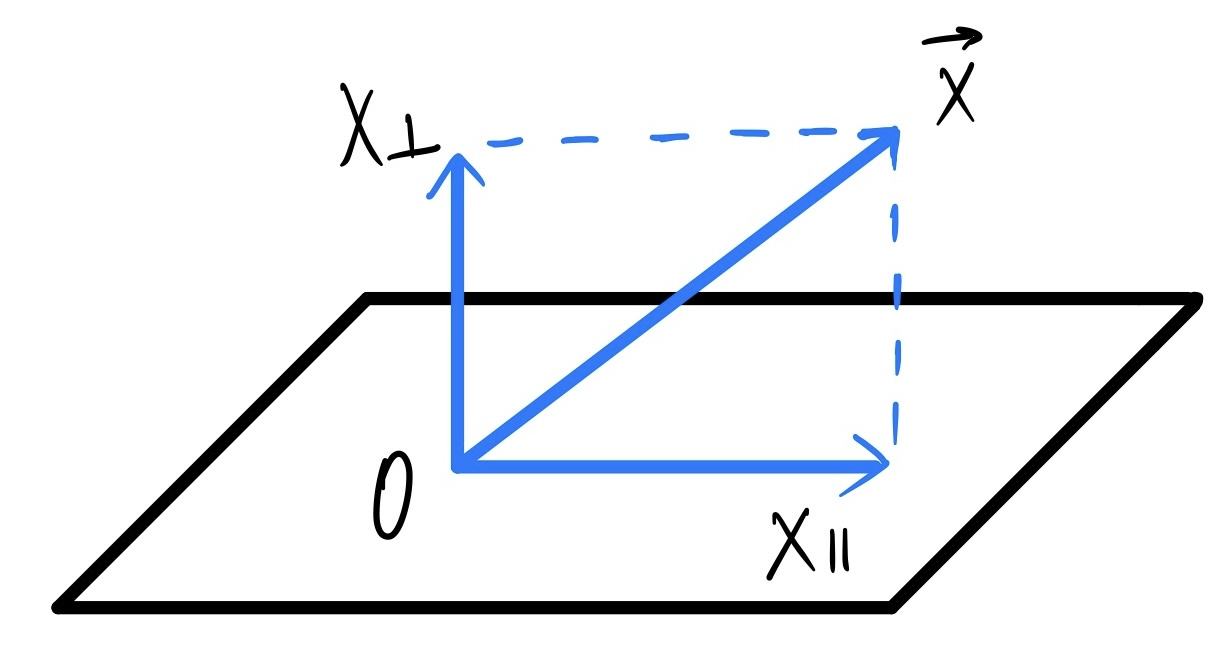
\includegraphics[scale = 0.22]{images/picture.JPG}    
    \end{center}

    $x = x_{||} + x_\perp,\ x_{||} \in U,\ x_\perp \in 
    U^\perp$

    $x_{||}$ -- ортогональная проекция вектора $x$ на $U$.

    $x_\perp$ -- ортогональная проекция вектора $x$ на
    $U^\perp$.

    Конкретно разложение вектора $x \in \mathcal{E} $ на 
    сумму проекции и составляющей. 

    \underline{1 способ.} Выбрать О.Н.Б. в $\varepsilon, \
    \underbrace{e_1,...,e_m}_{\text{О.Н.Б в } U},
    \underbrace{e_{m+1},...,e_n}_{\text{О.Н.Б в } U^\perp}$
    $$\forall x = \underbrace{\sum\limits_{i=1}^{m}(x,e_i)e_i}
    _{x_{||}} + \underbrace{\sum\limits_{i=m+1}^{n}(x, e_i)e_i}_
    {x_\perp}$$

    \underline{2 способ.} Пусть $a_1,...,a_m$ -- произвольный
    базис в $U$.\\ Искать разложение $x$ в виде:
    $$x = \sum\limits_{i=1}^{m}\alpha_ia_i + x_\perp\ |\cdot 
    a_j \Longrightarrow (x,a_j) = 
    \sum\underbrace{(a_i,a_j)}_{=0}\alpha_i + (\underbrace
    {x_\perp}_{=0}, a_j)$$
    Эта система имеет единственное решение $(\alpha_1,...,
    \alpha_m)$. Матрица этой системы -- это $G_{a_1,...,a_m}$  
    \begin{definition}
        Угол между вектором $x$ и подпространством $U$ --
        угол между $x\text{ и } x_{||},\ \ 
        \rho(x,U):=||x_\perp$
    \end{definition}
    $\tab[-1cm]$ \textbf{"Теорема"\ Пифагора.}\\
    $x = y + z,\ y \in U,\ z \in U^\perp \Longrightarrow 
    |x|^2 = |y|^2|z|^2$\\
    $(x,x) = (y + z, y + z) = |y|^2 + 2\underbrace{(y,z)}_{0} + |z|^2$
    \begin{subtheorem}
        min$\{|x - v|:\ v \in U\} = |z|$ 
    \end{subtheorem}
    $x - v = (x - y) + (y - v) = z + \underbrace{(y - v)}_{\in 
    U}$\\
    $|x - v|^2 = |z|^2 + |y-v|^2 \geq |z|^2,$ равенство
    $\Longleftrightarrow x=y \underset{\text
    {док-ть}}{\Longrightarrow} \alpha \leq \beta,\ \forall v 
    \in U$
    \begin{center}
        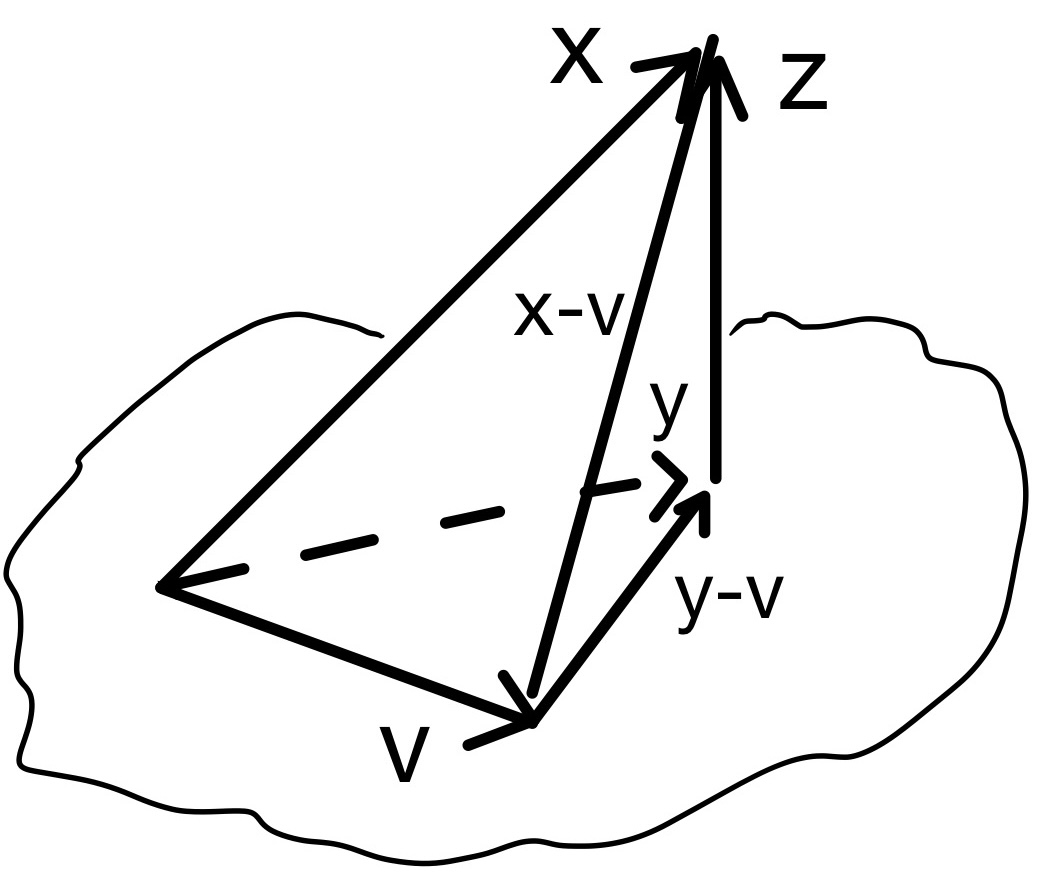
\includegraphics[scale = 0.15]{images/picture1.JPG}    
    \end{center}
    
    \textbf{Свойства операции $\perp$:}\ ($\forall U 
    \subseteq V\longmapsto U^\perp,\ \text{dim }\mathcal{E} 
    <\infty$)

    1. $(U^\perp)^\perp = U$
    
    2. $(U_1 + U_2)^\perp = U_1^\perp \cap U_2^\perp$

    3. $(U_1 \cap U_2)^\perp = U_1^\perp + U_2^\perp$ 
    \begin{proof}
        $\\$ 1. $\forall u \in U,\ \forall v \in U^\perp 
        \Longrightarrow (u,v) = 0 \Longrightarrow u \in 
        (U^\perp)^\perp$\\
        Равенство размерностей: $$\text{dim}U^\perp = n - \text
        {dim}U,\ \text{dim}(U^\perp)^\perp = n - \text{dim}
        U^\perp = \text{dim}U \Longrightarrow U = (U^\perp)
        ^\perp$$
        2. Возьмем $v \in U_1^\perp \cap U_2^\perp$, тогда 
        $\forall w = u_1 + u_2,\ (v,w) = \underbrace{(v,u_1)}_
        {0} + \underbrace{(v,u_2)}_{0} \Longrightarrow$ $$v \in 
        (U_1 + U_2)^\perp \Longrightarrow U_1^\perp \cap 
        U_2^\perp \subseteq (U_1 + U_2)^\perp$$
        Равенство размерностей:
        $$\text{dim}(U_1 + U_2)^\perp = n - \text{dim}(U_1 + 
        U_2) =$$ $$=n - (\text{dim}U_1 + \text{dim}U_2 - 
        \text{dim}(U_1 \cap U_2)) = $$
        $$= n + \text{dim}(U_1 \cap U_2) - \text{dim}U_1
        - \text{dim}U_2 = $$
        $$= (n - \text{dim}U_1) + (n - \text{dim}U_2) + 
        \text{dim}(U_1\cap U_2) - n \Longrightarrow $$
        $$dim(U_1^\perp \cap U_2^\perp) = \text{dim}U_1^\perp
        + \text{dim}U_2^\perp - \text{dim}(U_1^\perp \cap 
        U_2^\perp) = $$
        $$= n- \text{dim}U_1 + n - \text{dim}U_2 - 
        \text{dim}(U_1^\perp + U_2^\perp)$$
        $\text{dim}(U_1^\perp + U_2^\perp) \overset{?}{=}
        n - \text{dim}(U_1 \cap U_2)$\\
        $\text{dim}(U_1^\perp + U_2^\perp) = \text{dim}
        U_1^\perp + \text{dim}U_2^\perp - \text{dim}(U_1^\perp
        \cap U_2^\perp)$\\
        $(U_1 + U_2)\perp \subseteq U_1^\perp \cap U_2^\perp$\\
        Если $v \in (U_1 + U_2)^\perp \Longrightarrow 
        \begin{cases}
            (v, u_1) = 0, \forall u_1 \in U_1\\
            (v, u_2) = 0, \forall u_1 \in U_2
        \end{cases} \Longrightarrow v \in U_1^\perp \cap 
        U_2^\perp$\\
        3. $(U_1 \cap U_2)^\perp = U_1^\perp + U_2^\perp
        \Longleftrightarrow \underbrace{(U_1 \cap U_2)^
        {\perp\perp}}_{U_1 \cap U_2} \overset
        {?}{=} (U_1^\perp + U_2^\perp) = $ (свойство 2) $=$ \\
        $= (U_1^\perp)^\perp \cap (U_2^\perp)^\perp = U_1 \cap 
        U_2$
    \end{proof}
    \begin{center}
        \textbf{Изоморфизм евклидовых пространств.} 
    \end{center}
    $\varphi:\ \mathcal{E} \longmapsto \mathcal{E}'$ --
    изоморфизм евклидовых пространств $\mathcal{E}$ и
    $\mathcal{E}'$, если
    
    1. $\varphi$ -- линейное отображение.
    
    2. $\varphi$ -- биекция.
    
    3. $\forall x_1,x_2 \in \mathcal{E} \Longrightarrow 
    (\varphi(x_1), \varphi(x_2)) = (x_1, x_2)$ 

    \begin{theorem}
        Если $\text{dim }\mathcal{E} = \text{dim }\mathcal{E}
        '$, то $\mathcal{E}$ и $\mathcal{E}'$ изоморфны,
        т.е. существует изоморфизм $\varphi:\ \mathcal{E}
        \longmapsto \mathcal{E}'$   
    \end{theorem}
    \begin{proof}
        Выберем $e_1,...,e_n$ -- О.Н.Б. в $\mathcal{E}$,\
        $e_1',...,e_n'$ -- О.Н.Б. в $\mathcal{E}'$\\
        $\forall x = \sum\limits_{i=1}^{n} x_ie_i$, определим
        $\varphi(x) = \sum\limits_{i=1}^{n} x_ie_i'$
        (в частности, $\varphi(e_i) = e_i'$)\\
        $\varphi$ -- линейный изоморфизм.\\
        $\forall x,y \in \mathcal{E}, (x,y) = \sum\limits_{i=1}^
        {n} x_iy_i$,\ \ $(\varphi(x), \varphi(y)) = 
        (\sum\limits_{i} x_ie_i', \sum\limits_{j}y_je_j') = 
        \sum\limits_{i=1}^{n} x_iy_i = (x,y)$  

    \end{proof}

    \begin{theorem}
        $\\$ 1. Пусть $e, e'$ -- два О.Н.Б. в евклидовом 
        пространстве $\mathcal{E}$,\ $C_{e \to e'} \Longrightarrow C_{e \to e'}^T = C_{e \to e'}^{-1}$
        (ортогональная матрица).\\
        2. Если $e$ -- О.Н.Б., $C$ -- ортогональная матрица,
        то $eC = e'$ -- тоже О.Н.Б.
    \end{theorem}
    \begin{proof}
        $\\$1. Дано: $e'$ -- О.Н.Б. $\Longrightarrow 
        (e_i,e_j) = \delta_{ij}$ (символ Кронекера)
        $$(e_i,e_j) = (C^TC)_{ij} \Longrightarrow C^TC = E$$  
        2. $C_{e \to e'} = (e_1^{'\uparrow}...e_n^
        {'\uparrow})$ в базисе $e$.
        Т.к. базис $e$ ортонормированный, то\\ $(e_i', e_j')=
        e_i'\cdot {e'}_j^{\uparrow}$ -- это $(i,j)$
        элемент произведения:
        $$C^TC = E \Longrightarrow (e_i',e_j') = \delta_{ij}
        \Longrightarrow e' - \text{ О.Н.Б.}$$
    \end{proof}
    \textbf{Понятие объема n-мерного параллелепипеда.}\\
    Параллелепипед $\Pi$ с ребрами $a_1,...,a_n$ в n-мерном
    пространстве $V$.
    $$\Pi = \{\sum\limits_{i=1}^{n} \alpha_ia_i\ |\ 
    0 \leq \alpha_i \leq 1,\ 1 \leq i \leq n\}$$
    Будем считать, что $a_1,...,a_n$ ЛНЗ.\\
    В n-мерном евклидовом пространстве $\mathcal{E}_n$  
    \begin{definition}
        Объемом n-мерного параллелепипеда $V_n$ назывется 
        произведение объема $(n-1)$-мерного основания 
        $\Pi_{\{a_1,...,a_{n-1}\}}$ на высоту $|a_n^\perp|$ 
    \end{definition}

    \underline{Формула:} $|a_n^\perp|^2 = \frac{\text{det}G_{\{a_1,...,a_n\}}}{\text{det}G_{\{a_1,...,a_{n-1}\}}}$
    \begin{proof}
        Ортогонализуем векторы $a_1,...,a_n$ -- получим 
        попарно ортогональные $b_1,...,b_n$ (в частности, $
        b_n \perp b_1,...,b_{n-1},\ \langle b_1,...,b_{n-1}
        \rangle = \langle a_1,...,a_{n-1}\rangle$)
        $$G_{\{b_1,...,b_n\}} = C^TG_{\{a_1,...,a_n\}}C
        \text{, при этом } C = \begin{pmatrix}
            1 & \null & *\\
            \null & \ddots & \null\\
            0 & \null & 1
        \end{pmatrix} \Longrightarrow \text{det}G_{\{b_1,...,b_n\}} = \text{det}G_{\{a_1,...,a_n\}}$$
        $$\frac{\text{det}G_{\{a_1,...,a_n\}}}{\text{det}G_{\{a_1,...,a_{n-1}\}}} = 
        \frac{|b_1|^2...|b_n|^2}{|b_1|^2...|b_{n-1}|^2} = 
        |b_n|^2 = |a_n^\perp|^2$$
    \end{proof}
    \begin{consequense}
        По индукции, $V_n^2 = \text{det}G_{\{a_1,...,a_n\}}$ 
    \end{consequense}
    \begin{consequense}
        $$\rho^2(x,U) = \frac{\text{det}G_{\{a_1,...,a_m,x\}}}{
        G_{\{a_1,...,a_m\}}} (U = \langle a_1,...,a_m\rangle
        \text{ ЛНЗ})$$
    \end{consequense}
    \begin{consequense}
        Если известны координаты векторов $a_1,...,a_n$ в 
        О.Н.Б., то $$V_n = |\text{det}\begin{pmatrix}
            \vec a_1\\\vdots\\\vec a_n
        \end{pmatrix}|$$
    \end{consequense}
    \begin{proof}
        Т.к. базис ортонормированный, то
        $$\begin{pmatrix}
            \vec a_1\\\vdots\\\vec a_1
        \end{pmatrix}(a_1^\uparrow...a_n^\uparrow) = 
        \text{det}G_{\{a_1,...,a_n\}} \Longrightarrow $$
        $$V_n^2 = \text{det}G_{\{a_1,...,a_n\}} = 
        \begin{pmatrix}\text{det}\begin{pmatrix}
            \vec a_1\\\vdots\\\vec a_n
        \end{pmatrix}\end{pmatrix}^2$$
    \end{proof}
    \begin{center}
        \begin{Large}
            \textbf{\S6. Линейный оператор в евклидовом 
            пространстве} 
        \end{Large}
    \end{center}
    Пусть $\mathcal{E}$ -- евклидово пространство, 
    $\varphi:\ \mathcal{E} \longmapsto \mathcal{E}'$
    \begin{definition}
        Оператор $\varphi^*$ -- сопряженный к $\varphi$:\\  
        $\varphi^*:\ \mathcal{E} \longmapsto \mathcal
        {E},\ \forall x,y \in \mathcal{E}:\ (\varphi(x),y) = 
        (x, \varphi^*(y))\ \ (1)$ 
    \end{definition}
    \begin{definition}
        Оператор $\varphi$ -- самосопряженный, если\\
        $\varphi^* = \varphi$, т.е. $\forall x,y \in \mathcal
        {E}:\ (\varphi(x),y) = (x, \varphi(y))$
    \end{definition}
    \begin{definition}
        Оператор $\varphi$ -- ортогональный, если $$\forall
        x,y \in \mathcal{E}:\ (\varphi(x),\varphi(y)) = (x,y)$$
    \end{definition}$\\$
    \textbf{Условия на матрицу $A_\varphi$:}

    1. (1) в координатах:
    $$(A_\varphi X)^TG_eY = X^TG_e(A_{\varphi^*}Y) 
    \Longrightarrow $$ 
    $$X^T(A_\varphi^TG_e)Y = X^T(G_eA_{\varphi^*})Y,\
    \forall X,Y \in F^n \Longrightarrow $$
    $$A_{\varphi}^T G_e = G_e A_{\varphi*} \Longrightarrow $$
    $$A_{\varphi*} = G^{-1}A_\varphi^TG_e$$
    Если $e$ -- О.Н.Б., то $G_e = E$ и $A_{\varphi*} = 
    A_\varphi^T$

    2. $\varphi = \varphi^*$ -- самосопряженный 
    $\Longleftrightarrow (\varphi(x),y) = (x,\varphi(y)),\ 
    \forall x,y \in \mathcal{E} $
    $$(A_\varphi X)^TG_eY = X^TG_eA_\varphi Y,\ \forall
    X,Y \in \mathbb{R}^n $$
    $$X^T(A_\varphi^TG_e)y = X^T(G_eA_\varphi)Y 
    \Longleftrightarrow A_\varphi^TG_e = G_eA_\varphi$$
    В О.Н.Б. $\Longleftrightarrow A_\varphi^T = A_\varphi$
    -- симметричная.

    3. $\varphi$ -- ортогональный $\Longleftrightarrow 
    \forall x,y:\ (\varphi(x),\varphi(y)) = (x,y) \Longleftrightarrow $
    $$(A_\varphi X)^TG_e(A_\varphi Y) = X^T G_e Y$$
    $$X^T(A_\varphi^T G_eA_\varphi)Y \equiv X^TG_eY 
    \Longleftrightarrow A_\varphi^T G_e A_\varphi = G_e$$
    В О.Н.Б.: $A_\varphi^T A_\varphi = E,\ A_\varphi$ --
    ортогональньная.\\$\\$
    \underline{Комментарий к определению $\varphi^*$:}\\
    Пусть $\varphi:\ V \longmapsto W$ -- линейное отображение.\\
    Тогда $\varphi^*:\ \underbrace{W^*}_{f \in } \longmapsto 
    V^*$ определим по правилу:
    $\varphi^*(f)(v) = f(\varphi(v)),\ \forall v \in V$\\
    Это $\varphi^*$ -- линейное отображение, в частности, 
    для $W = V$, то $\varphi^*:\ V^* \longmapsto V^*$ --
    линейный оператор.    

    \begin{subtheorem}
        Если $\mathcal{E}$ -- евклидово пространство, то 
        $\mathcal{E^*} \cong \mathcal{E}$.  
    \end{subtheorem}
    \begin{proof}
        Построение изоморфизма:

        Выберем в $\mathcal{E}$ О.Н.Б. $e,\ \forall v \in \mathcal
        {E} :\ v = \sum\limits_{i=1}^{n} x_ie_i$
        $$\forall f \in \mathcal{E^*},\ f(v) = \sum\limits_{i=
        1}^{n} \underbrace{f(e_i)}_{a_i}x_i = \sum\limits_{i=1}^{n} 
        a_ix_i = (a_1,...,a_n)\begin{pmatrix}
            x_1\\\vdots\\ x_n
        \end{pmatrix} = (a, v)$$
        
        Т.к. базис ортонормированный и $a = \sum\limits_{i=1}^{n} a_ie_i,\ v = \sum\limits_{i=1}^{n} x_ie_i$ 

        Т.е. для функции $f$ найти такой вектор, что $f(v) = (a,v)
        ,\ \forall v \in \mathcal{E}$ 

        $f \longleftrightarrow a$, можно "отождествить" $\mathcal
        {E} \text{ и } \mathcal{E^*} $
    \end{proof}
    $\\$ \textbf{Свойства операции сопряжения:}
    
    1. $(\varphi^*)^* = \varphi$
    
    2. $(\alpha \varphi + \beta \varphi)^* = \alpha \varphi^*
    + \beta \varphi^*$
    
    3. $(\varphi \psi)^* = \psi^* \varphi^*$ 
    \begin{proof}
        Достаточно доказать для матриц в О.Н.Б.

        1. $A_{\varphi^*} = A_\varphi^T \Longrightarrow 
        A_{\varphi^{**}} = (A_{\varphi^*})^T = A_\varphi^{TT} = 
        A_\varphi$ 

        2. Очевидно.

        3. $A_{(\varphi \psi)^*} = A_{\varphi \psi}^T = 
        (A_\varphi A_\psi)^T = 
        A_\psi^T A_\varphi^T = A_{\psi^*}A_{\varphi^*}$ 
    \end{proof}

    \begin{theorem}
        Пусть $\varphi:\ \mathcal{E} \longmapsto \mathcal{E}$
        -- линейный оператор. Тогда:
        
        1.  Если $\varphi(U) \subseteq U$, то $\varphi^*
        (U^\perp) \subseteq U^\perp$

        2. Im$\varphi = (\text{Ker}\varphi^*)^\perp$
        
        3. $\text{Ker}\varphi = (\text{Im}\varphi^*)^\perp$ 
    \end{theorem}
    \begin{proof}
        $\\$1. Пусть $x \in U,\ y \in U^\perp.\ 
        \varphi^*(y) \subseteq U^\perp \Longleftrightarrow$
        \begin{flushright}
            $0 \overset{?}{=} (x, \varphi^*(y)) = (\underbrace
            {\varphi(x)}_{\in U}, y) = 0 \Longrightarrow 
            \varphi^* \in U^\perp$
        \end{flushright}
        2. Возьмем $y \in \text{Im}\varphi \Longrightarrow 
        \exists x \in \mathcal{E}:\ y = \varphi(x)$ 

        Возьмем $z \in \text{Ker}\varphi^*$. Вычислим:
        $$(y,z) = (\varphi(x),z) = (x,\underbrace{\varphi^*(z)}_
        {0}) = 0 \Longrightarrow $$
        $$y \in (\text{Ker}\varphi^*)^\perp \Longrightarrow 
        \text{Im}\varphi \subseteq (\text{Ker}\varphi^*)
        ^\perp$$
        $\text{dimIm}\varphi = \text{rk}A_\varphi,\ 
        \text{dimKer}\varphi^* = n - \text{dimIm}\varphi^* =
        n - \text{rk}A_\varphi$.\\
        Но $\text{rk}A_{\varphi^*} = \text{rk}A_\varphi$
        (в О.Н.Б. $A_{\varphi^*} = A_\varphi^T$) 
        $\Longrightarrow$
        \begin{flushright}
            $\text{dim}(\text{Ker}\varphi^*)^\perp = n - 
            \text{dimKer}\varphi^* = \text{rk}A_\varphi 
            \Longrightarrow \text{размерности равны}$
        \end{flushright}
        3. $\text{Ker} \varphi = (\text{Im} \varphi^*)^\perp
        \Longleftrightarrow (\text{Ker} \varphi)^\perp = 
        \text{Im} \varphi^*$\\
        Заменим $\varphi$ на $\varphi^*$, тогда $\varphi^*$
        на $\varphi^{**}$ в равенстве 2.\\
        Тогда $(\text{Ker} \varphi^*)^\perp = \text{Im}
        \varphi$ в исходных обозначениях это дает 
        $(\text{Ker}\varphi)^\perp = \text{Im} \varphi^*$

    \end{proof}
    \begin{consequense}
        (Теорема Фредгольца)\\
        СЛУ $AX = b\ (*)$ совместна $\Longleftrightarrow \forall
        Y$ -- решения сопряженной однородной системы $A^TY = 0$
        выполняется условие: $Y^Tb = 0$, (т.е $Y \perp b$ )  
    \end{consequense}

    Система (*) совместна означает, что $b \in \text{Im}
    \varphi$, если $A$ -- матрица оператора $\varphi$\\
    По 2, $b \in \text{Im}\varphi \Longleftrightarrow 
    b \in (\text{Ker}\varphi^*)^\perp,$ т.е. $\forall Y:
    A^TY = 0,\ (b,Y) = 0$ 

    \begin{center}
        \begin{Large}
            \textbf{\S7. Самосопряженные операторы.}
        \end{Large}
    \end{center}
    \begin{definition}
        $\varphi:\ \mathcal{E} \longmapsto \mathcal{E}$
        называется самосопряженным, если\\
        $\tab[3.7cm]\forall
        x,y \in \mathcal{E}:\ (\varphi(x), y) = (x,\varphi
        (y))\ \ (1)$
    \end{definition}
    \begin{theorem}
        Пусть $\varphi:\ \mathcal{E} \longmapsto \mathcal{E}$
        -- самосопряженный оператор

        1. Если $U \subseteq \mathcal{E}$ -- 
        $\varphi$-инвариантное подпространство, то $U^\perp$ 
        также \\$\tab[1.2cm]\varphi$-инвариантно (это доказано для 
        $\varphi^*$ )

        2. Все характеристические корни $\varphi$ 
        вещественные.  

        3. В $\mathcal{E}$ существует О.Н.Б. из собственных
        векторов оператора $\varphi$
        \\ $\tab[1cm]$  (в нем $A_\varphi$ диагональна).  
    \end{theorem}
    \begin{proof}
        $\\$2. Пусть $\lambda_1$ -- характеристический корень
        для $\chi_\varphi(\lambda)$\\
        Если $\lambda_1 \in \mathbb{R}$ -- это собственное 
        значение, и доказывать нечего. (C) Чубаров\\
        Если $\lambda_1 = \alpha + i \beta$, то существует
        двумерное инвариантное подпространство $U = \langle
        X,Y \rangle,\ X,Y \in \mathbb{R}^n$.\\
        $(x,y)|_U$ делает его евклидовым пространством.\\
        $(x,y \in U),$ соотвественно, $\varphi|_U$ будет
        самосопряженным оператором на $U \Longrightarrow $\\
        в О.Н.Б. $e_1',e_2',\ A_{\varphi|_U} = A, \text{ т.е. } 
        A = \begin{pmatrix}
            a_{11} & a_{12}\\
            a_{12} & a_{22}
        \end{pmatrix}$    
        $$\begin{vmatrix}
            a_{11} - \lambda & a_{12}\\
            a_{12} & a_{22} - \lambda
        \end{vmatrix} = \lambda^2 - (a_{11} + a_{22})\lambda
        + a_{11}a_{22} - a_{12}^2$$
        $$D = (a_{11} + a_{22})^2 - 4(a_{11}a_{22} - a_{12}^2)
        = (a_{11} - a_{22})^2 + 4a_{12}^2 \geq 0 
        \Longrightarrow \lambda \in \mathbb{R} $$
        3. Индукция по $\text{dim}\mathcal{E} = n$:

        dim$\mathcal{E} = 1 \Longrightarrow \varphi(x) = 
        \lambda x,\ \forall x \in \mathcal{E} $ -- верно.

        Для dim$\mathcal{E} = n > 1$ предположение
        индукции: в $(n-1)$-мерном евклидовом пространстве
        самосопряженный оператор имеет О.Н.Б. из 
        собственных векторов.

        Фикс. одно собственное значение $\lambda_1 \in 
        \mathbb{R}$, обозн. $U = \langle e_1\rangle,$ если\\
        $\varphi(e_1) = \lambda_1 e_1,\ |e_1| = 1$

        Тогда $U^\perp $ имеет размерность $(n-1)$ является
        евклидовым относительно $(x,y)|_{U^\perp}$ и 
        $\varphi|_{U^\perp}$ -- самосопряженный 
        $\Longrightarrow $  в $U^\perp\ \exists$ О.Н.Б.
        $e_2,...,e_n:\ \varphi(e_i) = \lambda_ie_i$

        Тогда $e_1,...,e_n$ -- нужный О.Н.Б. 
    \end{proof}
    \underline{Задача:} Пусть $\varphi$ -- самосопряженное
    оператор в $\mathcal{E},\ \varphi^2 = \varphi$ 
    (идемпотентный оператор). Тогда либо $\varphi = \mathcal{E} 
    $ или $0$, либо $\varphi$ -- ортогональнное проектирование
    $\mathcal{E} $ на некоторое подмножество. 

    \begin{center}
        \begin{Large}
            \textbf{\S8. Ортогональные операторы.}
        \end{Large}
    \end{center}
    \begin{definition}
        Линейный оператор $\varphi:\ \mathcal{E} \longmapsto 
        \mathcal{E} $ назывется ортогональным, $\tab[3.5cm]$ 
        если $
        \forall x,y \in \mathcal{E}:\ (\varphi(x),\varphi(y)) 
        = (x,y)$
    \end{definition}
    Заметим, что $|\varphi(x)| = |x|,\ \forall x \in \mathcal{E}
    \Longrightarrow \varphi$ -- невырожденный.

    \begin{theorem}
        $\varphi:\ \mathcal{E} \longmapsto \mathcal{E}$ --
        ортогональный оператор.

        1. Собственные векторы, отвечающие различным 
        собственным значениям\\ $\tab[1cm]$ ортогональны. 

        2. Все характеристические корни ортогональльной матрицы 
        $|\lambda| = 1$,\\ $\tab[1cm]$ 
        вещественные только $\pm 1$.

        3. Если $\varphi(U) \subseteq U$, то 
        $\varphi(U^\perp) \subseteq U^\perp$  

    \end{theorem} 
    \begin{proof}
        $\\$3. Пусть $x \in U, y \in U^\perp$,\ 
        $0 = (x,y) = (\varphi(x), \varphi(y))$\\
        Т.к. $\varphi$ невырожденно, т.е. обратимо, то
        $\forall x \in U\ \exists z \in U\ (z = \varphi^{-1}(x))
        $  
        $$(x,y) = (\varphi^{-1}(x), y) = (\varphi(\varphi^{-1}
        (x)), \varphi(y)) = (x, \varphi(y)) \Longrightarrow 
        \varphi(y) \in U^\perp$$
        $\varphi^{-1}$ тоже ортогонален.\\
        1. Пусть $\varphi(x) = \lambda_1 x,\ x \neq 0,\ 
        \varphi(y) = \lambda_2 y,\ y \neq 0,\ \lambda_1 \neq 
        \lambda_2$:
        $$(\varphi(x), \varphi(y)) = \lambda_1\lambda_2
        (x,y) = (x,y)$$
        $$(x,y)(1 - \underbrace{\lambda_1\lambda_2}_{-1}) = 0 \Longrightarrow 
        2(x,y) = 0 \Longrightarrow (x,y) = 0$$ 
        2. Если $\lambda$ -- собственное значение, то $\lambda
        \in \{1,-1\},\ \varphi(x) = \lambda x,\ x \neq 0:$
        $$(\varphi(x), \varphi(x)) = \lambda^2(x,x) = 
        \underbrace{(x,x)}_{\neq 0} \Longrightarrow 
        \lambda^2 = 1,\ \lambda = \pm 1$$
        Если $\lambda_1 = \alpha + i \beta,\ (\beta \neq 0)$
        -- корень матрицы $A_\varphi$, то рассмотрим оператор
        $\varphi^\mathbb{C}:\ \mathbb{C}^n \longmapsto 
        \mathbb{C}^n,\ (\text{dim}V = n)$
        $$\varphi^\mathbb{C} (z) = \lambda_1z,\ z = 
        \begin{pmatrix}
            x_1\\\vdots\\x_n
        \end{pmatrix}$$
        $$((1,i),(1,i)) \overset{?!}{=} 1\cdot 1 + 
        i \cdot i$$
        Введем в $\mathbb{C}^n$ скалярное произведение 
        векторов $X, Y:$
        $$(X,Y):= \sum\limits_{i=1}^{n} x_i \overline{y_i}
        \Longrightarrow (X,X) = \sum\limits_{i=1}^{n} |x_i|^2$$ 
        При этом, $(Y,X) = \overline{(X, Y)}$, в частности,
        $\forall \lambda \in \mathbb{C},\ (X, \lambda Y) = 
        \overline{\lambda}(X,Y)$\\
        Пусть $x \in \mathbb{C}^n$ -- собственный для 
        $\varphi^\mathbb{C}$, т.е. $A_\varphi X = \lambda_1X$,
        вычислим $$(\varphi^\mathbb{C}(x), \varphi^\mathbb{C} 
        (x)) = (x,x)$$
        $$(\lambda_1X, \lambda_1X) = \lambda_1\overline
        {\lambda_1}(X,X) \Longrightarrow |\lambda_1|^2 = 1,\
        |\lambda| = \pm 1$$

    \end{proof}
    \begin{definition}
        Матрица называется канонической, если
        $$A = \begin{pmatrix}
            \Phi_1 & \null & \null & \null & \null & \null & \null & \null & \null\\
            \null & \ddots & \null  & \null & \null & \null & \null & \null & \null\\
            \null & \null & \Phi_s & \null & \null & \null & \null & \null & \null\\
            \null & \null & \null & 1 & \null & \null & \null & \null & \null\\
            \null & \null & \null & \null & \ddots & \null & \null & \null & \null\\
            \null & \null & \null & \null & \null & 1 & \null & \null & \null\\
        \end{pmatrix}$$ 
    \end{definition}










    \begin{theorem}
        Для любого ортогонального оператора в $\mathcal{E}_n$
        существует ортонормированный базис, в котором матрица 
        $A_\varphi$ имеет канонический вид, при этом числа 
        $p,q,s$ и углы $\alpha_k\ (k=1,...,s)$ для $\varphi$
        опеределяется единственным образом, с точностью до
        порядка следования клеток.
    \end{theorem}
    \begin{proof}
        Допустим, что $\varphi$ имеет хотя бы одно 
        вещественное собственное значение. Рассмотрим $U = 
        \mathcal{E}_1 \oplus \mathcal{E}_{-1}$ (прямая сумма
        собственных подпространств). Обозначим за $p := 
        \text{dim}\mathcal{E}_1,\ q := \text{dim}U_{-1}
        \Longrightarrow \text{dim}U  = p + q$.\\
        $U$ -- инвариантное подпространство, тогда 
        $\mathcal{E} = U^\perp \oplus U,\ U^\perp $
        также инвариантно, и $\varphi|_{U^\perp}$
        не имеет вещественных собственных значений.
        Возьмем одно из них $\lambda_1 = \cos \alpha_1 + 
        i\sin \alpha_1 \sim L_1$.
        $$A_{\varphi|_{L_1}} = \begin{pmatrix}
            \cos \alpha_1 & - \sin \alpha_1\\
            \sin \alpha_1 & \cos \alpha_1
        \end{pmatrix}$$
        Индукция по размерности $s$ (если $s\neq 0$), 
        $\text{dim}U^\perp = 2s$.\\
        Рассмотрим подпространство: $L_1^\perp$ в пространстве
        $U^\perp$, его размерность равна $2s - 2$.\\
        По предположению индукции, в $L_1^\perp$ в $U^\perp$
        существует О.Н.Б., в котором матрица ограничения
        оператора $\varphi$ имеет вид
        $$\begin{pmatrix}
            \Phi_2 & \null & 0\\
            \null & \ddots & \null\\
            0 & \null & \Phi_n
        \end{pmatrix}$$
    \end{proof}
    \textbf{Пример:} Пусть $A^T = A^{-1}$ 3-го порядка.
    Хотим найти матрицу $$A \overset{?}{\sim} A' = 
    \begin{pmatrix}
        \cos \alpha & -\sin \alpha & 0\\
        \sin \alpha & \cos \alpha & 0\\
        0 & 0 & \lambda_1
    \end{pmatrix},\ \lambda_1 = \pm 1$$
    $$|A'| = \begin{vmatrix}
        \cos \alpha & -\sin \alpha\\
        \sin \alpha & \cos \alpha
    \end{vmatrix} \lambda_1 = \lambda_1 = \pm 1$$
    Зная, что можно вычислить собственный вектор 
    $\Longrightarrow $ он дает ось поворота (м.б. с симметрией,
    если $\lambda_1 = -1$)
    $$\text{tr}A = \text{tr}A' = 2\cos \alpha + \lambda_1
    \Longrightarrow \cos \alpha = \frac{\text{tr}A - \lambda_1}
    {2}$$
    Можно выбрать правый О.Н.Б. $e_1,e_2$ в плоскости, $\perp
    e_3,\ \varphi(e_3) = \lambda_1e_3,\ |e_3| = 1.$\\
    \underline{Общий случай:} $\varphi:\mathcal{E} 
    \longmapsto \mathcal{E}.$
    \begin{lemma}
        Если $\varphi$ невырожденная, то все собственные 
        значения оператора $\varphi^*\cdot \varphi$
        положительны. 
    \end{lemma}
    \begin{theorem}
        Любой невырожденный оператор $\varphi$ может быть
        представлен в виде произведения (причем единственным 
        образом) $\varphi = \theta 
        \cdot\psi$, где $\theta$ -- ортогональный оператор, а 
        $\psi$ -- самосопряженный со всеми положительными 
        собственными значениями $\lambda > 0$. 
    \end{theorem}
    \begin{proof}
        Пусть $\mu$ -- собственное значение оператора 
        $\varphi^*\cdot \varphi,\ (\varphi^*\cdot \varphi)
        (x) = \mu x,\ x \neq 0$
        Вычислим: $((\varphi^*\cdot \varphi)(x), x) = 
        \mu(x,x)$
        $$(\underbrace{\varphi(x)}_{\neq 0}, \varphi(x)) > 0 
        \Longrightarrow 
        \mu = \frac{(\varphi(x), \varphi(x))}{(x,x)} > 0$$
        Матричная формулировка: любую невырожденную 
        вещественную матрицу $A$ можно представить, причем
        единственным образом, в виде $A = BC$, где 
        $B^T = B^{-1},\ C^T = C$, с положительными
        собственными значениями.\\
        Такое разложение называется полярным разложением
        оператора (матрицы).\\
        Можно выбрать О.Н.Б. $e_1,...,e_n$ в $\mathcal{E}$,
        тогда $A = A_\varphi,\ B = B_\theta,\ C = C_\psi.$\\
        Доказательство матричного варианта:\\
        Пусть задача решена: $$A = BC \Longrightarrow A^T =
        C^TB^T = CB^{-1} \Longrightarrow A^TA = 
        CB^{-1}BC = C^2$$
        Т.к. матрица $A^TA = C^2$ -- симметричная, она задает
        самосопряженный линейный оператор, т.е. существует
        О.Н.Б. $e_1',...,e_n'$, в котором $$(A^TA)' = 
        \begin{pmatrix}
            \mu_1 & \null & 0\\
            \null & \ddots & \null\\
            0 & \null & \mu_n    
        \end{pmatrix} \text{ все } \mu_i > 0, \text{ по лемме}.
        $$
        Хотим найти матрицу $C'$, чтобы 
        $$(C')^2 = \begin{pmatrix}
            \mu_1 & \null & 0\\
            \null & \ddots & \null\\
            0 & \null & \mu_n    
        \end{pmatrix} \Longrightarrow C' = \begin{pmatrix}
            \pm\sqrt{\mu_1} & \null & 0\\
            \null & \ddots & \null\\
            0 & \null & \pm\sqrt{\mu_n}
        \end{pmatrix}$$ 
        С учетом требования положительности
        $$C' = \begin{pmatrix}
            \lambda_1 & \null & 0\\
            \null & \ddots & \null\\
            0 & \null & \lambda_n    
        \end{pmatrix},\ \lambda_i = \sqrt{\mu_i} > 0 -
        \text{ единственная такая матрица.}$$
        Пусть $T$ -- (ортогональная) матрица перехода от
        базиса $e$ к базису $e'$, тогда
        $$T^{-1}(A^TA)T = \begin{pmatrix}
            \mu_1 & \null & 0\\
            \null & \ddots & \null\\
            0 & \null & \mu_n    
        \end{pmatrix} \Longrightarrow C = TC'T^{-1} = 
        T\begin{pmatrix}
            \lambda_1 & \null & 0\\
            \null & \ddots & \null\\
            0 & \null & \lambda_n    
        \end{pmatrix}T \Longrightarrow $$
        $$B = AC^{-1} - \text{ эта матрица оргональная}$$
        $$B^T = (C^{-1})TA^T = C^{-1}A^T \Longrightarrow B^TB = 
        (C^{-1}A^T)(AC^{-1}) = C^{-1}(\underbrace{A^TA}_{C^T})C^
        {-1} = E$$

    \end{proof}
    \begin{remark}
        Можно также представить $A$ в виде $A = C'B'$. Вопрос:
        можно ли утверждать, что $B' = B$ или $C' = C$?  
    \end{remark}
    Рассмотрим разложение $A = BC$, где $C = T\begin{pmatrix}
        \lambda_1 & \null & 0\\
        \null & \ddots & \null\\
        0 & \null & \lambda_n
    \end{pmatrix}T^{-1}$
    $$A = (BT)diag(\underset{\text{все } > 0}{\lambda_1,...,
    \lambda_n})T^{-1} = D\cdot diag(\lambda_1,...,\lambda_n)
    F,$$ где $F, D$ -- ортогональное сингулярное разложение. 
    \begin{center}
        \begin{Large}
            \textbf{\S9. Квадратичные формы на евклидовом 
            пространстве.}
        \end{Large}
    \end{center}

    Пусть $k(x) = f(x,x)$ -- квадратичная функция на евклидовом
    пространстве. 
    $f(x,y)$ -- симметрическая билинейная форма, которая ее 
    порождает.\\
    Обозначим $F$ -- матрицу этой формы в некотором 
    ортонормированном базисе.  
    Если ввести другой О.Н.Б. $e' = eC,\ C = C_{e \to e'}$
    -- ортогональная матрица.\\
    Тогда $F' = C^TFC = C^{-1}FC.$ Поэтому можно рассмотреть
    $F$ как матрицу линейного оператора $\varphi$ в базисе $e$,
    $\varphi$ -- самосопряженный.\\
    По теореме, в $\mathcal{E}$ существует О.Н.Б. $e'$, 
    в котором матрица этого оператора диагональная: 
    $diag(\lambda_1,...,\lambda_n)$.
    $$F_{e'} = C^{-1}FC = C^TFC$$
    Т.е. в базисе $e'$, если сделать замену $X = CY$
    форма $k$ приобретает вид: 
    $$k(y) = \lambda_1y_1^2 +...+ \lambda_ny_n^2$$
    Причем $\lambda_1,...,\lambda_n$ -- собственные 
    значения матрицы $F$.\\
    Базисные векторы $e_1',...,e_n'$ называют главными осями
    для квадратичной формы $k(x)$.  
    %лекция 15.04.
    \begin{definition}
        Линейный оператор $\varphi:\ \mathcal{E} \longmapsto
        \mathcal{E} $ называется присоединенным к билинейной
        функции $f(x,y)$, если: $$\forall x,y \in \mathcal{E}
        f(x,y) = (x,\varphi(y))\ \ (1)$$
    \end{definition}    
    \begin{subtheorem}
        1. Для любой билинейной функции $f(x,y)$ существует
        единственный присоединенный оператор, удовлетворяющий
        тождеству (1)

        2. Если $f(x,y) \equiv f(y,x)$, то $\varphi$ -- 
        самосопряженный. 
    \end{subtheorem}
    \begin{proof}
        Пусть $e$ -- некоторый базис в $\mathcal{E},\ 
        x = eX,\ y = eY \Longrightarrow$
        $$f(x,y) = X^TFY \equiv X^T(G_eA_\varphi)Y
        \Longleftrightarrow F = G_eA_\varphi,\ A_\varphi
        = G_e^{-1}F\ \ (2)$$
        Проверка самосопряженности для симметричности $f(x,y)$:
        $$\forall x,y \in \mathcal{E}\ (\varphi(x),y) = 
        (y,\varphi(x)) = f(y,x) = f(x,y) = (x,\varphi(y))$$         
    \end{proof}
    \begin{theorem}
        (О паре квадратичных форм).\\
        Если $f(x),\ g(x)$ -- квадратичные формы на 
        $\mathcal{E}$ и $g > 0$ , то в $\mathcal{E}$ существует такой 
        базис $e'$, что в новых координатах $$f = \lambda_1y_1^2
        +...+\lambda_ny_n^2,\ g = y_1^2+...+y_n^2$$
    \end{theorem}
    \begin{proof}$\\$
        Обозначим $f(x,y)$ и $g(x,y)$ -- симметричные 
        билинейные функции:\\ $f(x,x) = f(x),\ g(x,x) = g(x),\ 
        F$ и $G$ их матрицы в некотором базисе $e$.\\
        Можно ввести в пространстве $\mathcal{E}$ скалярное 
        произведение $(x,y) := g(x,y)$\\
        Пусть $\varphi:\ \mathcal{E} \longmapsto \mathcal{E}$
        -- линейный оператор, присоединенный к билинейной
        форме $f(x,y)$, т.е. $\forall x,y:\ f(x,y) = g(x,
        \varphi(y))$\\
        Т.к. оператор $\varphi$ самосопряженный, то по 
        основной теореме о самосопряженных операторах
        в пространстве $\mathcal{E}$ существует базис 
        из собственных векторов для $\varphi$ 
        ортонормированный относительно скалярного произведения
        $g(x,y).$\\
        Пусть $e'$ -- этот базис, $C$ -- матрица перехода от
        $e$ к $e'$
        $$X = CY \Longrightarrow g(y) = y_1^2 +...+ y_n^2
        = (y,y)$$
        $$F' = C^TFC;\ \ F = GA_\varphi;\ \ A_\varphi' = 
        \begin{pmatrix}
            \lambda_1 & \null & 0\\
            \null & \ddots & \null\\
            0 & \null & \lambda_n
        \end{pmatrix}$$
        $$G' = C^TGC = E \Longrightarrow GC = (C^T)^{-1}$$
        Тогда $$C^{-1}A_\varphi C = C^{-1}G^{-1}FC = C^TFC = 
        \begin{pmatrix}
            \lambda_1 & \null & 0\\
            \null & \ddots & \null\\
            0 & \null & \lambda_n
        \end{pmatrix} \Longrightarrow $$
        $$f(y) = \lambda_1y_1^2+...+ \lambda_ny_n^2$$
    \end{proof}
    \begin{remark}
        $\lambda_1,...,\lambda_n$ -- собственные значения 
        матрицы $A_\varphi = G^{-1}F$, т.е. они являются 
        корнями уравнения $|A_\varphi - \lambda E| = 0$,
        т.е. $$|G^{-1}F - \lambda E| = 0 \Longleftrightarrow 
        |GG^{-1}F - \lambda G| = |F - \lambda G| = 0$$
        ($\lambda$-уравнение пары матриц $F,\ G$)\\
        Для каждого корня $\lambda_i$ надо решить систему 
        уравнений $$(G^{-1}F - \lambda_iE)X = 0
        \Longleftrightarrow (F - \lambda_i G)X = 0$$
        \begin{flushright}
            $\square$
        \end{flushright}
    \end{remark}
    \textbf{Пример применения:}

    Найти наибольшие и наименьшие значения квадратичной 
    формы $f(x)$ в $\mathbb{R}^n$ при условии, что $g(x) = 
    1$, где $g(x)$ -- положительно опеределенная квадратичная
    форма.\\
    \underline{Решение:} Можно найти такую замену переменных
    $X = CY$, что $$f(x) = \lambda_1y_1^2 +...+ 
    \lambda_ny_n^2\tab[1cm] g(y) = y_1^2+...+ y_n^2 = 1
    \text{ -- единичная сфера в } \mathbb{R}^n $$
    Ответ: $f_{\max} = \max\ \lambda_i,\ \ f_{\min} = 
    \min\ \lambda_i$ (додумать)
    \begin{center}
        \begin{Large}
            \textbf{\S10. Полуторалинейные функции (формы.)}
        \end{Large}
    \end{center}
    Пусть $V$ -- векторное пространство над полем $\mathbb{C}$.
    \begin{definition}
        Функция $\beta:\ V\times V \longmapsto \mathbb{C}$
        называется полуторалинейной, если 

        1. $\forall x_1, x_2, y \in V$ вып. $\beta(x_1 + x_2,y)
        = \beta(x_1,y) + b(x_2,y)$ и

        $\tab[0.5cm]\forall \lambda \in \mathbb{C} $ вып. $\beta(\lambda
        x, y) = \lambda \beta(x,y)$. Линейность по 1 аргументу.

        2. $\beta(x,y_1 + y_2) = \beta(x,y_1) + \beta(x, y_2)$ и

        $\tab[0.5cm]\beta(x,\lambda y) = \overline{\lambda}\beta
        (x,y)$ 
    \end{definition}
    
    В координатах: $$\beta(x,y) = \beta(\sum\limits_{i=1}^{n}
    x_ie_i, \sum\limits_{j=1}^{n} y_je_j) = \sum\limits_{i,j=1}^
    {n} \beta(x_ie_i, y_je_j) = \sum\limits_{i,j=1}^{n} 
    \beta(e_i,e_j)x_i\overline{y_j}$$
    $$B_e = (\beta(e_i,e_j)) \text{ -- матрица формы }
    \beta \text{ в базисе } e.$$
    $$\beta(x,y) = X^TB_e\overline{Y}\tab[1cm] (1)$$

    Квадратичная форма $q:= \beta(x,x) \not\equiv 0$.
    $$q(x) = \sum\limits_{i,j=1}^{n} b_{ij}x_i\overline{x_j}$$
    Если $\beta_{ij} = 0,$ при $i \neq j$, остается $b_{ij}
    = \beta(e_i,e_j)$
    $$q(x) = \sum\limits_{i=1}^{n} b_{ii} x_i\overline(x_i)
    = \sum\limits_{i=1}^{n} b_{ii}|x_i|^2$$

    Эрмитова форма (или эрмитово симметричная)\\
    $\forall x,y \in V$ вып. $\beta(y,x) = \overline{\beta
    (x,y)}$\\
    Тогда $\beta(x,x) = \overline{\beta(x,x)}$, т.е. 
    $\forall x\in V$ вып. $q(x) = \beta(x,x) \in \mathbb{R}$\\
    \underline{Задача.} Для термитово квадратичной формы 
    $q(x)$ существует единственная форма $\beta(x,y):
    \beta(x,x) = q(x)\ \forall x \in V$. 
    \begin{remark}
        $\beta(x,y)$ эрмитова $\Longleftrightarrow B_e^T = 
        \overline{B_e} \Longleftrightarrow \overline{B_e^T}
        = B_e$   
    \end{remark}
    \begin{theorem}
        (О приведении эрмитово квадратичной формы к
        каноническому\\ (нормальному) виду).\\
        Для любой эрмитовой формы (полуторалинейной)
        существует базис, в котором $\beta(x,y) = \sum\limits_
        {i=1}^{n} b_{ii} x_i\overline{y_i}$. Точнее,
        $$\beta(x,y) = x_1\overline{y_1} + ... + 
        x_p\overline{y_p} - x_{p+1}\overline{y}_{p+1} -...-
        x_{p+q}\overline{y}_{p+q},$$ где $p+q = \text{rk}B$.
        Соотвественно $q(x) = |x_1|^2 +...+ |x_p|^2 - |x_{p+1}|
        ^2 -...- |x_{p+q}|^2$ ($q$ и $p$ единствененны).
    \end{theorem}
    \begin{definition}
        Эрмитова квадратичная форма положительно опеределенная,
        если $q(x) > 0\ \forall x \neq 0$. Отрицательно 
        опеределенная, если $q(x) < 0\ \forall x\neq 0$.\\
        (Критерий Сильвестра сохранятеся без изменений).
    \end{definition}
    \begin{center}
        \begin{Large}
            \textbf{\S11. Унитарные (эрмитовы) пространства.}
        \end{Large}
    \end{center}
    \begin{definition}
        Векторное пространство $\mathcal{H}$ над полем $\mathbb
        {C}$ называется унитарным, если на этом $\mathcal{H}$
        задано скалярное произведение $(x,y)$ 
        полуторалинейная форма (полуторалинейная по 2 
        аргументу), эрмитова: $(y,x) = \overline{(x,y)}$ и 
        $(x,x) > 0,\ \forall x \neq 0$. 
    \end{definition}
    \begin{definition}
        $|x| = \sqrt{(x,x)}$ -- длина вектора. \\Неравенство 
        КБШ: $\forall x,y \in \mathcal{H}:\ |(x,y)| \leq |x|
        \cdot |y|$\\
        $\cos \varphi(x,y) = \frac{(x,y)}{|x|\cdot |y|} \in 
        \mathbb{C}$\\
        $(x,y) = 0 \Longleftrightarrow x \perp y$
    \end{definition}
    \begin{theorem}
        (Ортогонализация).\\ В $\mathcal{H}$ существует 
        ортогональльный (и ортонормированный) базис.
    \end{theorem}
    \begin{center}
        \textbf{Изменение матрицы полуторалинейной формы.}
    \end{center}
    При замене базиса: $B' = C^TB\overline{C}$\\
    $\beta(x,y) = X^TB\overline{Y}$ -- в исходном базисе.
    $$X = CX',\ Y = CY' \Longrightarrow$$ $$\beta(x,y) = 
    (CX')^TB\overline{(CY')} = (X')^T(C^TB\overline{C})
    \overline{Y'} \equiv (X')^TB'\overline{Y'} \Longrightarrow $$ $$B' = C^TB\overline{C}$$
    \begin{theorem}
        Если $e$ и $e'$ два О.Н.Б., то матрица перехода 
        $C_{e \to e'}$ унитарно, т.е. если ее подвергнуть 
        эрмитову сопряжению, то она превратится в обратную: $C_{e \to e'}^* = \overline{C}_{e 
        \to e'}^T = C_{e \to e'}^{-1}$    
    \end{theorem}
    \begin{proof}
        По определению матрица перехода, $C = (e_1'^\uparrow
        ,...,e_n'^\uparrow) \Longrightarrow$
        $$C^T = \begin{pmatrix}
            e_1'\\\vdots\\ e_n'
        \end{pmatrix} \Longrightarrow C^T\overline{C}_{ij} =
        e_i'e_j'^\uparrow$$
        Т.к. базис $e$  О.Н., то
        $e_i'e_j'^\uparrow = (e_i'e_j')$\\
        Т.к. базис $e'$ О.Н., то $(e_i'e_j') = \delta_{ij} 
        \Longrightarrow $
        $$C^T\overline{C} = E \Longrightarrow \overline{C^T
        \overline{C}} = \overline{E} = E \Longrightarrow 
        \overline{C}^TC = E \Longrightarrow  \overline{C}^T = 
        C^{-1}$$  
    \end{proof}
    Процесс ортогонализации:

    Если попарно ортогональные векторы $e_1',...,e_{k-1}'\ 
    (k \geq 2)$ уже построены, то
    $$e_k' = e_k - \sum\limits_{i=1}^{k-1} \lambda_ie_i\ |
    \cdot e_j' \text{ справа } (1 \leq j \leq k - 1) 
    \Longrightarrow $$ 
    $$(e_k',e_j') = (e_k,e_j') - \sum\limits_{i=1}^{k-1} 
    (\lambda_ie_i',e_j') = (e_k', e_j') - \lambda_j(e_j',e_j')
    \Longrightarrow $$
    $$\text{pr}_{\langle e_1',...,e_{k-1}'\rangle}(e_k) =
    \sum\limits_{i=1}^{k-1} \frac{(e_k,e_i')}{(e_i',e_i')}
    e_i' $$
    $U^\perp = \{u \in \mathcal{H}| (x,y) = 0,\ \forall
    x \in U\}$\\
    $U \subset \mathcal{H},\ \ \mathcal{H} = U \oplus U^\perp $ 
    \begin{center}
        \begin{Large}
            \textbf{\S12. Линейный операторы в унитарном пространстве.}
        \end{Large}
    \end{center}
    Пусть $\varphi:\mathcal{H} \longmapsto \mathcal{H}$ --
    линейный оператор (над $\mathbb{C}$).\\
    1. Сопряженный оператор: $\forall x,y \in \mathcal{H}:
    (\varphi(x), y) = (x, \varphi^*(y))$
    
    Матрица $A_{\varphi^*}$ (в О.Н.Б.):
    $$(\varphi(x), y) = (A_{\varphi}X)^T\overline{Y} = 
    X^TA_\varphi\overline{Y}^T = X^T\overline{(A_{\varphi^*}
    Y)} = X^T\overline{A}_{\varphi^*}\overline{Y}$$
    $$\forall X,Y \in \mathbb{C} \Longrightarrow 
    \overline{A}_{\varphi^*} = A_\varphi^T \Longleftrightarrow 
    A_{\varphi^*} = \overline{A}_\varphi^T = A_\varphi^*$$
    2. Самосопряженный: $\varphi^* = \varphi 
    \Longleftrightarrow A_\varphi = A_\varphi^*$ (в любом 
    О.Н.Б.), т.е. $A_\varphi$ эрмитова.\\
    3.Унитарный:
    $$\forall x,y \in \mathcal{H}:\ (\varphi(x), \varphi(y))
    = (x,y) \Longleftrightarrow \text{в любом О.Н.Б.}$$
    $$(A_\varphi X)^T \overline{(A_\varphi Y)} = X^T
    (A_\varphi^T\overline{A}_\varphi)\overline{Y} = X^T
    \overline{Y},\ \forall X,Y \in \mathbb{C} 
    \Longleftrightarrow $$ 
    $$A_\varphi^T\overline{A}_\varphi = E \Longleftrightarrow 
    A_\varphi^* A_\varphi = E,\text{ т.е. } A_\varphi
    \text{ -- унитарна.}$$
    \begin{consequense}
        Если $\varphi$ -- унитарный оператор, то $|\text{det}
        A_\varphi| = 1$
    \end{consequense}
    \begin{proof}
    $$|E| = |\overline{A}_\varphi^T A_\varphi| = |\overline
    {A}_\varphi||A_\varphi| = \overline{|A_\varphi|} |A_\varphi|
    = |\text{det}A_\varphi|^2 = 1 \Longleftrightarrow |\text
    {det}A_\varphi| = 1$$
    \end{proof}
    \textbf{Свойства операторов:}
    \begin{theorem}
        Если $\varphi:\mathcal{H} \longmapsto \mathcal{H}$ --
        самосопряженный оператор, то\\
        1. Собственные значения 
        $\lambda \in \mathbb{R}$\\
        2. Собственные векторы, овечающие различным собственным
        значениям перпендикулярны.\\
        3. Если $U \subset \mathcal{H}$ инвариантно 
        относительно $\varphi$, то $U^\perp$ инвариантно.\\
        4. В $\mathcal{H}$ существует О.Н.Б. из собственных
        векторов для $\varphi$, и в нем 
        $$A_\varphi = \begin{pmatrix}
            \lambda_1 & \null & 0\\
            \null & \ddots & \null\\
            0 & \null & \lambda_n
        \end{pmatrix},\ \forall i = 1,...,n,\ \lambda_i \in 
        \mathbb{R}$$  
    \end{theorem}
    \begin{proof}
        $\\$1. Если $x \in \mathcal{H},\ x \neq 0:\ 
        \varphi(x) = \lambda x,$ то\\
        $\begin{cases}
        (\varphi(x), x) = (\lambda x, x) = \lambda(x,x)\\
        (x,\varphi(x)) = (x,\lambda x) = \overline{\lambda}
        (x,x)
        \end{cases} \Longrightarrow \overline{\lambda} = 
        \lambda \in \mathbb{R}$\\ 
    2. Пусть $\varphi(x) = \lambda x,\ x \neq 0,\ \varphi(y) =
    \mu y,\ y \neq 0,\ \lambda \neq \mu \overset{?}
    {\Longrightarrow} (x,y) = 0$\\
    Вычислим 
    $\begin{cases}
        (\varphi(x), y) = \lambda (x,y)\\
        (x, \varphi(y)) = (x, \mu y) = \overline{\mu} (x,y) = 
        \mu(x,y)
    \end{cases} \Longrightarrow$
    \begin{flushright}
        $(x,y)\underbrace{(\lambda - \mu)}_
        {\neq 0} = 0 \Longrightarrow (x,y) = 0$    
    \end{flushright}
    3. Пусть $x \in U,\ y \in U^\perp.$ Надо доказать, что 
    $(x,\varphi(y)) = 0$ \\
    По опр. $(x,\varphi(y)) = (\underset{\in U}{\varphi(x)}, y)
    = 0$\\
    4. Пусть $\lambda_1,...,\lambda_s$ -- все различные 
    собственные значения для $\varphi$.
    Возьмем, $U = \mathcal{H}_{\lambda_1} $ -- собственное 
    подпространство -- оно инвариантно. $\Longrightarrow 
    U^\perp$ также инвариантно, $\mathcal{H} = U \oplus 
    U^\perp$, собственные значения $\varphi|_{U^\perp}$
    -- это $\lambda_2,...,\lambda_s$.\\
    Индукция по $\text{dim}\mathcal{H}:$ в $U^\perp$ 
    существует О.Н.Б., составленный из О.Н. базисов 
    $\mathcal{H}_{\lambda_2},...,\mathcal{H}_{\lambda_s}$.
    В $U$ надо взять О.Н.Б. (произвольный базис 
    ортогонализовать и нормировать).

    \end{proof}
    \begin{theorem}
        Если $\varphi:\mathcal{H} \longmapsto \mathcal
        {H}$ --
        унитарный оператор, то\\ 1. Все собственные значения 
        оператора $\varphi,\ |\lambda| = 1$ \\
        2. Собственные векторы, овечающие различным собственным
        значениям перпендикулярны.\\
        3. Если $\varphi(U) = U$, то $\varphi(U^\perp) = 
        U^\perp$\\
        4. В $\mathcal{H}$ существует О.Н.Б. из собственных
        векторов для $\varphi$, и в нем 
        $$A_\varphi = \begin{pmatrix}
            e^{i \alpha_1} & \null & 0\\
            \null & \ddots & \null\\
            0 & \null & e^{i \alpha_n}
        \end{pmatrix},\ \alpha_i \in 
        \mathbb{R}$$  
    \end{theorem}    
    \begin{proof}
        $\\$1. Если $\varphi(x) = \lambda x,\ x \neq 0,$ то 
        $$(\varphi(x), \varphi(x)) = \lambda \overline{\lambda}
        (x,x) = (x,x) \neq 0 \Longrightarrow \lambda \overline
        {\lambda} = |\lambda|^2 = 1 \Longrightarrow  |\lambda|
        = 1$$
        2. Если $\varphi(x) = \lambda x,\ \varphi(y) = \mu y,
        \ x,y \neq 0,\ \lambda \neq \mu:$
        $$(\varphi(x), \varphi(y)) = \lambda \overline{\mu}
        (x,y) = (x,y) \Longrightarrow (x,y)(\lambda \underset
        {\neq 0}{\overline
        {\mu}} - 1) = 0 \Longrightarrow (x,y) = 0$$ 
        Либо $(x,y) = 0$, либо $\lambda \overline{\mu} = 1$,
        т.е. $\mu = \lambda$ -- противоречие.
        $$(\lambda \neq  \Longleftrightarrow 
        \overline{\lambda} \neq \overline{\mu} \Longrightarrow 
        \lambda \overline{\lambda} \neq \lambda \overline{\mu}
        \neq 1)$$
        3. Пусть $x \in U,\ y \in U^\perp,$ надо доказать, что 
        $(x, \varphi(y)) = 0$\\
        Вычислим $$(\varphi^{-1}(x), y) = (\varphi(\varphi^
        {-1}(x)), \varphi(y)) = (x, \varphi(y)) = 0$$
        Т.к. $x \in U$, то $\varphi^{-1}(x) \in U$\\
        Комментарий: унитарный оператор невырожден (обратим).\\
        В О.Н.Б. $A_\varphi$ унитарна $\Longrightarrow 
        |\text{det}A_\varphi| = 1 \neq 0$\\
        По определению подпространства, $\varphi|_U:U 
        \longmapsto U \Longrightarrow \varphi|_U$ биективно,
        в частности, если $x \in U,$ то $\varphi^{-1}(x) \in 
        U$\\
        4. Дословно повторяет доказательство п.4 теоремы для 
        самосопряженного оператора (с заменой $\lambda \in 
        \mathbb{R}$ на $|\lambda| = 1$).
        
    \end{proof}
    \begin{theorem}
        (О полярном разложении). Любая невырожденная матрица
        $A \in M_n(\mathbb{C})$ единственным образом 
        представляется в виде произведения: $
        A = B\cdot U$, где $B^* = B$ -- эрмитова матрица 
        с положительными собственными значениями, $U$ --
        унитарная матрица.   
    \end{theorem}
    $\tab[-0.8cm]$ Второй вариант полярного разложения: 
    $$\underbrace{A^*}_{A^T} = U^* B^* = U^{-1} B 
    \Longrightarrow A A^* = B^2, \text{ и т.д.}, \text{ а 
    также } A = U'B'$$
    \begin{theorem}
        Для любой эрмитово квадратичной формы $q(x)$ на
        унитарном пространстве существует О.Н.Б., в котором
        эта форма имеет вид: $q = \lambda_1|y_1|^2 +...+ 
        \lambda_n|y_n|^2$, где $\lambda_1,...,\lambda_n$ --
        собственные значения матрицы $B$. 
    \end{theorem}
    \begin{center}
        \begin{Large}
            \textbf{Глава IV. Аффинные пространства.}\\
            \textbf{\S1. Основные определения и свойства.} 
        \end{Large}
    \end{center}
    \begin{definition}
        Аффинное пространство -- это пара $(\mathbb{A}, V)$,
        где $\mathbb{A}$ -- множетсво точек, $V$ -- 
        векторное протсранство (над полем $F$), и выполнены
        следующие аксиомы: опеределена операция "прибавления"
        (откладывания) вектора к точке, т.е. $\forall p \in 
        \mathbb{A},\ v \in V$ определим единственную точку
        $q \in \mathbb{A}: q = p + v,\\ (\mathbb{A}\times V \longmapsto \mathbb{A})$

        1. $\forall p \in \mathbb{A},\ \forall u,v \in V:\
        p + (u + v) = (p + u) + v$
        
        2. $\forall p \in \mathbb{A},\ p + 0 = p$ 

        3. $\forall p,q \in \mathbb{A}\ \exists v \in V:
        p + v = q$ (обозн. $v = \overrightarrow{pq}$ )  
    \end{definition}
    Заметим, что размерностью пространства $\mathbb{A}$, 
    считается размерность пространства $V$.  
    Из аксиомы 3 следует, что имеется биекци между $
    \mathbb{A}$ и $V$.\\ Фиксируем $p,\ \forall v \in V, \{
    p + v\ |\ v \in V\}$.\\
    \textbf{Пример:} $\mathbb{A}  = V$, точки-радиус-векторы.
    Если $q = p + v$, то $v = \overrightarrow{pq}$, а также можно писать
    $v = q - p$.\\
    \textbf{Аффинная система координат:} $\{0; e\},\ e$ --
    базис в $V$.\\
    $\forall p \in \mathbb{A}$ -- координаты точки $p$ --
    это координаты вектора $\overrightarrow{Op}$ в базисе $e$.\\
    Если $p(x_1,...,x_n),\ q(y_1,...,y_n)$, то $$\overrightarrow
    {pq} = q - p = \sum\limits_{i=1}^{n}(y_i - x_i)e_i$$
    Вместо системы координат можно задать координаты каких-либо
    точек\\ $p_0,...,p_n$ в общем положении (аффинно независимые),
    т.е. векторы $\overrightarrow{p_0p_1},...,\overrightarrow
    {p_0p_n}$ ЛНЗ\\ (является базисом в $V$).
    \begin{definition}
        Барицентрическая комбинация точек $p_0,...,p_m\\ (m \leq 
        n = \text{dim}\mathbb{A} = \text{dim}V)$ с 
        коэффициентами $\lambda_0,...,\lambda_m \in F$ с 
        условием:\\ $\sum\limits_{i=0}^{m} \lambda_i = 1$.
        Определим $\forall p \in \mathbb{A}$
        $$\sum\limits_{i=0}^{m} := p + \sum\limits_{i=0}^{m} 
        \lambda_i \overrightarrow{pp_i} = p + \sum\limits_{i=0}^
        {m} \lambda_i(p_i - p)\tab[1cm] (1)$$
    \end{definition}

    \begin{lemma}
        Выражение (1) не зависит от выбора точки $p$ (при 
        усл., что $\sum\limits_{i=0}^{m} \lambda_i = 1$). 
    \end{lemma}
    \begin{proof}
        Возьмем точку $q = p + v$, для некоторого $v \in V$.
        Тогда $$q + \sum\limits_{i=0}^{m} 
        \lambda_i\overrightarrow{qp_i} = q + \sum\limits_{i=0}^
        {m} \lambda_i(p_i - q) = q + \sum\limits_{i=0}^{m} 
        \lambda_i(p_i - p - v) =$$ $$=p + v + \sum\limits_{i=0}^{m} 
        \lambda_i(p_i - p) - \sum\limits_{i=0}^{m} \lambda_i v
        = \sum\limits_{i=0}^{m} \lambda_i(p_i - p)$$

    \end{proof}
    Если $m = n$ и векторы $\overrightarrow{p_0p_1},...,
    \overrightarrow{p_0p_n}$ ЛНЗ, то любая точка $p = 
    \sum\limits_{i=0}^{n} x_ip_i$, причем $\sum\limits_{i=0}^
    {n} x_i = 1$, точка $\overrightarrow{p_0p}$ имеет 
    координаты $(x_1,...,x_n)$, то $x_0 = 1 - \sum\limits_{i=0}^
    {n} x_i,\\ (x_0,...,x_n)$ -- барицентрические координаты
    точки $p$. 
    \begin{center}
        \textbf{Изменение декартовых координат точек при 
        замене системы координат.} 
    \end{center}
    Пусть $\{O;e\}$ -- старая система координат, точка з имеет 
    координаты $X$ (столбец координат), $\{O', e'\}$ -- новая
    система координат, $e' = eC_{e \to e'}$
    $$O'\begin{pmatrix}
        x_1\\\vdots\\x_n
    \end{pmatrix} = X^0 \Longrightarrow X = CX' + X^0\tab[1cm]
    (2)$$
    $$\overrightarrow{OP} = \overrightarrow{OO'} + 
    \overrightarrow{O'P} \Longrightarrow X = X^0 + CX'$$    
    Можно ввести "аффинную матрицу перехода" 
    $$\widetilde{C} = \begin{pmatrix}
        C & X^0\\0& 1
    \end{pmatrix}$$
    и "аффинный столбец" $$\widetilde{X} = \begin{pmatrix}
        X\\1
    \end{pmatrix},$$ тогда $$\widetilde{C}\widetilde{X}' = 
    CX' + X^0 = \widetilde{X}$$
    Таким образом, равентсво (2) $\Longleftrightarrow \widetilde
    {C}\widetilde{X}' = \widetilde{X}\tab[1cm](2')$
    \newpage
    \begin{center}
        \begin{Large}
            \textbf{\S2. Аффинные подпространства (плоскости
            или линейные многообразия)}.
        \end{Large}
    \end{center}
    \underline{Наболюдение:} Пусть $(\mathbb{A}, V)$ --
    аффинное пространство, и в некоторой системе координат 
    рассмотрим множество точек, координаты которых 
    удовлетворяют совметсной системе линейных уравнений: $AX = 
    b$.\\$X = \begin{pmatrix}
        x_1\\\vdots\\x_n
    \end{pmatrix}$ -- координаты точки $p$; $A_{n\times n}$;
    $b \in F^n$\\
    Тогда любое решение представляется в виде $X = X_{\text
    {част}} + Y_{\text{одн}}$, где $Y_{\text{одн}}$ -- общее 
    решение соотвествующее ассоциированной ОСЛУ $AY = 0$.\\
    Обозн. $U \{u = \sum\limits_{i=1}^{n} y_ie_i\ |\ AY = 0\}
    $ -- подпространство в $V$, и \\$\pi:= \{p_0 + u\ |\ u \in U\}
    = p_0 + U$ -- смежный класс пространства $V/U$, если 
    отождествить $p_0$ с ее радиус-вектором.       
    \begin{definition}
        Аффинная плоскость $\pi = p_0 + U$, где $U$ -- 
        некоторое подпространство в $V$, $p_0 \in \mathbb{A}$
        ($U$ -- направляющая плоскость для $\pi$). Если 
        $\text{dim}U = m$, то при $m = 0$ -- одна точка, 
        при $m = 1$ -- прямая с направляюшим вектором 
        $a$, если $m = n - 1$ -- гиперплоскость. 
    \end{definition}
    \begin{subtheorem}
        Для любой точки $q \in \pi$, $p + U = p_0 + U = \pi$
        (т.е. определение плоскости $\pi$ не зависит от 
        выбора начальной точки).
    \end{subtheorem}
    \begin{proof}
        $q = p_0 + u_0,\ u_0 \in U$
        $$q = q + U = p_0 + (u_0 + U) = p_0 + U$$ 
    \end{proof}
    $\tab[-0.5cm]U$ можно определить как $\{pq\ |\ \forall p,q 
    \in \pi\}$
    и $\overline{pq} = q - p = u_0 - u_1 \in U$.
    \begin{consequense}
        Для аффинной плоскости $\pi = p_0 + U$ существует 
        система уравнений $AX = b$, множество решений которой 
        (в координатах) совпадает с $\pi$.  
    \end{consequense}
    \begin{proof}
        Введем систему координат $\{O, e\}$, пусть $\text{dim}
        U = m$.\\Как известно, существует матрица $A_{m\times n}
        $, такая что $U = \{AY = 0\}$.\\
        Если $p_0$ имеет координаты в виде столбца $X^0$, то
        обозначим $b = AX^0$.\\
        Для любой точки $p \in \pi$ имеем: $p = p_0 + U$, т.е.
        в координатах: $$X = X^0 + Y \Longrightarrow AX = 
        AX^0 + AY = b + 0 = b$$ 
    \end{proof}
    \begin{center}
        \textbf{Взаимное расположение двух плоскостей.} 
    \end{center}
    Пусть $\pi_1 = p_1 + U_1,\ \pi_2 = p_2 + U_2,\ U_1,U_2 
    \subseteq V$.
    \begin{definition}
        $\pi_1,\ \pi_2$ называются параллельными: 
        
        В узком смысле, если $U_1 = U_2$ (направляюшие подпространства совпадают). 

        В широком смысле, если $U_1 \subseteq U_2$ или  
        $U_2 \subseteq U_1$.
    \end{definition} 
    \begin{subtheorem}
        $\pi = \pi_1 \cap \pi_2$ либо пусто, либо является 
        плоскостью с направляющим подпространством $U = U_1 
        \cap U_2$, точнее $\pi = r + U$, где $r \in \pi_1 \cap \pi_2$.    
    \end{subtheorem}
    \begin{proof}
        Если $\pi_1\cap \pi_2 = \pi \neq \varnothing$, возьмем
        точку $r \in \pi_1 \cap \pi_2$, тогда $$\pi_1 = 
        r + U_1,\ \pi_2 = r + U_2 \Longrightarrow \pi_1 
        \cap \pi_2 = r + (U_1 \cap U_2)$$
        Возьмем точку $d \in \pi_1 \cap \pi_2 \Longrightarrow 
        d = r + u_1 = r + u_2,\ u_1 \in U_1,\ u_2 \in U_2 
        \Longrightarrow $
        $$u_1 = u_2 \in U_1 \cap U_2 \Longrightarrow d \in 
        r + (U_1 \cap U_2)$$ 
        Таким образом, либо $\pi_1 \cap \pi_2 = \varnothing$,
        либо $\text{dim}(\pi_1 \cap \pi_2) = \text{dim}(U_1 
        \cap U_2)$

    \end{proof}
    $\tab[-0.5cm]$В общем случае, $\pi_1 \cup \pi_2$ 
    плоскостью не будет.
    \begin{definition}
        Аффинная оболочка плоскостей $\pi_1,\ \pi_2:$
        $\langle \pi_1,\pi_2\rangle$ -- наименьшее по включению
        плоскость, содержащая обе эти плоскости.
    \end{definition}
    \begin{subtheorem}
        $\langle \pi_1,\pi_2 \rangle = p_0 + \{\overrightarrow
        {p_1p_2}\ |\ p_1 \in \pi_1, p_2 \in \pi_2\}$, 
        $p_0 \in \pi_1$ или $p_0 \in \pi_2$.  
    \end{subtheorem}
    \begin{proof}
        Таким образом, $\langle \pi_1, \pi_2 \rangle$ -- 
        плоскость, с направляющим подпространством вида $U = 
        \langle p_1p_2\ |\ p_1 \in \pi_1,\ p_2 \in 
        \pi_2\rangle$. Если $p \in \langle \pi_1, \pi_2 
        \rangle$, то точки вида $p_0 + \overrightarrow{p_1p_2}
        $ принадлежат любой плоскости, содержащей $\langle 
        \pi_1, \pi_2 \rangle \Longrightarrow p_0 + U$ -- 
        наименьшая плоскость, содержащая $\langle \pi_1, \pi_2 
        \rangle$. 

    \end{proof}
    \begin{theorem}
        $\langle \pi_1, \pi_2\rangle = p_1\ |\ \langle
        \overrightarrow{p_1p_2},\ U_1 + U_2\rangle$

        1. $\pi_1 \cap \pi_2 \neq \varnothing 
        \Longleftrightarrow \overrightarrow{p_1p_2} \in U_1 + 
        U_2$ и при этом $\text{dim}\langle \pi_1, \pi_2\rangle
        = \text{dim} (U_1 + U_2)$.

        2. $\pi_1 \cap \pi_2 = \varnothing$, то $\text{dim}
        \langle \pi_1,\pi_2\rangle = \text{dim}(U_1 + U_2) + 1.
        $ 
    \end{theorem}
    \begin{proof}
        Обозначим $\pi = p_1 + \langle \overrightarrow{p_1p_2},
        \ U_1 + U_2 \rangle$.\\ Ясно, что $\pi_1 \subseteq \pi,\
        \pi_2 \subseteq \pi \Longrightarrow \langle \pi_1, 
        \pi_2 \rangle \subseteq \pi$ (как наименьшая 
        плоскость.)\\
        Обратное включение $\langle \pi_1, \pi_2\rangle = p_1 + 
        W,\ W \subseteq V$\\
        Т.к. $p_2 \in \langle \pi_1, \pi_2\rangle 
        \Longrightarrow \overrightarrow{p_1p_2} \in W$.
        Также ясно, что $\forall u_1 \in U_1,\ p_1 + u_1 \in 
        \pi_1 \subseteq \pi$ и\\
        $\forall u_2 \in U_2,\ p_2 + u_2 \in 
        \pi_2 \subseteq \pi \Longrightarrow \overrightarrow
        {p_1p_2} + u_2 \in W \Longrightarrow u_2 \in W$.\\
        Таким образом, $\langle \overrightarrow{p_1p_2},\ U_1 + 
        U_2\rangle \subseteq W \Longrightarrow \pi \subseteq 
        \langle \pi_1, \pi_2 \rangle $ -- доказали равенство.\\
        1. Если $\pi_1 \cap \pi_2 \neq \varnothing$, то 
        $\overrightarrow{p_1p_2} \in U_1 + U_2:\ \exists p \in 
        \pi_1\cap \pi_2 ra
        \langle\overrightarrow{p_1p_2},\ U_1 + U_2\rangle = 
        U_1 + U_2$
        2. Если $\pi_1 \cap \pi_2 = \varnothing,$ то 
        $\overrightarrow{p_1p_2} \not \in U_1 + U_2 
        \Longrightarrow \text{dim} \langle\overrightarrow
        {p_1p_2}, U_1 + U_2\rangle = \text{dim}(U_1 + U_2) + 1$
        
    \end{proof}
    \begin{subtheorem}
        Для двух плоскостей $\pi_1, \pi_2 \subset \mathbb{A} $ 
        возможно
        одно из трех расположений:

        1. $\pi_1 \cap \pi_2 \neq \varnothing$,
        
        2. $\pi_1 \cap \pi_2 = \varnothing$ и $\pi_1 || \pi_2$,

        3. Не выполнены 1. и 2. пункты: $\pi_1 \cap \pi_2 = 
        \varnothing$ и $\pi_1 \nparallel  \pi_2$ -- 
        скрещиваются.
    \end{subtheorem}
    \begin{center}
        \begin{Large}
            \textbf{\S3. Аффинные отображения.}
        \end{Large}
    \end{center}
    Пусть $\mathbb{A}_1,\ \mathbb{A}_2$ -- аффинные 
    пространства над векторными пространствами $V_1,\ V_2$
    (поле $F$  над которым они определены одно и тоже).
    \begin{definition}
        отображение $\Phi:\mathbb{A}_1 \longmapsto \mathbb{A}_2
        $ -- называется аффинным (или аффинно линейным), если
        существует линейное отображение линейных пространств
        $\varphi:V_1 \longmapsto V_2$, т.ч. $\forall a,b \in 
        \mathbb{A_1}:\ \overrightarrow{\Phi(a)\Phi(b)} = 
        \varphi(\overrightarrow{ab}) \tab[1cm](1)$\\
        Эквивалентно: $\Phi(b) = \Phi(a) + \varphi
        (\overrightarrow{ab}) \tab[1cm](1')$
        \begin{remark}
            Если фиксировать точку $a$, а точку $b \in \mathbb
            {A}_1$ менять, то вектор $\overrightarrow{ab}$ 
            может быть любыи вектором из $V_1 \Longrightarrow 
            $ для отображения $\Phi$ его линейная часть 
            определена однозначно: $\forall v \in V_1\ 
            \exists! b \in \mathbb{A}:\ \overrightarrow{ab} = 
            \overrightarrow{v} \Longrightarrow \varphi(v) = 
            \overrightarrow{\Phi(a)\Phi(b)}$ -- опеределена 
            однозначно.
        \end{remark}
    \end{definition}
    \begin{theorem}
        $\\$1. Пусть $\mathbb{A}_1 \overset{\Phi_1}
        {\longmapsto } \mathbb{A}_2 \overset{\Phi_2}
        {\longmapsto } \mathbb{A}_3$, $\Phi_1, \Phi_2$ --
        аффинные отображения, тогда $\Phi_2 \circ \Phi_1$ --
        аффинное отображение с линейной частью $\Phi_1\cdot 
        \Phi_2$.\\
        2. $\Phi:\mathbb{A}_1 \longmapsto \mathbb{A}_2$
        биективно (невырождено) $\Longleftrightarrow $
        его линейная часть $\varphi$ биективна, притом
        $\Phi^{-1}$ имеет линейную часть $\Phi^{-1}.$\\
        $\\$ \underline{Координатная запись:} $\Phi: \mathbb{A}
        _1
        \longmapsto \mathbb{A}_2$ -- аффинное отображение.\\
        $\{p_1;e\}$ -- с.к. в $\mathbb{A}_1\ \text{dim}A_1 = n$,
        \\
        $\{p_2;e\}$ -- с.к. в $\mathbb{A}_2\ \text{dim}A_2 = m$,
        \\
        $X$ -- столбец координат любой точки $p \in A_1,\ X_0$
        -- столбец координат точки $\Phi(p_1)$ в системе 
        координат $\{p_2;f\},\ A = A_\varphi$ -- матрица 
        отображения $\varphi$ в базисах $e,f$, $Y$ -- столбец 
        координат точки $\Phi(p).$\newpage
        Тогда $\Phi(p) = \Phi(p_1) + \varphi(\overrightarrow
        {p_1p}) = p_2 + \overrightarrow{p_2\Phi(p_1)} + 
        \varphi(\overrightarrow{p_1p}) \Longrightarrow 
        Y = X_0 + AX \tab[1cm](2)$\\
        В подробной записи: $y_i = x_i^0 + \sum\limits_{i=1}^
        {n} a_{ij}x_j,\ i = 1,...,m\tab[1cm](2) \Longrightarrow 
        dy_i = \sum\limits_{j=1}^{n} \alpha_{ij}dx_j$\\
        Обозначим $$DY = \begin{pmatrix}
            dy_1\\\vdots\\dy_m
        \end{pmatrix} = A\cdot dX = A\cdot \begin{pmatrix}
            dx_1\\\vdots\\dx_n
        \end{pmatrix}$$
        Мы видим, что (в координатах) $\varphi = D \Phi,
        D \Phi:\ V_1 \longmapsto V_2$ 
    \end{theorem}
    \begin{proof}
        $\\$1. $\mathbb{A}_1 \overset{\Phi_1}
        {\longmapsto} \mathbb{A}_2 \overset{\Phi_2}
        {\longmapsto } \mathbb{A}_3$, $\Phi_1,\Phi_2$ -- 
        аффинные с линейными частями $\varphi_1,\varphi_2$,
        то $\Phi_2 \circ \Phi_1$ -- аффинное с линейной 
        частью $\varphi_2 \circ \varphi_1$.
        $$\forall a_1 \in \mathbb{A}_1,\ \forall v_1 \in V_1,\
        \Phi_1(a_1 + v_1) = \Phi_1(a_1) + \varphi_1(v_1),$$
        $$\Phi_2(\Phi_1(a_1 + v_1)) = \Phi_2(\Phi_1(a_1) + 
        \varphi_1(v_1)) = \Phi_2(\Phi_1(a_1)) + \varphi_2
        (\varphi_1(v_1)) = $$
        $$= (\Phi_2 \circ \Phi_1)(a_1) + (\varphi_2 \circ
        \varphi_1)(v_1) \Longrightarrow $$
        $$\Phi_2 \circ \Phi_1 - \text{ аффинное отображение,
        его линейная часть $\varphi_2 \circ \varphi_1$}$$
        2. $\mathbb{A}_1 \overset{\Phi}
        {\longmapsto} \mathbb{A}_2 \overset{\Phi^{-1}}
        {\longmapsto } \mathbb{A}_1$, $\Phi^{-1}$ -- тоже 
        аффинное?\\
        отображение $\Phi$ биективно $\Longleftrightarrow$
        оно обратимо. Обозначим $\Phi':\mathbb{A}_2 
        \longmapsto \mathbb{A}_1,$
        $$\Phi_0'\Phi = \text{Id}_{A_1}\tab[1cm] \Phi(a_1 + v) 
        = \Phi(a_1) + \varphi(v),$$
        $$\Phi'(\Phi(a_1 + v)) = \Phi'(\Phi(a_1)) + (\varphi'
        \varphi)(v) = a_1 + v \Longleftrightarrow $$
        $$\varphi'\varphi = \text{Id} = \varepsilon, \text{т.е.
        $\varphi^{-1}$ -- левый обратимый к $\varphi$}$$
        $\Phi'(\Phi(a_1)) = a_1$, при условии, что $\varphi$
        обратимо, $\Phi'$ будет обратным к $\Phi$, если 
        $\Phi'(\Phi(a_1)) = a_1,\ \varphi' = \varphi^{-1}$
        (нужно было бы рассмотреть также $\Phi \circ 
        \Phi'$ )     

    \end{proof}
    \begin{remark}
        Можно ввести $\widetilde{X} = \begin{pmatrix}
            X\\1
        \end{pmatrix},\ \widetilde{Y} = \begin{pmatrix}
            Y\\1
        \end{pmatrix}$, блочную матрицу\\ $\widetilde{A} = 
        \begin{pmatrix}
            A & X_0\\ 0 & 1
        \end{pmatrix},$ тогда (2) $\Longleftrightarrow 
        \widetilde{Y} = \widetilde{A}\cdot \widetilde{X}
        \tab[1cm](3)$  
    \end{remark}
    \begin{center}
        \begin{Large}
            \textbf{\S4. Аффинные преобразования.}
        \end{Large}
    \end{center}
    \begin{definition}
        Аффинное преобразование $\Phi:\mathbb{A}  \longmapsto 
        \mathbb{A} $ -- 
        это аффинное отображение $\mathbb{A} $ в $\mathbb{A} $. 
        Тогда вторая 
        система координат совпадает с первой.   
    \end{definition}
    \textbf{Примеры:}\\
    1. Параллельный перенос на вектор $v \in V,\ t_v(a) = 
    a + v,\ \forall a \in \mathbb{A}$. Ясно, что линейная
    часть это $\text{Id}$. Очевидно, $\forall v_1, v_2$
    выполнено $t_{v_1}\circ t_{v_2} = t_{v_1}\cdot t_{v_2} = 
    t_{v_1 + v_2}$\\
    2. Гомотетия с центром в точке $0 \in \mathbb{A}$ и 
    коэффициентом $\lambda \neq 0:$
    $$\forall v \in V,\ \Phi(0 + v) = 0 + \lambda v 
    \Longrightarrow D \Phi = \lambda\cdot \text{Id}$$
    $\lambda = -1$ -- это центральная симметрия.  
    \begin{theorem}
        Любое обратимое (невырожденное) аффинное преобразование
        $\Phi:\mathbb{A} \longmapsto \mathbb{A}$ единственным 
        образом представляется в виде композиции:
        $\Phi = t_v \circ \psi$, где $a$ -- фиксированная 
        точка из $\mathbb{A},\ \psi(a) = a$.
    \end{theorem}
    \begin{proof}
        Обозначим $v = \overrightarrow{a \Phi(a)}$. Рассмотрим
        преобразование $$\psi = t_v^{-1}\cdot \Phi = t_{-v}
        \cdot \Phi$$
        Тогда 
        $\psi(a) = t_{-v}(\Phi(a)) = \Phi(a) - v = a + v - v
        = a \Longrightarrow \Phi = t_v \cdot \psi$\\
        Единственность: если $\Phi = t_v\cdot \psi = t_{v'}
        \cdot \psi',\ \psi(a) = \psi'(a) \Longrightarrow 
        $$$t_{v - v'} = \psi'\psi^{-1} \Longrightarrow 
        t_{v - v'}(a) = a \Longrightarrow v - v' = 0 
        \Longrightarrow$$
        $$ v = v' \Longrightarrow t_v = t_{v'}  \Longrightarrow 
        \psi' = \psi$$ 
    \end{proof}
    \begin{theorem}
        Для любых наборов точек $\{a_0,a_1,...,a_n\}$ и 
        $\{b_0,b_1,...,b_n\}$ в n-мерном аффинном 
        пространстве $\mathbb{A}$, причем таких, что 
        $a_0,a_1,...,a_n$ аффинно независимы (находятся в 
        общем положении) существует единственное 
        аффинное преобразование $\Phi:\mathbb{A} \longmapsto 
        \mathbb{A}$, такое что $\Phi(a_i) = b_i$, при 
        $i = 0,...,n$. Если также точки $\{b_0,...,b_n\}$ 
        аффинно независимы, то $\Phi$ биективно 
        (невырождено).       
    \end{theorem}
    \begin{proof}
        По условию, $\{\overrightarrow{a_0a_1},...,
        \overrightarrow{a_0a_n}\}$ -- базис в пространсве $V$,
        то существует единствененный линейный оператор 
        $\varphi:V \longmapsto V$, такой что $\varphi
        (\overrightarrow{a_0a_i}) = \overrightarrow{b_0b_i}$,
        тогда искомое $\forall v \in V,\  \Phi(a_0 + v) = 
        b_0 + \varphi(v)$.\\ Если также векторы $
        \{\overrightarrow
        {b_0b_1},...,\overrightarrow{b_0b_n}\}$ -- базис, то
        $\varphi$ невырожденный оператор $\Longrightarrow 
        \Phi$ биективно.
    \newpage
    \end{proof}
    \begin{center}
        \begin{Large}
            \textbf{\S5. Аффинные евклидовы пространства
            (точечные евклидовы пространства.)}
        \end{Large}
    \end{center}
    \begin{definition}
        Аффинное пространство $(\mathbb{A}, V)$ называется 
        евклидовым (точечным) пространством, если $V$ --
        евклидово векторное пространство.
    \end{definition}
    \begin{definition}
        Расстояние между точками $\underset{x,y \in \mathbb{A}}
        {\rho(x,y)} := |\overrightarrow
        {xy}| = \sqrt{(\overrightarrow{xy}, \overrightarrow
        {xy})}$
    \end{definition}
    \textbf{Упражение.} Так введенное расстояние удовлетворяет 
    всем условиям из определения метрики.
    
    Можно рассматривать систему координат $(O, e)$, где 
    $e$ -- О.Н.Б. в $V$ -- она называется прямоугольной 
    (ортонормированной) $\Longrightarrow$
    \begin{flushright}
        $\rho(x,y) = 
        \sqrt{(y_1 - x_1)^2 +...+ (y_n - x_n)^2}$      
    \end{flushright}
    \begin{definition}
        Аффинные евклидовы пространства $(\mathbb{A}_1, V_1),
        (\mathbb{A}_2, V_2)$ называются изоморфными, если 
        существует биективное аффинное отображение 
        $\Phi:\mathbb{A}_1 \longmapsto \mathbb{A}_2$,
        такое что $\forall a,b \in \mathbb{A}_1,\ 
        \rho(\Phi(a), \Phi(b)) = \rho_1(a,b)$ такое $\Phi$
        называется изоморфизмом. 
    \end{definition}
    \begin{theorem}
        Если $\text{dim}\mathbb{A}_1 = \text{dim}\mathbb{A}_2
        (= n)$, то они изоморфны.
    \end{theorem}
    \begin{proof}
        Фиксируем в $\mathbb{A}_1$ и $\mathbb{A}_2$ 
        прямоугольные системы координат:\\
        $\{O; e\},\ \{O', e'\}$. Определим линейное 
        отображение $\varphi:V_1 \longmapsto V_2$ по правилу:
        $\varphi(\sum\limits_{i=1}^{n} x_ie_i) := 
        \sum\limits_{i=1}^{n} x_ie'_i$ -- оно линейное и 
        биективное, тогда можно определить отображение $\Phi:
        \mathbb{A}_1 \longmapsto \mathbb{A}_2$, такое что 
        $\Phi(a + v) = O' + \varphi(v)$, тогда $O' = \Phi(O)
        $. Для любой точки $a \in \mathbb{A}_1$, точка 
        $a' = \Phi(a)$ будет иметь по построению те же 
        координаты, что и точка $a \text{ в системе координат 
        своего пространства} \Longrightarrow 
        \rho_1(a,b) = \sqrt{\sum\limits_{i} (b_i - a_i)^2} = 
        \rho_2(a', b')$ 
    \end{proof}
    \begin{subtheorem}
        Верно и обратное.
    \end{subtheorem}
    \underline{Расстоние и угол между аффинными плоскостями:}\\
    Пусть $\pi_1 = p_1 + U_1,\ \pi_2 = p_2 + U_2$
    \begin{definition}
        Расстоние: $\rho(\pi_1,\pi_2) = \text{inf}\{\rho(x,y)\ |
        \ x \ \in \pi_1, y \in \pi_2\}$\\
        Угол: $\alpha(\pi_1, \pi_2) = \text{inf}\{\alpha(u_1, 
        u_2)\ |\ u_1 \in U_1, u_2 \in U_2\}$. В частности,
        $\pi_1 \perp \pi_2$, если этот угол равен $\frac{\pi}{2}
        $ радиан.
    \end{definition} 
    \begin{theorem}
        Если $\pi_1 = p_1 + U_1,\ \pi_2 = p_2 + U_2$, 
        $U_1,U_2$ -- подпространства в $V$, то $\rho(\pi_1,
        \pi_2)$ равно длине ортогональной составляющей вектора 
        $\overrightarrow{p_1p_2}$ относительно $U_1 + U_2$.
        Замечание: если $\pi_1 \cap \pi_2 \neq \varnothing$,
        то $\overrightarrow{p_1p_2} \in U_1 + U_2 
        \Longrightarrow \overrightarrow{p_1p_2}_\perp = 0,$ 
        и $\rho(\pi_1, \pi_2) = 0$ 
    \end{theorem}
    \begin{proof}
        Обозначим $W = U_1 + U_2$, тогда $V = W \oplus 
        W^\perp$, соотвественно $\forall v \in V,\ v = v_{||}  
        + v_\perp,$ где $v_{||} \in W$ -- проекция, 
        $v_\perp \in W^\perp$ -- ортогональная составляющая.
        В качестве $v$ возьмем $v = \overrightarrow{p_1p_2},
        \ \rho(\pi_1,\pi_2) \overset{?}{=} |v_\perp|$. 
        Выберем для любой точки $x = p_1 + u_1 \in \pi_1,\ 
        y = p_2 + u_2 \in \pi_2$
        $$\rho^2(x,y) = |x - y|^2 = |\overrightarrow{p_1p_2} +
        u_1 - u_2|^2 = |\underset{\in W}{(v_{||} + u_2 - u_1)}+ 
        \underset{\in W^\perp}{v_\perp}| = $$
        $$\overset{\text{Th. Пифагора}}{=} |v_{||} + u_2 - u_1|
        ^2 + |v_\perp|^2 \geq |v_\perp|
        ^2$$
        Причем равенство достигается, если $v_{||} = u_1 - 
        u_2$, т.к. $v_{||} \in U_1 + U_2$, то также $u_1 \in 
        U_1$ и $u_2 \in U_2$ найдутся. 

    \end{proof}
    \begin{center}
        \textbf{Ортогональные преобразования.} 
    \end{center}
    \begin{definition}
        Пусть $(\mathbb{A}, V)$ -- евклидово пространство. 
        Аффинное преобразование $\Phi:\mathbb{A} \longmapsto 
        \mathbb{A}$ называется ортогональным (или движением),
        если его линейная часть $\varphi = D \Phi$ -- 
        ортогональный оператор в $V$, т.е. $\forall a,b \in 
        \mathbb{A}$, $\rho(\Phi(a), \Phi(b)) = \rho(a, b)$,
        т.е. $|\overrightarrow{\Phi(a)\Phi(b)}| = |
        \overrightarrow{ab}| \Longleftrightarrow \varphi$ 
        сохраняет длины.\\
        Из определения следует, что $\Phi$ биективно.\\
        \textbf{Задача.} В определении требование аффинности 
        можно отбросить. (Возникает третий термин: изометрия). 

    \end{definition}
    В прямоугольной системе координат $\{O,e\}$ пусть $X_0 = 
    \Phi(O),\ X$ -- столбец координат произвольной точки, 
    $Y$ -- столбец координат ее образа. Тогда 
    $$Y = AX + X_0, \text{ причем матрица $A$ ортогональна.}$$
    У ортогональной матрицы $\text{det}A = \pm 1$, если 
    $\text{det}A = 1$, то $\Phi$ -- собственное 
    преобразование, если $\text{det}A = -1$, то $\Phi$ --
    несобственное преобразование.  
    \begin{theorem}
        (О разложении невырожденного аффинного преобразования.)
        \\
        Для любого движения $\Phi:\mathbb{A} \longmapsto \mathbb
        {A}$ с линейной частью $\varphi$ найдется такой 
        вектор $u \in V:\ \varphi(u) = u$ (остается 
        неподвижным под действем $\varphi$), а $\Phi = 
        t_u\cdot \psi$, где $\psi$ имеет неподвижную точку.
        Замечание: не исключено, что $u = 0$.   
    \end{theorem}
    \begin{proof}
        Пусть $a \in \mathbb{A}$ -- произвольная точка, 
        обозначим $v = \overrightarrow{a \Phi(a)}$.\\
        Обозначим $U = \{u \in V\ |\ \varphi(u) = u\}$ --
        подпространство неподвижных точек.\\
        Если существует $\lambda = 1$, то $U \neq \{0\}$ --
        собственное подпространство, иначе $U = \{0\}$.
        Обозначим $W = U^\perp$ (при $U \neq \{0\}$) 
        $\Longrightarrow v = u + w$ для подходящих 
        $u \in U, w \in W = U^\perp$. Рассмотрим 
        преобразование $\psi = t_u^{-1}\cdot \Phi = 
        t_{-u}\cdot \Phi$.\\
        Докажем, что у $\psi$ есть неподвижная точка. Будем 
        искать ее в виде $b = a + w',$ где $w' \in U^\perp$.
        Вычислим значение $\psi$ в этой точке $$\psi(a + w')
        = (t_{-u}\cdot \Phi)(a + w') = t_{-u}(\Phi(a) + 
        \varphi(w')) = $$ $$= t_{-u}(a + v + \varphi(w')) = 
        a + v - u + \varphi(w') = a + w + \varphi(w') =$$
        $$= a + w + w' + (\varphi(w') - w') \overset{?!}{=}
        a + w'$$
        Это будет так если выполняется $\varphi(w') - w' = - 
        w$, или что равносильно\\ $(\varphi - \varepsilon)(w')
        = -w$. Но $(\varphi - \varepsilon)(w') = (\varphi - 
        \varepsilon)|_w(w')$, на $W$, $\varepsilon = \text{Id}
        $. Оператор $\varphi - \varepsilon$ обратим 
        $\Longrightarrow w' = -(\varphi - \varepsilon)^{-1}
        (w) \Longrightarrow \psi(b) = b$.    
    \end{proof}
    \underline{Комментарий к теореме:} Для любого аффинного 
    преобразования $\Phi = t_u\cdot \psi$ ($\psi$ имеет 
    неподвижную точку.)

    Из доказательства: если $\lambda = 1$, $u$ -- собственный
    вектор для $\varphi: \varphi(u) = u,\\ u \neq 0$, то 
    все точки прямой $l = b + \langle u\rangle$ неподвижны, 
    т.к. $$\psi(b) = b,\tab[0.5cm] \psi(b + t_u) = \psi(b) + t 
    \varphi(u) = \psi(b) + t_u = b + t_u$$
    
    Эти наблюдения можно использовать, чтобы классифицировать
    движение при $n = 2$ и $3$.  
    \begin{center}
        \begin{Large}
            \textbf{\S6. Аффинно-квадратичные функции. 
            Квадрики.}
        \end{Large}
    \end{center}
    Считаем, что $F = \mathbb{R}$ или $\mathbb{C}$ 
    (большинство результатов верно для любого поля $F$, 
    $\text{char}F \neq 2$).
    \begin{definition}
        $Q:\mathbb{A} \longmapsto F$ называется 
        аффинно-квадратичной, если для любой точки $O \in 
        \mathbb{A}$ существует квадратичная функция $q:
        V \longmapsto F$ и линейная функция $l: V \longmapsto 
        F$, такие что $\forall v \in V$ выполнено:
        $$Q(O + v) = Q(O) + q(v) + 2l(v)\tab[1cm](1)$$ 
        По определению $q \neq 0$ 
    \end{definition}
    В аффинной системе координат $\{O;e\}$, в которой 
    $a(x_1,...,x_n)$:
    $$Q(a) = Q(x_1,...,x_n) = \sum\limits_{i,j=1}^{n} 
    b_{ij}x_ix_j + 2 \sum\limits_{i=1}^{n} a_ix_i + c
    \tab[1cm](2)$$
    Где $B$ -- матрица квадратичной формы $q$ в базисе $e$,
    $c = Q(0)$, $\vec a = (a_1,...,a_n)$ -- коэффициенты формы 
    $l$.\\
    $Q(x_1,...,x_n)$ -- аффинно-квадратичная форма.
    \begin{center}
        \textbf{Изменение коэффициентов при замене системы 
        координат.} 
    \end{center}
    $\{O;e\} \longmapsto \{O', e'\}$. $X = \begin{pmatrix}
        x_1\\\vdots\\x_n
    \end{pmatrix}$ -- координаты точки $a$ в старой системе 
    координат, $X'$ -- в новой.\\ $\widetilde{X} = \begin
    {pmatrix}
        X\\1
    \end{pmatrix}$, вводили блочную матрицу перехода $\widetilde
    {C} = \begin{pmatrix}
        C & X_0\\0 & 1
    \end{pmatrix}$, где $C = C_{e \longmapsto e'}$, $X_0$ --
    столбец координат точки $O'$, $O = (\underbrace{0,...,0}_
    {n})$.\\
    Можно ввести блочную матрицу $\widetilde{B} = \begin
    {pmatrix}
        B & a^\uparrow\\ a^T & C
    \end{pmatrix},\ a^\uparrow = \begin{pmatrix}
        a_1\\\vdots\\a_n
    \end{pmatrix},\ a^T = \vec a$\\
    Тогда $\widetilde{B'} = \begin{pmatrix}
        B' & a'^\uparrow\\a'^T & C'
    \end{pmatrix} = \widetilde{C}^T\widetilde{B}\widetilde{C}$\\
    При умножении блочных матриц: $B' = C^TBC,$
    $$a'^\uparrow = C^T(BX_0 + a^\uparrow), c' = Q(x_1^0,...,
    x_n^0) = Q(O')$$ 
    Если базис не менять, то $C = E,\ a'^\uparrow = BX_0 + a
    \tab[1cm](3)$\\ 
    Из (3) видно, что если $\exists X_0:\ BX_0 = - a^\uparrow$,
    то $l' = 0$, и $Q$ приобретает вид:
    $$\forall v \in V \text{ выполнено } Q(O' + v) = Q(O') + q
    (-v) = Q(O') + q(v) = Q(O' + v)$$
    Точки $O' + v$ и $O' - v$ симметричны относительно 
    точки $O'$.
    \begin{definition}
        Точка $O'$ -- центр квадратичной функции $Q$, если
        $\forall v \in V:\ Q(O' + v) = Q(O' - v)$. Система 
        для нахождения центра: $BX = -a^\uparrow\tab[1cm](3)$\\
        Обозначим $C(Q)$ -- множество центров, то
        $$C(Q) = \begin{cases}
        \text{Единственная точка $O'$, если $\text{rk}B = n
        \Longleftrightarrow |B| \neq 0$}\\
        \text{Является плоскотью $\text{dim} = n - \text{rk}B
        > 0$}\\
        \varnothing
        \end{cases}$$
    \end{definition} 
    \begin{subtheorem}
        Если $O_1,O_2$ -- центры аффинно-квадратичных функций 
        $Q$, то $Q(O_1) = Q(O_2)$.
    \end{subtheorem}
    \begin{proof}
        $Q(O_2) = Q(O_1) + q(\overrightarrow{O_1O_2}) = 
        Q(O_2) + q(\overrightarrow{O_2O_1}) + q(O_1O_2) 
        \Longrightarrow $
        $$q(\overrightarrow{O_1O_2}) = -q(\overrightarrow
        {O_1O_2}) \Longrightarrow q(\overrightarrow{O_1O_2}) = 
        0\ (\text{char}F \neq 2) \Longrightarrow Q(O_2) = Q(O_1)
        $$
    \end{proof}
    \begin{theorem}
        Любую аффинно-квадратичную форму $Q:\mathbb{A} 
        \longmapsto F$ можно привести заменой координат к 
        одному из видов: \begin{enumerate}
            \item $Q(O + v) = \sum\limits_{i=1}^{r} \alpha_i
            x_i^2 + \alpha_{r+1}\tab[1cm](\text{I})$
            \item $Q(O + v) = \sum\limits_{i=1}^{r} \alpha_i
            x_i^2 + 2x_{r+1}\tab[1cm](\text{II}), \text{ где }r 
            = \text{rk}B$, причем $\prod\limits_{i=1}^{r}\alpha_
            {i} \neq 0$ 
        \end{enumerate}
    \end{theorem}
    \begin{proof}
        Для формы $q(x)$ существует базис $e'$, в котором 
        $$q(x') = \sum\limits_{i=1}^{r} \alpha_ix_i'^2,\ 
        r = \text{rk}B,\ \alpha_i \neq 0$$
        Выберем другую точку $O'$ и систему координат $\{O';e'\}
        $ запишем
        $$Q(O' + v) = \sum\limits_{i=1}^{r} \alpha_ix_i'^2 + 
        2 \sum\limits_{j=1}^{n} a_j'x_j' + c'$$
        Выделем квадраты по $x_i':$
        $$a_i(x_i'^2 + 2 \frac{a_i'x_i'}{\alpha_i} + \frac
        {a_i'^2}{\alpha_i})$$
        Делаем замену: $\widetilde{x_i} = x_i' + \frac{a_i'}
        {\alpha_i}, a\leq i \leq r$ и $\widetilde{x_i} = x_i,
        r+1 \leq i \leq n$
        $$Q(\widetilde{x_1},...,\widetilde{x_n}) = \sum\limits_
        {i=1}^{r} \alpha_i\widetilde{x_i}^2 + 2 \sum\limits_{i=r
        +1}^{n} a_i'\widetilde{x_i} + \widetilde{c},\ \widetilde
        {c} = Q(O'')$$
        Если $a_i' \neq 0,\ i = r+1,...,n$, то $O'$ -- это 
        центр, $Q$ приобретает вид (I).\\ 
        Если $a_i' \neq 0$, то можно положить:
        $$\widetilde{\widetilde{x}}_{r + 1} = \sum\limits_{i=r + 1}^{n} 
        a_i'\widetilde{x_i} + \frac{\widetilde{c}}{\alpha}
        \Longrightarrow Q \text{ приобретает вид (II)}$$
    \end{proof}
    \begin{consequense}
        Если $F = \mathbb{C}$, то можно делать все $\alpha_i = 
        1$, если $F = \mathbb{R}$, то можно получить вид:
        $$\sum\limits_{i=1}^{p} \widetilde{x_i}^2 - \sum\limits_
        {i=p+1}^{r} \widetilde{x_i}^2 + \begin{cases}
        \widetilde{c}\\2\widetilde{x}_{r+1}
        \end{cases}
        $$ 
    \end{consequense}
    \textbf{Случай евклидова пространства.}
    \begin{theorem}
        Для любой аффнно-квадратичной формы $Q$ (над $\mathbb
        {R}$) сущетсвует О.Н. система координат $\{O';e'\}$ 
        в которой $Q = \sum\limits_{i=1}^{r} \lambda_ix_i'^2 + 
        c,\ \lambda_i \neq 0$ -- собственное значение матрицы 
        B, либо $Q = \sum\limits_{i=1}^{r} \lambda_ix_i'^2 + 
        2\lambda_{r+1}x_{r+1}'$, где $\lambda_{r+1} > 0$. 
        Такой вид единственный, с точностью до нумерации.  
    \end{theorem} 
    \begin{proof}
        Существование: для оператора с матрицей $B$, 
        существует\\
        О.Н.Б. $e'$ из собственных векторов, в котором 
        $$B' = \begin{pmatrix}
            \lambda_1 & \null & \null & \null & \null & \null\\
            \null & \ddots & \null & \null & \null & \null\\
            \null & \null & \lambda_r & \null & \null \\
            \null & \null & \null & 0 & \null & \null & \null \\
            \null & \null & \null & \null & \ddots \null\\
            \null & \null & \null & \null & \null & 0
        \end{pmatrix} - \text{ единственной с точностью до 
        нумерации}$$
        Как и в доказательстве прошлой теоремы, после 
        перехода к этому базису либо вид (I), либо вид
        $$\text{(II)}\tab[1cm] Q = \sum\limits_{i=1}^{r} 
        \lambda_i \widetilde{x}_i + \sum\limits_{i=r+1}^{n} 
        a_i' \widetilde{x}_i + \widetilde{c}$$
        $$\widetilde{\widetilde{x}}_{r+1} = \underbrace{\sqrt
        {(a'_{r+1})^2+...+(a'_{n})^2}}_{\mu}(\sum\limits_{i=r+1}
        ^{n} \frac{a_i'}
        {\mu}\cdot\widetilde{\widetilde{x_i}} + \frac{\widetilde
        {\widetilde{c}}}{\mu}) \to \text{ вид (II)}$$
        $$\widetilde{\widetilde{e}}_{r+1} = \frac{1}{\mu}
        (\sum\limits_{i=r+1}^{n} e_i'a_i'),\tab[1cm] 
        |\sum\limits_{i=r+1}^{n} e_i'a_i'| = \sqrt{(a'_{r_1})^2
        +...+ (a'_{n})^2} = \mu$$
        
    \end{proof}
    \textbf{Единственность (прошлой) теоремы:}\\
    Сущетсвует О.Н. система координат, в которой либо 
    $$\text{(I) } Q = \sum\limits_{i=1}^{r} \lambda_ix_i^2 + c
    \text{, либо}$$
    $$\text{(II) } Q = \sum\limits_{i=1}^{r} \lambda_ix_i^2 + 
    2\mu x_{r+1},\ \mu > 0\ (r < n)$$
    \textit{Доказательство единственности.} $\lambda_1,...,
    \lambda_r \neq 0$ однозначно с точностью до нумерации, т.к.
    это ненулевые собственные значения матрицы $q(x)$,\\
    (I) случай существование центра $c = Q(O)$, O -- любой 
    центр.\\
    Вид (I) не может превратиться в вид (II), т.к. (II) -- 
    нецентральный случай.\\
    Единственность числа $\mu$ в случае (II):\\
    Допустим, что в одной системе координат $\{O; e\}$
    $$Q = ... + 2\mu x_{r+1}, \text{ в другой с.к. $\{O';e'\}
    $\ ($e$ и $e'$ -- О.Н.Б.)}$$
    $$Q = ... + 2 \widetilde{\mu} \widetilde{x}_{r+1}, 
    \text{ причем } \widetilde{\mu} \neq \mu$$
    Матрица перехрда от базиса $e$ к $e'$ имеет блочный вид
    $$C_{e \to e'} = \begin{pmatrix}
        C_1 & \vline & 0\\\hline 0 & \vline & C_2
    \end{pmatrix}\tab[1cm]
    C_1 := C_{\{e_1,...,e_r\} \to \{e_1',...,e_r'\}}$$$
    \langle e_1,...,e_r\rangle = \langle e_1',...,e_r'\rangle$
    --  базис подпространства, порожденный собственными 
    векторами $\lambda_1,...,\lambda_r$.
    $$C_2 := C_{\{e_{r+1},...,e_n\} \to \{e'_{r+1},...,e'_n\}}$$
    Обе матрицы ортогональные. Коэффициент линейной формы 
    $2\mu x_{r+1}$ преобразуется по формуле: $$\underbrace{  
    (\widetilde{\mu},
    0,...,0)}_{n - r} = (\mu,0,...,0)\cdot C_2,\ \mu > 0,\ 
    \widetilde{\mu} > 0$$
    Длина вектора при ортогональной замене сохраняется $
    \Longrightarrow |\widetilde{\mu}| = |\mu| > 0 
    \Longrightarrow \widetilde{\mu} = \mu$.
    \begin{center}
        \textbf{Квадрики (гиперповерхности 2-го порядка.)} 
    \end{center}
    \begin{definition}
        Пусть $Q: \mathbb{A} \longmapsto F$ -- 
        аффинно-квадратичная функция [не являющаяся линейной].
        Квадрика (гиперповерхность 2-го порядка), задаваемая
        функцией $Q$ -- это $S(Q) = \{a \in \mathbb{A}\ |\  
        Q(a) = 0\}$, если $S(Q) \neq \varnothing$ 
    \end{definition}
    \begin{subtheorem}
        Любая прямая $\pi \subset \mathbb{A}$ либо принадлежит
        поверхности $S = S(Q)$, либо пересекает ее не более, 
        чем в двух точках. 
    \end{subtheorem}
    \begin{proof}
        $\forall a,\ b = a + tv,\ \pi || v \neq 0$
        $$Q(a + tv) = Q(a) + q(tv) + 2l(tv) = t^2q(v) + 2tl(v)
        + Q(a) = 0$$
        Либо это равенство тождественно, либо $q(v) \neq 0$
        или $l(v) \neq 0 \Longrightarrow $ существует не более
        двух корней $t$. 
    \end{proof}
    \begin{definition}
        Точка $O \in \mathbb{A}$ -- центр квадрики, если 
        для любого вектора $v \in V$ такого что 
        $O + v \in S \Longrightarrow O - v \in S.$ Точка $O$
        -- вершина квадрики, если $O$ -- центр, принадлежащий 
        этой поверхности, т.е. $O \in S$ . 
    \end{definition}
    \begin{subtheorem}
        Если $O$ -- вершина, $a \in S,\ a \neq O$, то вся 
        прямая проходящая через точки $O $ и $a$ принадлежит 
        $S$.
    \end{subtheorem}
    \begin{proof}
        Обозначим $v = \overrightarrow{Oa}$, и рассмотрим точку
        $O + t\cdot \overrightarrow{Oa} \in S 
        \Longleftrightarrow O - t\cdot \overrightarrow{Oa} \in 
        S$. В частности, точки $O,\ a,\ a' = O - 
        \overrightarrow{Oa} \in S$ -- три различные точки на 
        $S \Longrightarrow $ по прошлому утверждению, вся 
        прямая $O + \langle v\rangle \subset S$.

    \end{proof}
    Заметим, что $$Q(O + v) = q(v) + 2l(v) + c = 0,\ c = 
    Q(O) \Longrightarrow$$$$
    Q(O - v) = q(v) - 2l(v) + c = 0$$ $\text{char}F \neq 2 
    \Longrightarrow l(v) = 0$. Т.о., если $O$ -- центр 
    квадрики $\Longrightarrow l(v) = 0$.\\
    Координаты центра совпадают с координатами центра $Q(x)$.\\
    Центр определятся системой уравнений:
    $$\frac{\partial Q(x)}{\partial x_i} = 0,\ i = 1,...,n
    \Longleftrightarrow \frac{\partial q}{\partial x_i} + 
    2a_i = 0, \text{ где } l(x) = \sum\limits_{i=1}^{n} a_ix_i$$
    \begin{remark}
        Квадрика, не являющаяся плоскостью, содержит хотя 
        бы одну точку, которая не является вершиной.
        Если допустить, что вссе точки $a \in S$ являются 
        вершинами, то любая прямая $(O,a) \subset S 
        \Longrightarrow S$ является плоскотью.
    \end{remark}
    \begin{theorem}
        Если $|F| = \infty\ (\text{char}F \neq 2)$, то 
        $S(Q_1) = S(Q_2) \Longrightarrow \exists \lambda \in 
        F,\ \lambda \neq 0: Q_2 = \lambda Q_1.$  
    \end{theorem}
    \begin{proof}$\\$
        Если $Q_2 = \lambda Q_1, \lambda \neq 0$, то $Q$ 
        задает ту же поверхность, что и $Q_1$.\\
        Обратно: пусть $S = S(Q_1) = S(Q_2)$. Возьмем точку 
        $O \in S$, не являющуюся вершиной. Имеем: $Q_1(O) = 0,
        \ Q_2(O) = 0$. Для $\forall v \in V$ запишем \\
        $\tab[1cm]Q_1(O + v) = q_1(v) + 2l_1(v),\ l_1 \neq 0$\\
        $\tab[1cm]Q_2(O + v) = q_2(v) + 2l_2(v),\ l_2 \neq 0$\\
        Прямая $\pi = O + \langle v\rangle$ пересекает $S$ в 
        некоторой точке $p = O + tv$, если $t \in F$ -- корень
        обоих уравнений\\
        $\tab[1cm]t^2q_1(v) + 2tl_1(v) = 0$\\
        $\tab[1cm]t^2q_2(v) + 2tl_2(v) = 0$\\
        Один из этих корней $t_0 = O$, т.к. $O \in S$, второй 
        $t_1$.\\
        $\tab[1cm]t(tq_1(v) + 2l_1(v)) = 0$\\ 
        $\tab[1cm]t(tq_2(v) + 2l_2(v)) = 0$\\
        Если $q_1(v)q_2(v) \neq 0 \Longrightarrow $
        $$t_1 = -\frac{2l_1(v)}{q_1(v)} = -\frac{l_2(v)}{q_2(v)}
        \Longrightarrow \frac{l_1(v)}{q_1(v)}  = \frac{l_2(v)}
        {q_2(v)} \Longleftrightarrow $$ 
        $$l_1(v)q_2(v) = \frac{l_2(v)q_1(v)}{q_1(v)q_2(v)} 
        \Longrightarrow l_1(v)q_1(v)q_2^2(v) = l_2(v)q_1^2(v)q_2
        (v)$$
        Последнее верно $\forall v \in V$ (даже если $q_1(v) = 
        0$ или $q_2(v) = 0$) -- равенство двух многочленов от 
        $x_1,...,x_n$ как функций.\\
        Т.к. $F$ бесконечно, то это равносильно равенству 
        многочленов $l_1q_1q_2^2 = l_1q_1^2q_2$ как 
        алгебраических выражений. Кольцо многочленов над полем 
        не имеет делителей $0 \Longrightarrow $ можно 
        сократить последнее равенство на $q_1q_2 
        \Longrightarrow q_1l_2 = q_2l_1$ (*) (как равенство 
        многочленов). Нам достаточно доказать, что $\exists
        \lambda \neq 0:\ l_2 = \lambda l_1$, из (*)
        $\Longrightarrow q_2 = \lambda q_1$. Допустим, что это 
        не так, и $l_1,\ l_2$ не пропорциональны, тогда
        они ЛНЗ в пространстве $V^*$, и их можно включить 
        в дуальный базис, т.е. выбрать базис в $V$  так, чтобы 
        $l_1(v) = x_1$, $l_2(v) = x_2$, $\forall v = 
        \sum\limits_{i=1}^{n} x_ie_i$,тогда равенство (*)
        примет вид: $q_1(x)x_2 = q_2(x)x_1$ -- равенство двух 
        многочленов, где $x = (x_1,...,x_n)$. Многочлен правой 
        части делится на $x_1 \Longrightarrow $ многочлен
        $q_1(x)x_2\ \vdots\ x_1$, $x_1$ и $x_2$ взаимно 
        просты $\Longrightarrow q_1(x)\ \vdots\ x_1 
        \Longrightarrow q_1(v) = l(v)x_1 \Longrightarrow 
        q_2(v) = l(v)x_2,\ l(v)$ -- линейная форма, $l(v) \neq 
        0 \Longrightarrow\\\tab[1cm]Q_1(O + v) = (l(x) + 2)x_1\\
        \tab[1cm]Q_2(O + v) = (l(x) + 2)x_2$\\
        Пусть $x_1 \equiv 0 \Longrightarrow Q_1(O + v) = 0$,
        т.е. $S$ содержит плоскость $x_1 = 0$.\\ Но $Q_2(O + v) 
        = (l(x) + 2)x_2 \not\equiv 0$ при $x_1 = 0$ -- 
        противоречие $\Longrightarrow l_2 = \lambda l_1,\\ 
        \lambda \neq 0 \Longrightarrow q_2 = \lambda q_1
        \Longrightarrow Q_2 = \lambda Q_1$ 

    \end{proof}
    После теормы о том, что если $S(Q_1) = S(Q_2) \Longrightarrow Q_2 = \lambda Q_1$, докажем, следующее утверждение. 

    \begin{subtheorem}
        Пусть $S = S(Q)$ -- квадрика. Точка $O \in \mathbb{A} $ -- центр симметрии $S \Longleftrightarrow l = 0$. $(Q(O+v) = q(v) + 2l(v) + Q(O))$. 
    \end{subtheorem}
    \begin{proof} $\\$ 
        $\Longleftarrow $ Если $l = 0$, то $Q(O - v) = Q(O) + q(-v) = Q(O + v) = O,\ \forall v \in V:\ O + v \in S$\\
        $\Longrightarrow S:\ Q(O + v) = O$, а функция $Q_1(O + v) = Q(O - v) = q(v) - 2l(v) + c$ задает ту же поверхность $S$, если $O$ -- центр симметрии $\Longrightarrow \exists \lambda \neq 0:\ Q_1 = \lambda Q$, т.е. $\lambda q(v) + 2\lambda l(v) + \lambda Q(O) = q(v) - 2l(v) + Q(O)$ (разделим обе части на правую часть).
        Т.к. $q \neq 0$, то $\lambda = 1 \Longrightarrow l(v) = -l(v);$ т.к. $\text{char}F \neq 2 \Longrightarrow l = 0$   

    \end{proof}
    \begin{center}
        \textbf{Классификация квадрик.} 
    \end{center}
    \begin{theorem}
        Заменой аффинной системы координат $\{O;e\}$ уравнение любой\\ квадрики можно привести к только одному из следующих видов ($\text{char}F \neq 2$; коэффициенты определяются с точностью до нумерации):

        I. (1) $\sum\limits_{i=1}^{r} \alpha_i x_i^2 = 1\ (r \leq n)$
        
        $\tab[0.5cm]$(2) $\sum\limits_{i=1}^{r} \alpha_i x_i^2 = 0\ (r \leq n - 1)$

        I. -- центральный случай

        II. (нецентральный случай): $\sum\limits_{i=1}^{r} \alpha_i x_i^2 + 2x_{r+1} = 0\ (r \leq n - 1)$ 

        где $\prod\limits_{i=1}^r \alpha_i \neq 0$ во всех случаях (I), (II).  
    \end{theorem}
    \begin{proof}
        См. соотвествующую теорему о классификации аффинно-квадратичных функций:
        $$\text{(I). } Q(O + v) = \sum\limits_{i=1}^{r} \alpha_i x_i^2 + c$$
        Если  $c \neq 0$, то уравнение 
        $$\sum\limits_{i=1}^{r} \alpha_i x_i^2 = -c \Longleftrightarrow \sum\limits_{i=1}^{r} (-\frac{\alpha_i}{c})x_i^2 = 1,\ \widetilde{\alpha_i} = - \frac{\alpha_i}{c}$$ 
        Остальное остается в силе.


    \end{proof}
    \begin{consequense}
        Над $\mathbb{C}$ уравнение квадрики $S$ приводится к одному из видов:

        I. (1) $\sum\limits_{i=1}^{r} x_i^2 = 1\ (r \leq n)$

        $\tab[0.5cm]$(2) $\sum\limits_{i=1}^{r} x_i^2 = 0\ (r \leq n)$

        II. $\sum\limits_{i=1}^{r} x_i^2 = 2x_{r+1},\ (r \leq n - 1)$
    \end{consequense}
    \begin{proof}
        Согласно прошлой теореме: $$\sum\limits_{i=1}^{r} x_i^2 = \begin{cases}
            1\\0\\2x_{r+1}
        \end{cases}
        $$
        $\begin{cases}
            \widetilde{x_i} = \sqrt{\alpha_i} x_i,\ 1 \leq i \leq r\\
            \widetilde{x_i} = x_i,\ r+1 \leq i \leq n. 
        \end{cases}$
        
    \end{proof}
    \begin{consequense}
        Над $\mathbb{R}$ заменой системы координат $\{O;e\}$ уравнение любой квадрики приводится к одному из видов: 

        I. (1) $\sum\limits_{i=1}^{s} x_i^2 - \sum\limits_{i=s + 1}^{r} x_i^2= 1\ (s \leq r)$

        $\tab[0.5cm]$(2) $\sum\limits_{i=1}^{s} x_i^2 - \sum\limits_{i=s + 1}^{r} x_i^2= 0,\ \frac{r}{2} \leq s \leq r$

        II. $\sum\limits_{i=1}^{s} x_i^2 - \sum\limits_{i=s + 1}^{r} x_i^2 = -2x_{r+1},\ \frac{r}{2} \leq s \leq r$

        (В случаях I. (2) и II., если надо, уравнение можно умножить на $(-1)$ и перенумеруем).
    \end{consequense}
    Названия в этой классификации:
    
    I. (1) при $n = z = s$ -- эллипсоид; если $1 < n = r$ -- гиперболоид.
    
    I. (2) при $r = n$ -- конус.
    
    II. при $r = s = n - 1$ -- эллиптический параболоид.

    $\tab[0.68cm]$при $s < r = n - 1$ -- гиперболический параболоид.

    I. при $r \leq n - 1$, II при $r \leq n - 2$ -- циллиндры.  

    \begin{center}
        \textbf{Квадрики в аффинном евклидовом пространстве} 
    \end{center}
    \begin{theorem}
        (Об ортогональной классификации квадрик). В аффинном евклидовом пространстве $\mathcal{E}$ выбором подходящей ортонормированной системе координат, уравнение любой квадрики приводятся к одному (и только одному) каноническому типу:

        I. (1) $\sum\limits_{i=1}^{s} \frac{\widetilde{x}_i^2}{\alpha_i^2} - \sum\limits_{i=s + 1}^{r} \frac{\widetilde{x}_i^2}{\alpha_i^2} = 1,\ 0 < s \leq r$
        
        \tab[0.5cm](2) $\sum\limits_{i=1}^{s} \frac{\widetilde{x}_i^2}{\alpha_i^2} - \sum\limits_{i=s + 1}^{r} \frac{\widetilde{x}_i^2}{\alpha_i^2} = 0,\ \frac{r}{2} \leq s < r$

        II. $\sum\limits_{i=1}^{s} \frac{\widetilde{x}_i^2}{\alpha_i^2} - \sum\limits_{i=s + 1}^{r} \frac{\widetilde{x}_i^2}{\alpha_i^2} + 2x_{r+1}= 0$ (все $\alpha_i > 0,\ 1 \leq i \leq r$)
    \end{theorem}
    \textit{Набросок доказательства.} В подходящей ортонормированной системе координат $\{O;e\}$ уравнение $Q$ приводится к виду:
    $$\text{(I)}\ Q = \sum\limits_{i=1}^{r} \lambda_i x_i^2 + c \text{ либо (II) } \sum\limits_{i=1}^{r} \lambda_i x_i^2 + 2\mu x_{r+1}\ (\mu > 0)$$
    (По теореме 2 из лекции от 3.05)\\
    Пусть имеет место (I) и $c \neq 0$, тогда уравнение
    $$\sum\limits_{i=1}^{r} \lambda_ix_i^2 + c = 0 \text{ разделим на $(-c)$} \Longrightarrow $$
    $$\sum\limits_{i=1}^{r} \frac{\lambda_i}{-c} x_i^2 = 1, \text{ обозначим за } a_i := \sqrt{\begin{vmatrix}
    \frac{c}{\lambda_i}\end{vmatrix}}$$ 
    Причем можно выбрать нумецию так, чтобы $\lambda_ic < 0$ при $i = 1,...,s$ и $\lambda_ic > 0$ при $i > s\ \to $ вид I.(1)\\
    При $c = 0$ просто $a_i = \frac{1}{\sqrt{|\lambda_i|}} \to $ вид I.(2).\\
    В случае (II) можно разделить уравнение на $\mu$:
    $$\sum\limits_{i=1}^{r} \frac{\lambda_ix_i^2}{\mu} + 2x_{r+1} = 0, \text{ обозначим за } a_i := \sqrt{\begin{vmatrix}
        \frac{\mu}{\lambda_i}
    \end{vmatrix}}$$
    Выбрать нумерацию так, чтобы $\lambda_i \mu > 0$ при $i = 1,...,s$ и $\lambda_i \mu < 0$ при $i > s$.    

    \begin{center}
        \begin{Large}
            \textbf{Глава 5. Тензоры.}\\
            \textbf{\S1. Базовые понятия.} 
        \end{Large}
    \end{center}
    Под тензором понимают геометрический объект, который задается матрицей (там было еще много слов которые я не успел записать). %пропуск
    \\
    Пусть $V$ -- векторное пространство над полем $F$, dim$V = n < \infty$\\
    $V^*$ -- сопряженное ему пространство (пространство линейных функций на $V$). Известно, что $V^{**} \cong V$ (изоморфизм не зависит от базиса.)
    \begin{definition}
        Пусть $p,q \in \mathbb{N}_0$. Тензор типа $(p,q)$ -- это полилинейная функция $f:\ \underbrace{V\times...\times V}_{p} \times \underbrace{V^*\times...\times V^*}_{q} \longmapsto F$. ($f(v_1,...,v_p;u_1,...,u_q)$ линейна по каждому из аргументов). $p+q$ -- валентность тензора $f$ (или ранг $f$), где $p$ -- ковариантная валентность, $q$ -- контравариантная валентность. Если $pq \neq 0$, то $f$ -- смешанный тензор.      
    \end{definition} 
    \tab[-0.7cm]Обозначим $T_p^q(V) = T_p^q$ -- множество тензоров типа $(p,q)$.
    \begin{subtheorem}
        $T_p^q$ -- векторное пространство. 
    \end{subtheorem} 
    \begin{proof}
        Надо определить линейные операции.\\ Обозначим $\vec v = (v_1,...,v_p),\ \vec u = (u_1,...,u_q).$\\
        Если $f_1,f_2 \in T_p^q$, положим
        $$(f_1 + f_2)(\vec v, \vec u) := f_1(\vec v, \vec u) + f_2(\vec v, \vec u)$$
        $$\forall \lambda \in F,\ (\lambda f)(\vec v, \vec u) := \lambda f(\vec v, \vec u)$$  
        С этими операциями $T_p^q(V)$ -- векторное пространство. 

    \end{proof}
    \begin{definition}
        Произведение тензоров: пусть $f_1 \in T_p^q,\ f_2 \in T_r^s$, тогда $f_1 \otimes f_2:\ \underbrace{V\times...\times V}_{p+r}\times \underbrace{V^*\times...\times V^*}_{q + s} \longmapsto F$, т.е. $f_1 \otimes f_2 \in T_{p+r}^{q+s}$
    \end{definition}
    $$(f_1 \otimes f_2)(\underbrace{v_1,...,v_p,v_{p+1},...,v_{p+r}}_{\text{векторы } \in V};\underbrace{u_1,...,u_{q+s}}_{\text{ковекторы } \in V^*}) = $$
    $$= f_1(v_1,...,v_p;u_1,...,u_q)f_2(v_{p+1},...,v_{p+r};u_{q+1},...,u_{q + s})$$
    \underline{Свойства операции операции $\otimes$:}
    \begin{subtheorem}
        \begin{enumerate}
            \item $f_1 \otimes f_2$ -- тензор типа $(p+r,q+s)$
            \item $(f_1 \otimes f_2) \otimes f_3 = f_1 \otimes (f_2 \otimes f_3)$ -- ассоциативность.
            \item $(\alpha f_1 + \beta f_2) \otimes f_3 = \alpha(f_1 \otimes f_3) + \beta(f_2\otimes f_3)$ -- дистрибутивность.
        \end{enumerate}
    \end{subtheorem}    
    \begin{center}
        \textbf{Правило суммирования Эйнштейна.} 
    \end{center}
    Договоренность, что координаты вектора пишутся с верхними индексами, тогда разложение вектора по базису:
    $$x = \sum\limits_{i} x^i e_i \equiv x^i e_i$$
    В последнем предполагается суммирование по $i$, ради сокращения записи.\\
    Коэффициенты линейной формы -- с нижними индексами:
    $$u(x,y) = \sum\limits_{i} a_i x^i$$
    Матрица линейного оператора обозначается $A = (a_j^i)$, где $i$ -- индекс строки, а $j$ --индекс столбца.
    $$\varphi(x) = AX = \sum\limits_{i} a_j^i x^j$$
    \begin{center}
        \textbf{Отождествление тензоров малых валентностей (рангов) с геометрическими объектами.}     
    \end{center}
    Под тензором понимаем векторы, линейные формы, билинейные формы, операторы.

    1. $T_1^0(V) = V^*$

    2. $T_0^1(V) = V^{**} = V$
    
    3. $T_2^0(V)$ -- билинейная форма.

    4. $T_1^1(V) \cong L(V)$\\
    Пусть $f(v,u)$ -- тензор типа $(1,1)$. Изоморфизм между $V^{**}$ и $V$ задается правилом:
    $$\forall v \in V,\ v \longmapsto \varepsilon_v \in V^{**},\ \forall u \in V^* \text{ выполнено } \varepsilon_v(u) = u(v)$$
    (И наоборот, для $l \in V^{**}$ обозначим $v = y_v \in V$ -- обратное отображение.)\\
    При фиксированном $v,\ f(v,u)$ -- линейная функция на $V^{**} \Longrightarrow$ $$f(v,u) = \varepsilon_v(u) = u(v) = u(y_v)\tab[1cm](*)$$
    Соответствие $\overbrace{v \longmapsto y_v}^{V \overset{\varphi}{\longmapsto} V}$ из условия $(*)$ является линейным оператором. Для $f$ существует единственый. $\varphi$\\
    Наоборот, $\forall \varphi: V \longmapsto V$, функция $f(v,u) := u(\varphi(v))$, где $f: V \times V^* \longmapsto  F.$ 

    \begin{center}
        \textbf{Построение базиса в пространстве $T_p^q(V)$.}
    \end{center}
    Пусть $e = \{e_1,...,e_n\}$ -- базис в $V$, а $e^* = \{e^1,...,e^n\}$ -- дуальный базис в $V^*$.
    \begin{theorem}
        Тензоры 
        $$e^{i_1} \otimes ... \otimes e^{i_p} \otimes e_{j_1} \otimes ... \otimes e_{j_q}\ (i_1,...,i_p,j_1,...,j_q = \overline{1,n})$$ образуют базис в пространстве $T_p^q \Longrightarrow \text{dim}T_p^q = n^{p+q}$ 
    \end{theorem} 
    \begin{proof}
        Любой тензор $f$ разлагается по тензорам $(**)$.\\
        Пусть $v_1 = x_1^{i_1}e_{i1},..., v_p = x_p^{i_p}e_{ip}$

        $\tab[0.9cm]u_1 = y_{j_1^1}e^{j_1},..., u_q = y_{j_q^q}e^{j_q}$ 
        $$f(v_1,...,v_p;u_1,...,u_q) = f(x_1^{i_1}e_{i_1},...;y_{j_1}^1e^{j_1},...)= $$
        Используя линейность по каждому аргументу получаем:
        $$= x_1^{i_1}\cdot ... \cdot x_p^{i_p}\cdot y_{j_1}^1 \cdot ... \cdot y_{j_q}^q \cdot f(e_{i_1},...,e_{i_p};e^{j_1},...,e^{j_q})$$
        Заметим, что 
        $f(e_{i_1},...,e_{i_p};e^{j_1},...,e^{j_q}) = T_{i_1,...,i_p}^{j_1,...,j_q}$ -- координаты тензора $f(\vec v; \vec u)$.
        Индексы должны быть "и сверху и снизу".
        $$(e^{i_1} \otimes ... \otimes e^{i_p} \otimes e_{j_1} \otimes ... \otimes e_{j_q})(e_{i'_1},...,e_{i'_p};e^{j'_1},..., e^{j'_q}) =$$ 
        $$= e^{i_1}(e_{i'_1})\cdot ... \cdot e^{i_p}(e_{i'_p})\cdot e_{j_1}(e^{j'_1})\cdot ... \cdot e_{j_q}(e^{j'_q})= $$
        $$= \delta_{i'_1}^{i_1}\cdot ... \cdot \delta_{i'_p}^{i_p}\cdot \delta_{j_1}^{j'_1}\cdot ... \delta_{j_q}^{j'_q} = \begin{cases}
            1, (i_1,...,i_p) = (i'_1,...,i'_p) \text{ и } (j_1,...,j_p) = (j'_1,...,j'_p)\\
            0, \text{ иначе}
        \end{cases}$$
        $$(e^{i'_1} \otimes e^{i'_p} \otimes e_{j'_1} \otimes ... \otimes e_{j'_q})(v_1,...,v_p; u_1,...,u_q) = $$
        $$x_1^{i_1} \cdot ... \cdot x_p^{i_p}\cdot y_{j_1}^1 \cdot ... \cdot y_{j_q}^q(e^{i'_i}\otimes e_{j'_q})(e_{i_1},...,e^{j_q})$$
        Причем $(e^{i'_i}\otimes e_{j'_q})(e_{i_1},...,e^{j_q})$ раняется 1, только когда $(i_1,...,i_p) = (i'_1,...,i'_p)$ и $(j_1,...,j_p) = (j'_1,...,j'_p)$.
        Тогда 
        $$f(v_1,...,v_p;u_1,...,u_q) = T_{i_1,...,i_p}^{j_1,...,j_q}(e^{i_1}\otimes ... \otimes e^{i_p} \otimes e_{j_1} \otimes ... \otimes e_{j_q})(v_1,...,v_p;u_1,...,u_q)$$
        $T_{i_1,...,i_p}^{j_1,...,j_q}$ фактически являются координатами тензора $f$ в системе тензоров (**).\\
        Тензоры (**) ЛНЗ: допустим, что коэффициенты $\Lambda_{i_1,...,i_p}^{j_1,...,j_q}$, такие что
        $$\widetilde{f} = \Lambda_{i_1,...,i_p}^{j_1,...,j_q}(e^{i_1}\otimes ... \otimes e^{i_p} \otimes e_{j_1} \otimes ... \otimes e_{j_q}) = 0$$
        Рассмотрим тензор $\widetilde{f} \equiv 0$, точнее 
        $$\widetilde{f}(e_{i_1},...,e_{i_p};e^{j_1},...,e^{j_q}) = \Lambda_{i_1,...,i_p}^{j_1,...,j_q} = 0$$ 
        Для $\forall i_k,j_l$ 
    \end{proof}
    \begin{center}
        \textbf{Иземенение координат тензора при замене базиса.} 
    \end{center}
    Если $e = (e_1,...,e_n)$ -- старый базис; $e' = (e'_1,...,e'_n)$ -- новый базис в $V$, $e^* = (e^1,...,e^n)$ старый базис в $V^*$, $e'^* = (e'^1,...,e'^n)$ -- новый базис в $V^*$.
    $$x = x^ie_i = x'^{i'}e'_{i'},\tab[0.5cm]x^i = c_{i'}^i x'^{i'},\tab[0.5cm](c_{i'}^i) = C_{e \to e'}$$
    $$u = y_je^j = y'_{j'}e'^{j'},\tab[0.5cm]y'_{j'} = y_jc_{j'}^i - \text{ ковариантный закон}$$
    (В общем у Гайфуллина расписано лучше)\\ %comment
    Равносильно: $X' = C^{-1}X$, обозначим $D = C^{-1} \Longrightarrow x'^{i'} = d_i^{i'}x^i$ -- контравариантный закон.\\ В старом базисе:
    $$f = T_{i_1,...,i_p}^{j_1,...,j_q}(e^{i_1}\otimes ... \otimes e^{i_p} \otimes e_{j_1} \otimes ... \otimes e_{j_q})$$
    $$T_{i_1,...,i_p}^{j_1,...,j_q} = f(e_{i_1},...,e_{i_p};e^{j_1},...,e^{j_q})$$
    В новом базисе:
    $$T_{i'_1,...,i'_p}^{'j'_1,...,j'_q} = f(e'_{i'_1},...,e'_{i'_p};e'^{j'_1},...,e'^{j'_q})$$
    В координатах:
    $$f(e_{i_1},...,e_{i_p};e^{j_1},...,e^{j_q}) = T_{i_1,...,i_p}^{j_1,...,j_q}x_1^{i_1}...x_p^{i_p}\cdot y_{j_1}^1 ... y_{j_q}^q = $$
    $$= T_{i_1,...,i_p}^{j_1,...,j_q}c_{i'_1}^{i_1} x_1^{'i'_1}...x_p^{'i'_p}\cdot d_{j_1}^{j'_1}y_1^{'j_1}...d_{j_q}^{j'_q}y_q^{'j_q}=$$
    $$= T_{i'_1,...,i'_p}^{'j'_1,...,j'_q} x_1^{'i'_1} ... x_p^{'i'_p}\cdot y_{j'_1}^{'1} ... y_{j'_q}^{'q} \Longrightarrow $$
    $$T_{i'_1,...,i'_p}^{'j'_1,...,j'_q} = T_{i_1,...,i_p}^{j_1,...,j_q} c_{i'_1}^{i_1}\cdot ... \cdot c_{i'_p}^{i_p}\cdot d_{j_1}^{j'_1}\cdot...\cdot d_{j_q}^{j'_q}\tab[1cm](*)$$
    $(*)$ означает, что этот тензор (или эта матрица) $p$ раз ковариантный и $q$ раз контравариантный.   
    \begin{center}
        \textbf{А теперь докажем то же самое, но методом Гайфуллина.}
    \end{center}
    Формально, он проделывает же те шаги, но с более удобными обозначениями.
    $$C_{e \to \overline{e}}:\ (\overline{e_1},...,\overline{e_n}) = (e_1,...,e_n)C \Longrightarrow$$ $$\overline{c}_j = \sum\limits_{i=1}^{n} e_ic_{ij} = \begin{vmatrix}
        (c_{ij}) := (c^i_j)
    \end{vmatrix} = \sum\limits_{i=1}^{n} e_ic_j^i = e_ic^j_i$$
    Из-за хейта знак суммирования опущен.\\ %comment
    Пусть $D := C^{-1}$. Тогда
    $$e_j = \overline{e}_i\cdot d_j^i,\tab[1cm] e^j = c_i^j\cdot \overline{e}^i$$ 
    $$f = T_{i_1,...,i_p}^{j_1,...,j_q}e^{i_1}\otimes ... \otimes e^{i_p} \otimes e_{j_1} \otimes ... \otimes e_{j_q} = \overline{T}_{a_1,...,a_p}^{b_1,...,b_q} \cdot\overline{e}^{a_1}\otimes ... \otimes \overline{e}^{a_p}\otimes \overline{e}_{b_1}\otimes ... \otimes \overline{e}_{b_q}$$
    $$f = T_{i_1,...,i_p}^{j_1,...,j_q}\cdot c_{a_1}^{i_1}\cdot \overline{e}^{a_1} \otimes ... \otimes c_{a_p}^{i_p}\cdot \overline{e}^{a_p} \otimes d_{j_1}^{b_1}\cdot \overline{e}_{b_1} \otimes ... \otimes d_{j_q}^{b_q}\cdot \overline{e}_{b_q}$$
    $$\boxed{\overline{T}_{a_1,...,a_p}^{b_1,...,b_q} = T_{i_1,...,i_p}^{j_1,...,j_q}\cdot c_{a_1}^{i_1}\cdot ... \cdot c_{a_p}^{i_p} \cdot d_{j_1}^{b_1}\cdot ... \cdot d_{j_q}^{b_q}}$$
    \begin{center}
        \begin{Large}
            \textbf{\S2. Свертка, симметризация и альтернирование.}
        \end{Large}
    \end{center}
    След матрицы линейного оператора 
    $$\text{tr}A = \sum a_i^i = a_i^a \in T_0^0 - \text{ инвариант}$$
    $$T_p^q \to T_{p-1}^{q-1},\ p,q \geq 1$$
    Пусть $f \in T_p^q,\ p,q \geq 1$ и $f = f(v_1,...,v_p;u^1,...,u^q)$\\
    Выбирается $x \in [1,p],\ s \in [1,q]$, можно рассмотреть $$\overline{f}(v_1,...,\widehat{v}_r,..., v_p;u^1,...,\widehat{u}^s,...,u^q)$$
    Сначала для $v_r = e_k,\ u_s = e^k$
    $$\overline{f}(e_1,...,\widehat{e}_r,..., e_p;e^1,...,\widehat{e}^s,...,e^q) = \sum\limits_{k=1}^{n} e^k(e_k)\cdot f(e_1,...,e_k,...,e^1,...,e^k,...,e^q)$$ 
    В матричном виде пусть $T_{i_1,...,i_p}^{j_1,...,j_q}$ -- матрица координат тензора $f$, а $\overline{T}$ -- тензора $\overline{f}$. Тогда 
    $$\overline{T}_{i_1,...,\widehat{i}_r,...,i_p}^{j_1,...,\widehat{j}_s,...,j_q} = T_{i_1,...,k,...,i_p}^{j_1,...,k,...,j_q} \text{ (по $k$ подразумевается суммирование)}$$  
    $$\text{tr}A = \sum a_i^i  = a_i^i\tab[1cm] \overline{f} := \text{tr}_r^s (f)$$

    \begin{subtheorem}
        $text{tr}_r^s:\ T_p^q(V) \longmapsto T_{p-1}^{q-1}(V)$ (если $p,q \geq 1$) -- линейное отображение.
    \end{subtheorem}
    Можно свертывать по всем наборам верхних и нижних индексов $m$ раз, где $m := min(p,q)$. Если $p=q=m$, то получится тензор типа $(0,0)$, т.е. скаляр, который является инвариантным. Если же $p \neq q$, то получится не смешанный, а чистый тензор.\\
    \textbf{Пример:} 1. $A = a_j^i,\ x = x^k \Longrightarrow A \otimes x = a_j^i\cdot \overbrace{x^k}^{b_j^{ik}} \in T_1^2$. Если свернуть этот тензор по нижнему индексу $j$ и верхнему $k$: $\overline{b}^i = a_j^ix^j$ -- образ $x$ при действии линейного оператора с матрицей $A$.  

    2. $A = a_j^i,\ B = b_l^k,\ A,B \in T_1^1$, $A \otimes B = a_j^ib_l^k$ ($i,j,k,l$ независимы) $\in T_2^2$. Свертка этого тензора по индексу $j$ и индексу $k$: $a_j^i b_l^j = (a\cdot B)_l^i$
    \begin{center}
        \textbf{Симметричность.} 
    \end{center}
    Для чистого тензора $T_p^0(V)$
    $$f = f(v_1,...,v_p)$$
    Определим действие подстановки $\pi \in S_p$ по правилу:
    $$\pi \circ f \equiv f_\pi(v_1,...,v_p) = f(v_{\pi(1)},...,v_{\pi(p)})$$     
    \begin{definition}
        Тензор $f$ симметрический, если $\forall \pi \in S_p$ выполнено $f_p = f$.\\ Операция симметризации: 
        $$\text{Sym}(f)(v_1,...,v_p) = \frac{1}{p!} \sum\limits_{\pi \in S_p} f_\pi(v_1,...,v_p)$$
    \end{definition}
    Аналогично можно определить симметричность и симметризацию на $T_0^q(V)$ 
    \begin{subtheorem}\tab[1cm]

        1. Если тензор $f$ симметрический, то $\text{Sym}(f) = f$.

        2. $\text{Sym}^2 = \text{Sym}$

        Обозначим $T_p^+$ (соотвественно $T_+^q$) -- пространство симметрических тензоров.

        3. $\text{ImSym} = T_p^+$ (соотвественно $T_+^q$)
        
        Таким образом $\text{Sym}$ -- проектор из $T_p^0$ на $T_p^+$ (соотвественно $T_0^q$ на $T_+^q$ )   
    \end{subtheorem}
    \begin{proof}
        Очевидно.
    \end{proof}
    \begin{center}
        \textbf{Альтернирование (или антисимметричность).} 
    \end{center}
    \begin{definition}
        Тензор $f(v_1,...,v_p)$ -- кососимметрический, если $\forall \pi \in S_p$ выполнено $f_\pi(v_1,...,v_p) = f(v_{\pi(1)},...,v_{\pi(p)}) = \text{sgn}(\pi)f(v_1,...,v_p)$.\\ Считаем, что $\text{char}F = 0$. Очевидно, что кососимметричность достаточно требовать для любой транспозиции.
    \end{definition}
    Обозначение: $\Lambda^p(V)$ -- пространство кососимметрических тензоров из $T_p^0$.\\
    Для кососимметрических тензоров типа $(0,q)$ используется обозначение $\Lambda^q(V^*)$.\\
    \textbf{Операция альтернирования:}
    \begin{definition}
        $\text{Alt}(f)(v_1,...,v_p) := \frac{1}{p!}\sum\limits_{\pi \in S_p} \text{sgn}(\pi)f(v_{\pi(1)},..., v_{\pi(p)})$ 
    \end{definition}
    \begin{subtheorem}\tab[1cm]

        1. Alt: $T_p^0 \to T_p^0$ -- линейный отображение. Если $f \in \Lambda^p \Longrightarrow \text{Alt}(f) = f$
        
        2. $\text{Alt}^2 = \text{Alt}$
        
        3. ImAlt = $\Lambda^p$
        
        4. AltSym = Sym $\circ$ Alt $= 0$  
    \end{subtheorem} \tab[1cm]\\
    $T_2^0(V) = \overbrace{T_2^+(V)}^{\text{симм. тенз.}} \oplus \overbrace{\Lambda^2(V)}^{\text{кососимм. тенз.}}$\\
    Но при $p \geq 3$ выполнено $T_p^+(V) \oplus \Lambda^p(V) \neq T_p^0(v)$  
    \begin{center}
        \textbf{Тензорная алгебра пространства $V$}. 
    \end{center}
    Внешняя прямая сумма пространств: $V_1 \oplus ... \oplus V_k = \{v_1,...,v_k\ |\ v_i \in V_i\}$ с покомпонентными линейными операциями.
    $$\overset{\infty}{\underset{i=1}{\oplus}} V_i = \{(v_1,v_2,...)\ |\ v_i \in V_i,\ i = 1,2,...\}$$
    Конечное число $v_i \neq 0$ -- финитные последовательности.\\
    Рассмотрим в $W$ подпространства $\widetilde{V}_i = \{0,...,v_i,0,...|\ v_i \in V_i\}$. Тогда $\forall w \in W:\ w = \sum\limits_{i} \widetilde{v}_i$, можно отождествить $v_i \equiv \widetilde{v_i}, V_i \equiv \widetilde{V}_i$.\\
    Обозначим $T^*(V) = \overset{\infty}{\underset{i=1}{\oplus}}T_p^0(V)$ (внешняя прямая сумма, отождествленная с внутренней). 
    $$f \in T_p^0,\ g \in T_r^0 \Longrightarrow f \otimes g \in T_{p+r}^0$$
    На пространстве $T^*(V)$ определены операции $+,\lambda\cdot,\otimes$, т.е. $T^*(V)$ -- алгебра, ассоциативная с $1 \in F$, но не коммутативная. $T_0^0(V) \equiv F$.\\
    В пространстве $T^+(V)$ можно ввести операцию симметрического произведения: ($T^+$ -- множество всех симметрических тензоров).\\
    Если $f \in T_p^+,\ g \in T_r^+ \Longrightarrow f \otimes g \in T_{p+r}$ 
    $$f \vee g = \text{Sym}(f\otimes g) = \frac{1}{(p+r)!}\sum\limits_{\sigma \in S_{p+r}} f(v_{\sigma(1)},...,v_{\sigma(p)})$$
    Тогда базис в пространстве $T_p^+$ будут образовывать тензоры $\{e^{i_1}\vee...\vee e^{i_p}\}$\\
    $\text{dim}T_p^+ = C_n^p$ по всем различным элементам $i_1 \leq ... \leq i_p$.\\
    Обозначим $\Lambda(V^*)$ -- кососимметрические тензоры в $T_0^q$
    $$\Lambda(V^*) = \overset{\infty}{\underset{q=0}{\oplus}}\Lambda^q(V^*)$$
    Внешнее (косое) произведение:
    $$f \wedge g := \text{Alt}(f \otimes g) \text{ по группе $S_{q+s}$}$$
    Базис в пространстве $\Lambda^q$ образуют тензоры $\{e_{i_1} \wedge ... \wedge e_{i_q}\}$ по всем индексам: $1 \leq i_1 < ... < i_q \leq n$.
    $$\text{dim}\Lambda^q(V^*) = C_n^q \text{ при $q \leq n$, иначе 0}$$ 
    $$\Lambda(V^*) = \overset{\infty}{\underset{q=0}{\oplus}} \Lambda(V^*) \Longrightarrow \text{dim}\Lambda(V^*) = 2^n$$
    $\Lambda(V^*)$ -- внешняя алгебра или алгебра Грассмана.\\
    Рассмотрим тензор типа $T_+^p(V)$ вида 
    $$T_+^p(V) = \langle \underbrace{e_1 \vee ... \vee e_1}_{k_1} \vee ... \vee \underbrace{e_n \vee ... \vee e_n}_{k_n} \rangle\tab[1cm](\sum\limits_{i} k_i = p)$$
    $$\underset{(r,0)}{f}\vee \underset{(s,0)}{g} = \text{Sym}(f\otimes g) = g \vee f$$
    $$f = T^{i_1,...,i_p}\underbrace{e_{i_1} \vee ... \vee e_{i_n}}_{e_1^{k_1}...e_n^{k_n}} $$
    $$e_1^{k_1}...e_n^{k_n} \longleftrightarrow x_1^{k_1}...x_n^{k_n}$$
    Изоморфизм векторных пространств: $T_+^p \cong F[x_1,...,x_n]$ -- однородные многочлены степени $p$.\\
    dim$F[x_1,...,x_n]_p =$ количество неупорядоченных выборок объема $p$ с повторениями из $n$ элементов.
    $$1...101...101...10.....01...1$$    
    $n+p-1$ ячеек, $p-1$ нулей, количество $C_{n+p-1}^p$
    \begin{center}
        \begin{Large}
            \textbf{Тензоры на евклидовых пространствах.}
        \end{Large}
    \end{center}  
    $F = \mathbb{R},\ V = \mathcal{E}$ -- евклидово пространство, $\text{dim}\mathcal{E} = n$.\\
    На $\mathcal{E}$ задано скалярное произведение:
    $$(x,y) = X^TG_eY, \text{ т.е. } (x,y) = x^ig_{ij}y^i$$  
    Заметим, что $g_{ij} \in T_2^+(\mathcal{E})$, его называют ковариантным метрическим тензором.
    \begin{definition}
        $G_e^{-1} = g^{kl}$ -- контравариантный метрический тензор.
    \end{definition}
    \begin{remark}
        $G\cdot G^{-1} = E$,\tab[1cm]$g_{ij}g^{il} = \delta_j^l$  
    \end{remark}
    \begin{center}
        \textbf{Опускание и подъем индекса.} 
    \end{center}
    Обозанчение: $\bullet$ -- вакантное место для индекса.
    $T_p^q \to T_{p-1}^{q-1}$ по правилу ($p \geq 1$):
    $$a_k^{ij} = a_{\bullet \bullet k}^{ij \bullet } \to g_{li}a_{\bullet\bullet k}^{ij\bullet} = a_{l\bullet k}^{\bullet j\bullet}\tab[1cm]\text{(1)}$$
    (1) -- свертка тензора с ковариантным метрическим тензором.\\
    Подъем индекса -- свертки с $g^{ij}$ :
    $$a_{i\bullet l}^{\bullet j\bullet} \to g^{kl}a_{i\bullet l}^{\bullet j \bullet} = a_{i\bullet \bullet}^{\bullet jk}$$
    \textbf{Примеры:}
    
    1. Двойственность между пространством и его сопряженным пространством. Пусть $f(x) = a_1x_1 + ... + a_nx_n \longrightarrow a = G\cdot \begin{pmatrix}
        a_1\\\vdots\\a_n
    \end{pmatrix}$. Тогда $a^i = g^{ij}a_j$\\
    Можно написать и обратное соответсвие.
    
    2. $\beta(x,y) = (x, \varphi(y)),\ \varphi$ - линейный оператор, присоединенный к билинейной форме $\beta(x,y)$.
    $$A_\varphi = G^{-1}B,\tab[1cm]a_i^j = g^{ik}b_{kj}$$  

    \begin{remark}
        На $\mathcal{E}$ можно рассматривать евклидовы тензоры. Тензору сопоставляется многомерная матрица только в О.Н.Б. (и заменять его только на О.Н.Б.)
    \end{remark}
    \textbf{На этом с тензорами мы закончим. А сейчас мы докажем рандомыне теоремы из разных тем курса.}
    \begin{theorem}
        Пусть $\{\varphi_i|\ i \in I\}$ -- семейство линейных операторов $\varphi_i: V \longmapsto V,\\\text{dim}V = n,\ F = \overline{F}$ (например $F = \mathbb{C}$), $\varphi_i \varphi_j = \varphi_j \varphi_i$. Тогда в $V$ существует общий для них собственный вектор.
    \end{theorem}
    \begin{proof}
        Индукция по $n$.\\
        База: $n = 1$ -- тривиально.\\
        Пусть $n > 1$. Если все операторы скалярные, то для любого не равного нулю, вектор подходит. Допустим, что $\varphi_1$ не скалярный оператор и $\lambda_1 \in F$ -- его собственное значение, тогда собственное подпространство $$V_{\lambda_1} = \{v \in V\ |\ \varphi_1(v) = \lambda_1 v\} \neq \{0\}\text{ и } V_{\lambda_1}\neq V$$
        Покажем, что $V_{\lambda_1} = U$ инвариантно относительно всех $\varphi_j$.\\
        Рассмотрим $v \in V_{\lambda_1},\ v \neq 0,\ \varphi_1(\varphi_j(v)) = \varphi_j(\varphi_1(v)) = \lambda_1\varphi_j(v) \Longrightarrow \varphi_j(v) \in U$.\\
        Тогда семейство операторов $\{\varphi_i|_U,\ i \in I\}$ удовлетворяет условию теоремы,\\ $0 < \text{dim}U < n \Longrightarrow $ по предположению индукции, $\exists v_0 \in U,\ v_0 \neq 0$ -- собственный для всех $\varphi_j|_U$ -- он собственный  для всех $\varphi_j$.

    \end{proof}
    \begin{center}
        \textbf{О классификации невырожденных кососимметрических билинейных форм}. 
    \end{center}
        $\beta(x,y) = - \beta(x,y),\ \beta(x,y)$ -- билинейная ($\text{char}F \neq 2$). В любом базисе матрица билинейной формы выглядит следующим образом:
        $$B = \begin{pmatrix}
            0 & \null & b_{ij}\\
            \null & \ddots & \null\\
            -b_{ji} & \null & 0
        \end{pmatrix}$$   
        $\text{Ker}\beta(x,y) = \{y \in V|\ \beta(x,y) = 0\}$, т.е. $(x \perp y)$.\\
        $\beta$ -- невырожденная, если $\text{Ker} \beta = \{0\} \Longleftrightarrow \text{det}B \neq 0$.\\
        Если $B^T = - B^T$ и $B$ имеет нечетный порядок, тогда $\text{det}B = 0$.\\
        Будем рассматривать невырожденные формы $\Longrightarrow n = 2m,\ m \geq 1$. 
        \begin{theorem}
            Если $\beta(x,y)$ -- невырожденная кососимметрическая билинейная форма, dim$V = n = 2m\ (m \geq 1)$, то в $V$ существует базис $e'$ в котором
            $$B_{e'} = \begin{pmatrix}
                0 & 1 & \null & \null & 0\\
                -1 & \ddots & \ddots & \null & \null\\
                \null & \ddots & \ddots & \ddots & \null\\
                \null & \null & \ddots & \ddots & 1\\
                0 & \null & \null & -1 & 0
            \end{pmatrix}$$
        \end{theorem}
        \begin{proof}\tab[1cm]\\
            Пусть $\beta \not \equiv 0$,  тогда $\exists e_1,e_2 \in V:\ \beta(e_1,e_2) = b_{12} \neq 0 \Longrightarrow \beta(e_2,e_1) = - b_{12}$
            $$B = \begin{pmatrix}
                \begin{matrix}
                    0 & b_{12} & \vline\\
                    b_{12} & 0 & \vline\\
                    \hline                
                \end{matrix} & \null & \null & \null\\
                \null & \null & \null & \null\\
                \null & \null & \null & \null
            \end{pmatrix}$$ 
            Можно взять $e'_1 = \frac{e_1}{b_{12}} \Longrightarrow \beta(e'_1, e_2) = 1,\ e'_2 = e_2$ 
            $$\begin{pmatrix}
                \begin{matrix}
                    0 & 1 & \vline\\
                    -1 & 0 & \vline\\
                    \hline                
                \end{matrix} & \null & \null & \null\\
                \null & \null & \null & \null\\
                \null & \null & \null & \null
            \end{pmatrix}$$
            Если $m = 1$, то все готовою Если $m > 1$, обозначим $U = \langle e'_1, e'_2 \rangle$,\\ $W = U^\perp = \{y \in V|\ \beta(x,y) = 0,\ \forall x \in U\} \Longrightarrow V = U \oplus W$.\\
            $U^\perp $ задается системой уравнений (они ЛНЗ)
            $$\begin{cases}
                \beta(e'_1,y) = 0\\
                \beta(e'_2,y) = 0
            \end{cases} \Longrightarrow \text{dim}W = n - 2 = 2(m-1)
            $$
            $$U \cap W = \{y \in U|\ \beta(x,y) = 0,\ \forall x \in U\} \overset{?!}{\Longrightarrow}  y = 0.$$
            Но по предположению индукции существует базис $e'_3,...,e'_{2m}$  в пространстве $W$ в котором
            $$B_{\beta|_W} = \underset{\tab[0.25cm]e'_3\tab[3.25cm]e'_n}{\begin{pmatrix}
                0 & 1 & \null & \null & 0\\
                -1 & \ddots & \ddots & \null & \null\\
                \null & \ddots & \ddots & \ddots & \null\\
                \null & \null & \ddots & \ddots & 1\\
                0 & \null & \null & -1 & 0
            \end{pmatrix}}$$
            $B$ имеет нужный $e' = \{e'_1,e'_2,e'_3,...\}$ вид. 
        \end{proof}
        \begin{center}
            \textbf{Некоторые линейные и аффинные группы.} 
        \end{center}
        Сначала $G = GL(V)$ -- группа всех линейных невырожденных линейных операторов dim$V < \infty$. Если Ввести базис, то $GL(V) \cong GL(n,F)$ -- группа матриц $(n\times n)$ с det$\neq A$.
        \begin{itemize}
            \item Специальная группа $SL(n,F) = \{A_{n\times n}:\ \text{det}A = 1\}$.
            \item Общая (полная) линейная группа. 
        \end{itemize}
        Пусть в $V$ задана билинейная форма $\beta(x,y)$. Скажем, что линейный оператор $\varphi$ сохраняет эту форму, если $\forall x,y \in V:\ \beta(\varphi(x), \varphi(y)) = \beta(x,y)$.\\
        Обозначим, $G_\beta = \{\varphi:\ \beta(x,y) = \beta(\varphi(x), \varphi(y))\}$.\\
        В частности, если $b(x,y) = x_1y_1 + ... + x_ny_n$, то $G_b$ -- группа ортогональных операторов. В О.Н.Б. $G_b = O(n,F)$ -- группа ортогонаьльных матриц.\\
        Если $\beta(x,y) = - \beta(x,y)$ -- невырожденная билинейная форма $(n = 2m)$, то 
        $G_\beta = \text{Sp}(2m,F)$ -- симплетическая группа.\\
        В матричном виде:
        $$X^T(A^TBA)Y = X^TBY \Longleftrightarrow A^TBA = B$$
        $A$ имеет специфический вид, когда 
        $$B = \begin{pmatrix}
            0 & 1 & \null & \null & 0\\
                -1 & \ddots & \ddots & \null & \null\\
                \null & \ddots & \ddots & \ddots & \null\\
                \null & \null & \ddots & \ddots & 1\\
                0 & \null & \null & -1 & 0
        \end{pmatrix} \sim \begin{pmatrix}
            0 & \vline & E_m\\
            \hline
            - E_m & \vline & 0
        \end{pmatrix}$$
        В аффинном пространстве основная (полная) группа $\text{Aff(n)}$ -- группа аффинных всех преобразований аффинного пространства.
        $$\forall f = T_u\cdot \Phi,\ \Phi(O) = O$$
        $$T = \{T_u|\ u \in V\} - \text{ подгруппа || переносов},\ T \cong V$$
        $$\{\Phi|\ \Phi(O) = O\} \cong \text{GL}(n,F)$$










 







    
\end{document}